\documentclass[9pt,notes]{beamer}

%~~~~~~~~~~~~~~~~~~~~~~~~~~~~~~~~~~~~~~~~~~~~~~~~~~~~~~~~~~~~~~~~~~~~~~~~~~~~~~
% Use roboto Font (recommended)
\usepackage[sfdefault]{roboto}
\usepackage[utf8]{inputenc}
\usepackage[T1]{fontenc}
\usepackage[export]{adjustbox}
\usepackage{dirtytalk}
\usepackage[normalem]{ ulem }% pour barrer le texte
\usepackage{soul} % pour barrer le texte

%~~~~~~~~~~~~~~~~~~~~~~~~~~~~~~~~~~~~~~~~~~~~~~~~~~~~~~~~~~~~~~~~~~~~~~~~~~~~~~

%~~~~~~~~~~~~~~~~~~~~~~~~~~~~~~~~~~~~~~~~~~~~~~~~~~~~~~~~~~~~~~~~~~~~~~~~~~~~~~
% Define where theme files are located. ('/styles')
\usepackage{styles/fluxmacros}
\usefolder{styles}
% Use Flux theme v0.1 beta
% Available style: asphalt, blue, red, green, gray 
\usetheme[style=asphalt]{flux}
%~~~~~~~~~~~~~~~~~~~~~~~~~~~~~~~~~~~~~~~~~~~~~~~~~~~~~~~~~~~~~~~~~~~~~~~~~~~~~~

%~~~~~~~~~~~~~~~~~~~~~~~~~~~~~~~~~~~~~~~~~~~~~~~~~~~~~~~~~~~~~~~~~~~~~~~~~~~~~~
% Extra packages for the demo:
\usepackage{booktabs}
\usepackage{colortbl}
\usepackage{ragged2e}
\usepackage{schemabloc}
\usepackage{pgfpages}
\setbeameroption{show notes on second screen}
%~~~~~~~~~~~~~~~~~~~~~~~~~~~~~~~~~~~~~~~~~~~~~~~~~~~~~~~~~~~~~~~~~~~~~~~~~~~~~~
%~~~~~~~~~~~~~~~~~~~~~~~~~~~~~~~~~~~~~~~~~~~~~~~~~~~~~~~~~~~~~~~~~~~~~~~~~~~~~~
% Informations
\title{\uppercase{Multi-Agent Simulations for Smart Cities}}
\subtitle{A Multi-Environmental, Temporal, Spatial and Organizational Architecture. Contributions for Anticipation}
\author{Tahina Ralitera}
\institute{\footnotesize{\textbf{Supervisor :} Pr. Rémy Courdier}\\ 
		\footnotesize{\textbf{Co-supervisor :} Dr. Denis Payet}}
\date{\today}
\titlegraphic{assets/logoUR.png}
%~~~~~~~~~~~~~~~~~~~~~~~~~~~~~~~~~~~~~~~~~~~~~~~~~~~~~~~~~~~~~~~~~~~~~~~~~~~~~~
\AtBeginSubsection[]
{
    \begin{frame}
        \frametitle{Outline}
        \tableofcontents[currentsection,currentsubsection]
    \end{frame}
}

\begin{document}

% Generate title page
\titlepage %30 s

\section{Introduction}
\begin{frame}{Context}{Multi-agent Simulation of Smart Cities}
\par Application of multi-agent \alert{simulations} in the field of smart cities and smart islands. 
\medbreak
\par Collaboration with 
    \begin{figure}
	
\includegraphics[width=2cm]{assets/icl.png}
	\hspace{2cm}
	
\includegraphics[width=1cm]{assets/saintDenis.png}
    \end{figure}
\medbreak
\par Multi-agent simulation of \alert{electric vehicle} movement in a territory and their recharge with \alert{public charging point}
    \begin{figure}
	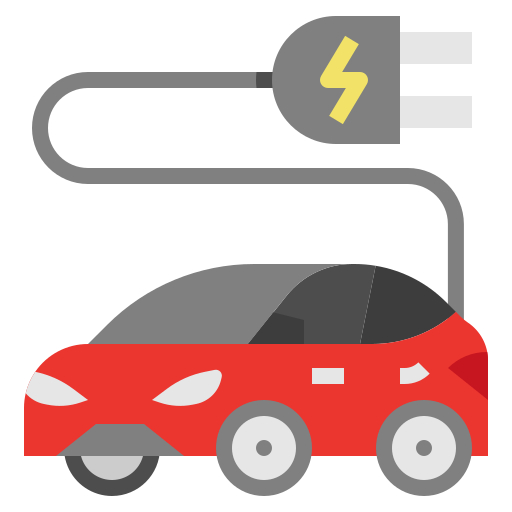
\includegraphics[width=1cm]{figures/electric-car.png}
	\hspace{2cm}
	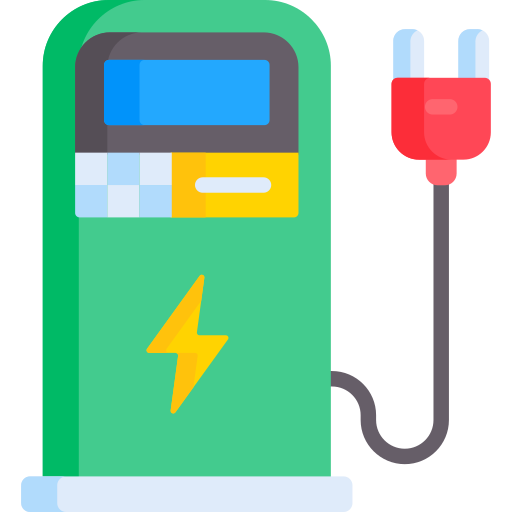
\includegraphics[width=1cm]{figures/charging.png}
    \end{figure}
\par Example of London and Reunion Island cases
\par Two (2) simulation models
\note{
Cette thèse s'inscrit dans le cadre d'un sous-thème développé par notre groupe de travail système collectif adaptatif (SCA) sur lequel nous travaillons avec des chercheurs de l'Imperial College London et la mairie de Saint-Denis de La Réunion. Dans ce cadre nous avons développé deux modèles de simulations multi-agents que nous avons particulièrement appliqué sur Londres et sur La Réunion. Nous travaillons sur 2 modèles de simulations multi-agents.
}
    
\end{frame}

\begin{frame}{Context}{SmartCityModel\footnote{
    RALITERA, Tahina, FERARD, Maxime, BUSTOS-TURU, Gonzalo, et al. Steps Towards Simulating Smart Cities and Smart Islands with a Shared Generic Framework. In : Proceedings of the 6th International Conference on Smart Cities and Green ICT Systems. SCITEPRESS-Science and Technology Publications, Lda, 2017. p. 329-336.
    \medbreak
    RALITERA, Tahina et COURDIER, Rémy. Toward Smart Island Simulation Application. In : International Conference on Practical Applications of Agents and Multi-Agent Systems. Springer, Cham, 2017. p. 457-469.}}
\begin{figure}
    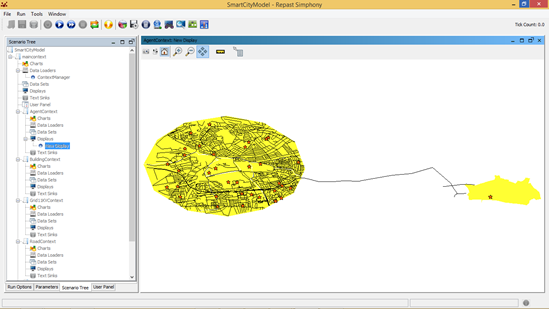
\includegraphics[width=.6\linewidth]{figures/smartCityModel.png}
    \caption{\textbf{SmartCityModel} built upon the \textbf{Repast Simphony} multi-agent simulation platform and using SIG} 
\end{figure}
\note{


\par Le premier est SmartCityModel : qui a été utilisé pour différents scénario mais qui dans notre cadre a été utilisé pour la simulation de flux de mobilité de véhicules électriques sur un territoire. Il s'agit d'un modèle développé à l'origine par les chercheurs de l'ICL sur lequel nous avons contribué. Cela a notamment fait l'objet de deux publications. Ce modèle de simulation tourne sur la plateforme développée à l'internationale Repast Simphony. Vous pouvez notamment voir ici une capture d'écran de l'interface utilisateur de la simulation. Les agents sont des conducteurs de véhicules électriques ou/et des bornes de recharges électriques. Les voitures électriques sont affichées sous forme d'étoiles orange, ils se déplacent le long des routes qui sont affichées sous forme de lignes noirs.
Cet environnement spatial est modélisé à partir de données SIG, coordonnées réelles.
}
\end{frame}

\begin{frame}{Context}{Simulation Models \footnote{AKY, Nathan, TAHINA, Ralitera, PAYET, Denis, et al. SkuadCityModel: Une simulation de déplacements urbains construite sur la plate-forme SKUAD. In : Journées Francophones Systèmes Multi-Agents (JFSMA'16)-Demonstration. Cepadues, 2018. p. 233-234.}}

\begin{figure}
    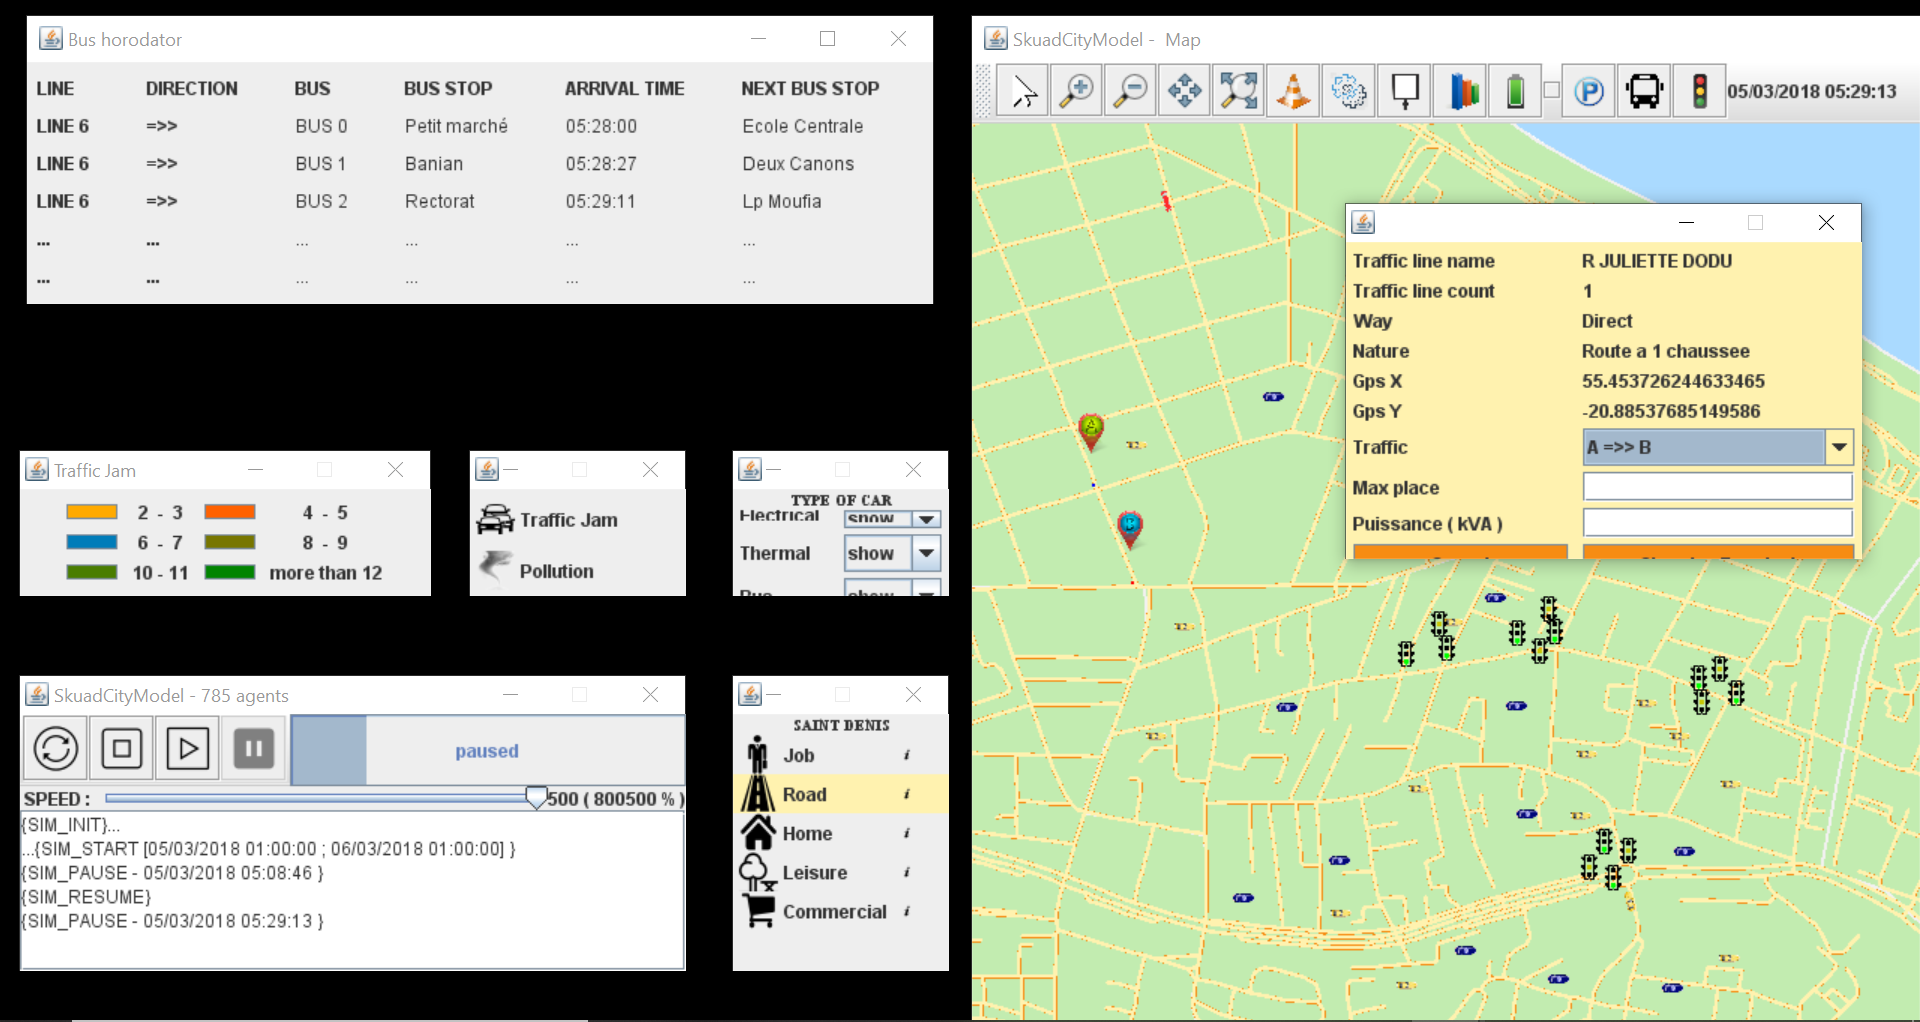
\includegraphics[width=.6\linewidth]{figures/skuadCityModelGUI.png}
    \caption{\textbf{SkuadCityModel} built upon the \textbf{SimSKUAD} multi-agent simulation platform and using SIG}
\end{figure}

\note{
\par  SkuadCityModel : est un modèle développée par notre équipe de travail. Il est inspirée de SmartCityModel et tourne sur SimSKUAD, une plateforme de simulation développée au sein de notre équipe. Voici une capture d'écran de l'interface utilisateur de la simulation. Vous pouvez notamment voir les voitures thermiques en bleu, électriques en jaune, les bornes de recharges électriques, les bâtiment, les routes ainsi que les feu de signalisation.
\par Tout cet environnement spatial que vous pouvez voir sur les captures d'écran est modélisé sur la base de données réelles sous format SIG.

}
\end{frame}

\begin{frame}{Context}{A wealth of untapped information on temporal behaviours}
\begin{figure}
    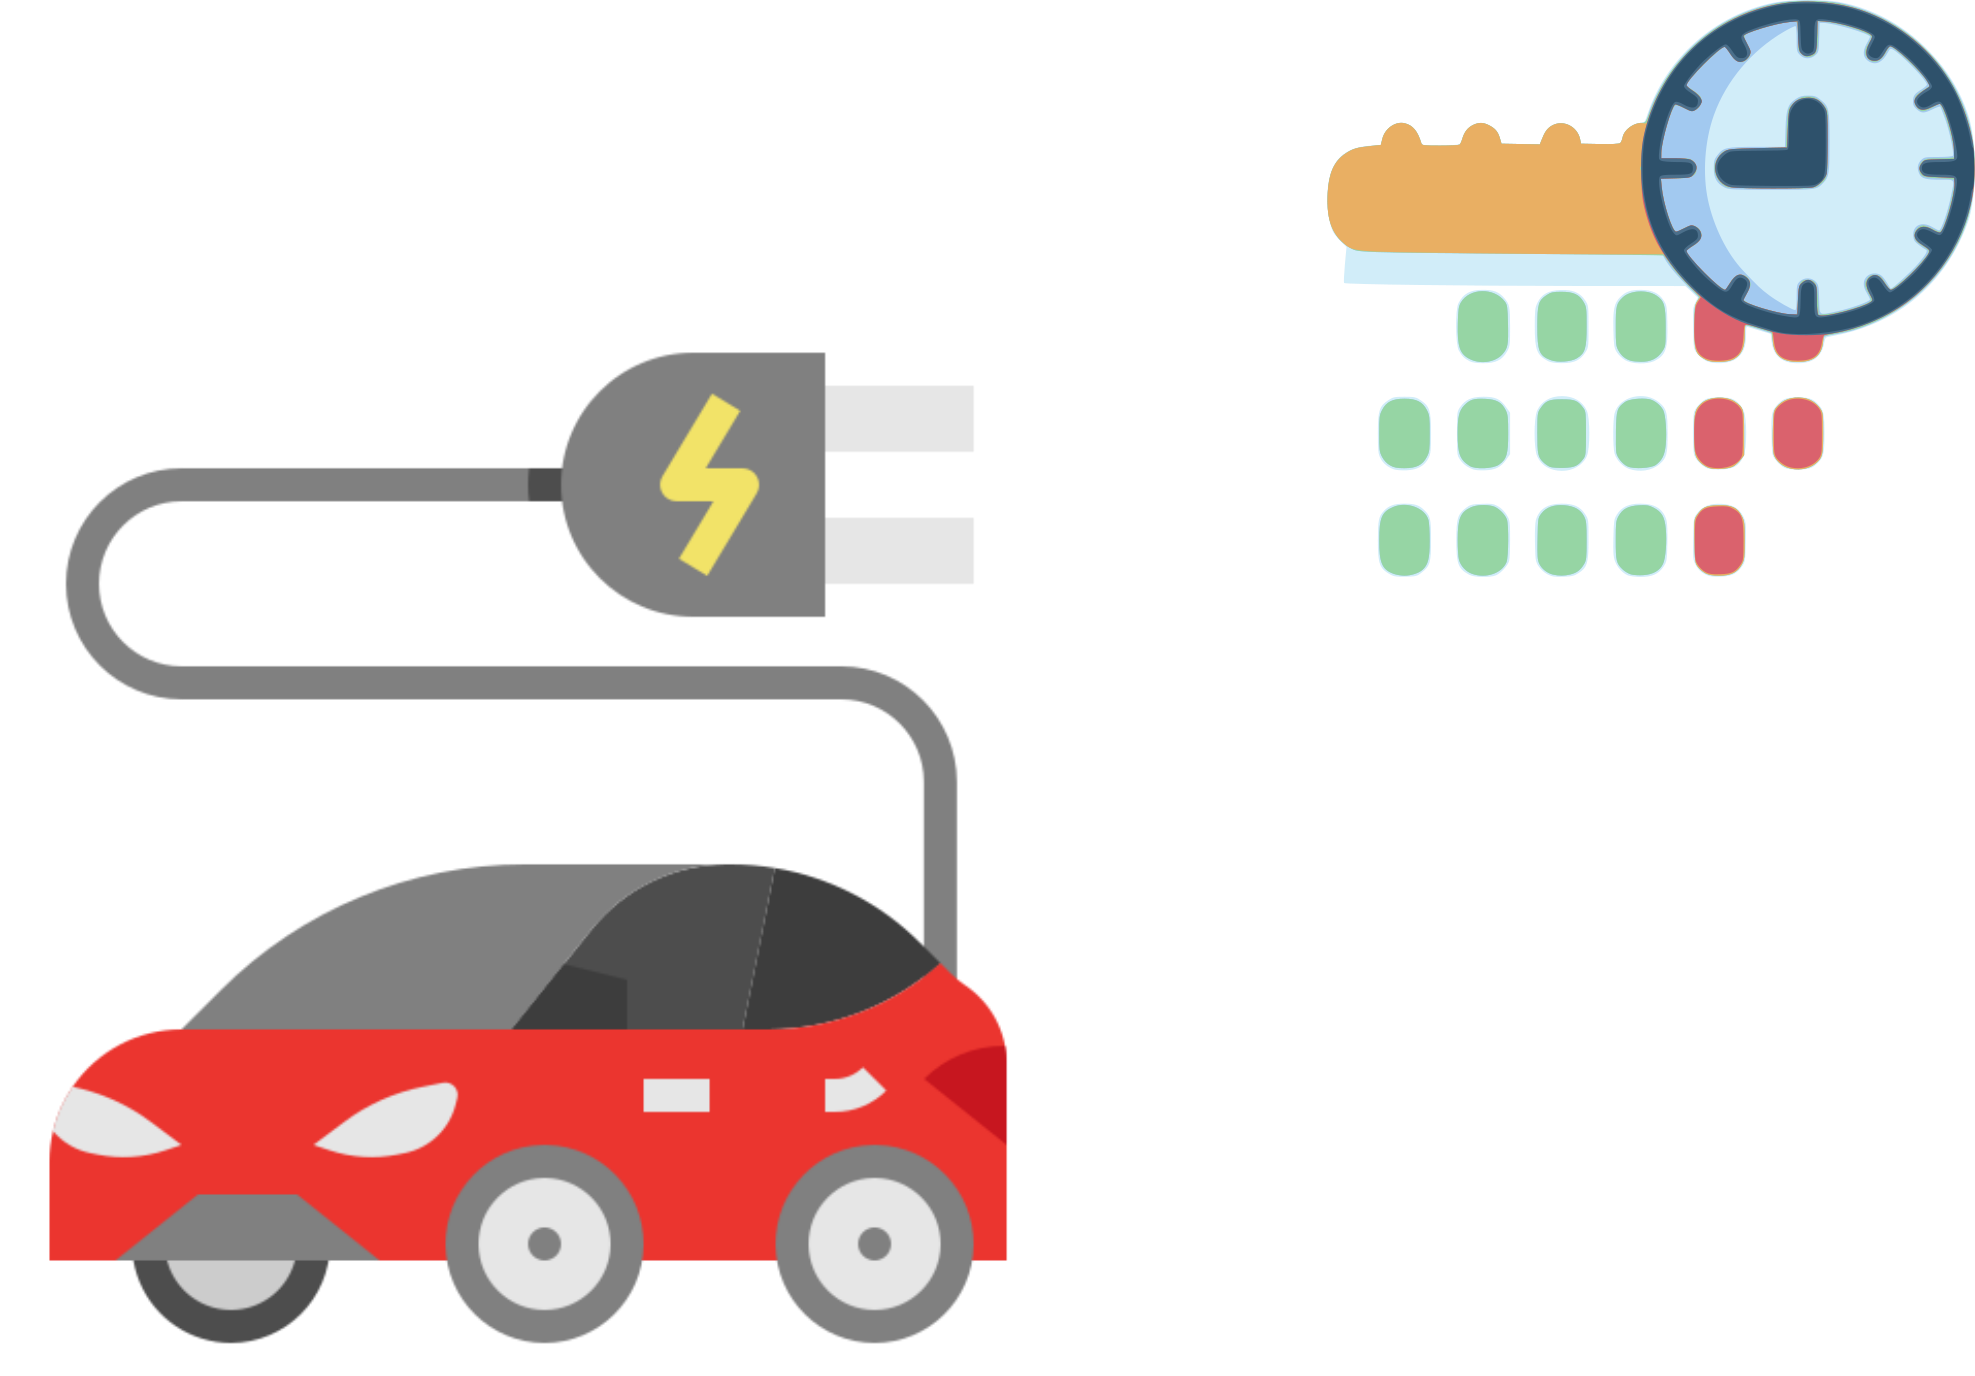
\includegraphics[width=.5\linewidth]{figures/planning.png}
\end{figure}
\par \alert{Activity-based model}
        \begin{itemize}
            \item the movements result from the activities that the agents wish or have to perform
            \item the agents own an activity planning
        \end{itemize}
\note{
\par Par ailleurs, ces modèles sont des modèles basées sur les activités, c'est-à-dire que les déplacements des véhicules électriques résultent des activités que les agents souhaitent ou doivent effectuer. Les agents disposent alors d'un planning d'activités plus ou moins défini à l'avance. Ce planning est également défini à partir de données statistiques réelles.
\par Nous pouvons donc constater une richesse d'information que nos agents peuvent exploiter au niveau de leur raisonnements. 

}
\end{frame}

\begin{frame}{Context}{A wealth of untapped information on temporal behaviours}
    \begin{figure}
    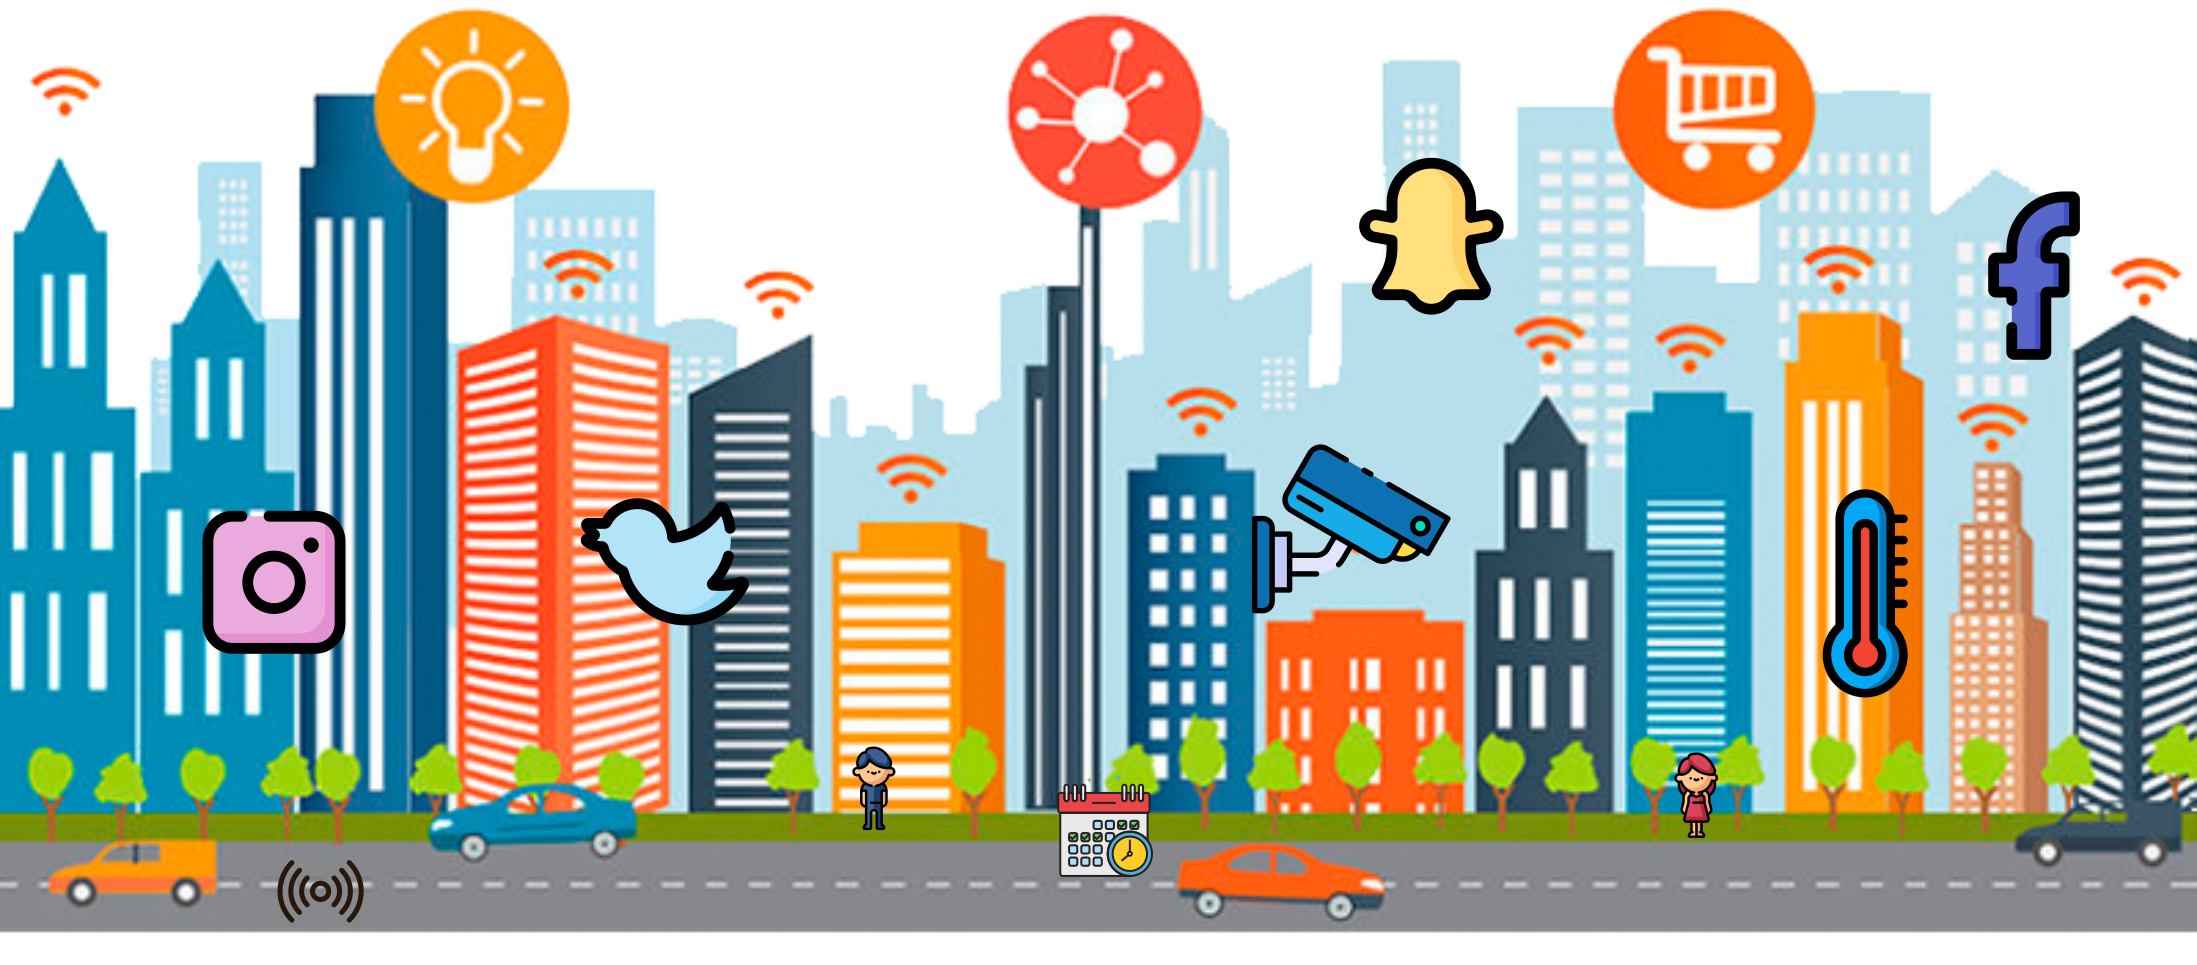
\includegraphics[width=.7\linewidth]{figures/smartcity.png}
\end{figure}
\par A wealth of spatial, social and temporal information in smart cities and smart city simulations
    \begin{itemize}
        \item \textit{How to reduce the number of possible cases?
        \item How to ensure that the agents carry out the actions that are really necessary?}
    \end{itemize}
\alert{$\rightarrow$ An anticipatory reasoning}

\note{
\par Cette richesse d'information se retrouve de manière générale au niveau de la ville intelligente et dons au niveau des simulations multi-agents pour les villes intelligente comme celles sur lesquelles nous travaillons. En effet, une ville intelligente est généralement instrumentée et dispose d'un ensemble de capteurs et d'un ensembles d'outils permettant l'échange d'une grande quantité d'informations spatiales, sociales et temporelles. 
\par Face à cette quantité d'informations phénoménale, nous pensons donc qu'il est indispensable de réduire l'ensemble des cas possibles en dotant les agents d'une capacité d'anticipation. Cela devrait leur permettre d’optimiser leur comportement en n’effectuant ainsi que les actions véritablement nécessaires. 
}
\end{frame}

\begin{frame}{Problem}{Example}

\begin{figure}
    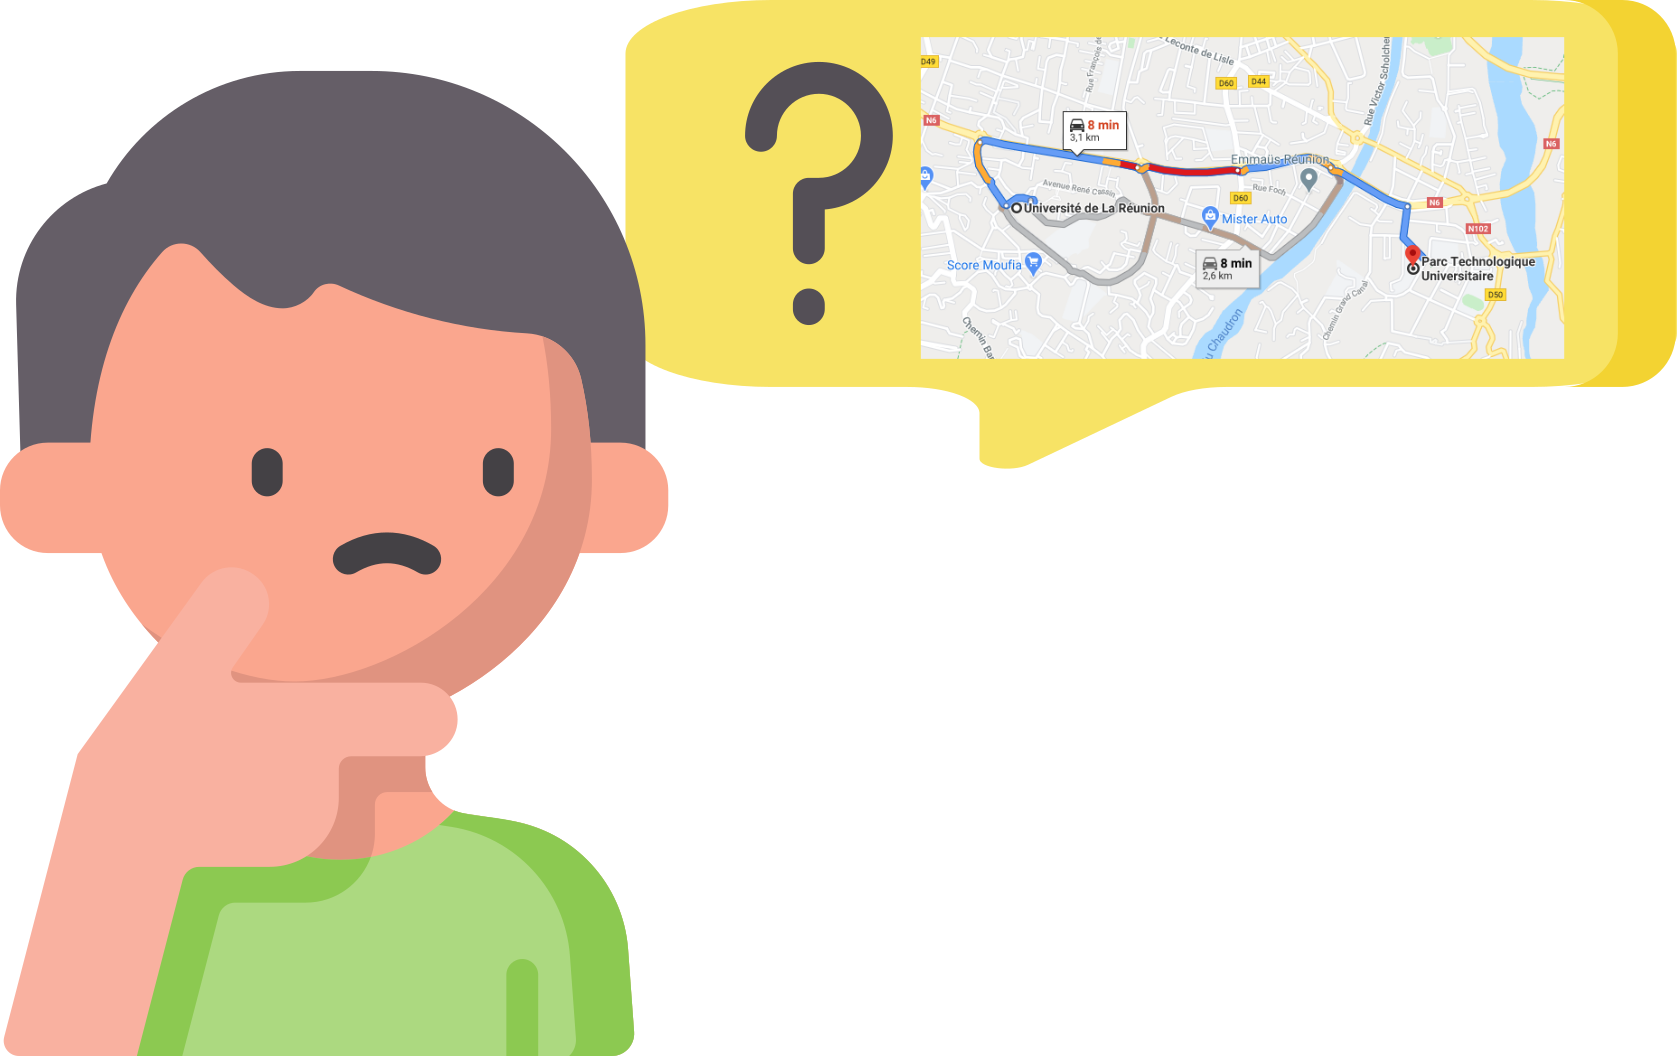
\includegraphics[width=.4\linewidth]{figures/question.png}
    \caption{ Example of the agent's anticipatory reasoning in SmartCityModel and SkuadCityModel}
\end{figure}
\par The path choice is based on the consideration of spatial dimension only: \alert{no consideration of the temporal dimension} (planning)
\note{
 Si nous prenons l'exemple du raisonnement anticipatif de l'agent dans SmartCityModel ou dans SkuadCityModel, afin de choisir un chemin parmis une liste de chemin ce dernier utilise une minimisation de la quantité prévisionnelle d'énergie requise pour effectuer le trajet. Pour cela, il prend en compte la valeur de la distance et de la pente. Aucune information temporelles, sur les projets individuelles relatives au planning d'activité des agents n'est pris en compte. Pourtant ce informations existent bel et bien au niveau de la simulation.
}
\end{frame}


\begin{frame}{Problem}{A wealth of untapped information on temporal behaviours}
\begin{enumerate}
    \item A weak consideration of temporal information compared to spatial and social information in multi-agent anticipation reasoning
    \begin{itemize}
        \item \textit{How to use temporal information in the same way as spatial and organisational information?}
    \end{itemize}
\vspace{.5cm}
    \item No consideration of information about the future (project) at the level of anticipatory reasoning
\begin{itemize}
    \item \textit{How can we provide visibility on the future dimension of time?}
\end{itemize}
\vspace{.5cm}
\alert{$\rightarrow$ An environment for the representation of the agents temporal behaviour}
\end{enumerate} 



\note{
\par Ce même constat s'applique de manière plus générale, au niveau de la plupart des raisonnements anticipatifs au niveau des agents dans les SMA. Nous constatons une faible prise en compte de la dimensions temporelle face aux dimensions spatiales et sociales. De plus, si nous nous concentrons particulièrement sur la prise en compte de la dimension temporelle dans le raisonnements anticipatif des agents, dans la majorité des approches que nous pouvons rencontrer dans la littérature, les agents prennent uniquement en compte, dans leur modèle prédictif, les informations sur le passé et sur le présent pour prédire les informations sur le futur. Aucune information sur les projets, sur le planning d'activité (futur) des agents n'est prise en compte. Cela est du au fait qu'il n'existe au sein du système aucune représentation de la dimension temps qui permette aux agents d'avoir une visibilité sur cette dimension futur du temps.
\par Nous pensons alors qu'il est insispensable de mettre en oeuvre, au niveau de la simulation, un support de représentation du comportement temporel relatif au planning d'activité des agents. Ce support devrait permettre l'échange d'information temporel et son exploitation au même titre que les informations spatiales et sociales.
}
\end{frame}

\begin{frame}{Contributions}
\begin{enumerate}
\Huge{
   \centering{ \item A temporal environment}\\}
   \medbreak
     \par \centering{ \normalsize{Temporal representation}\\}
    \par \Huge{\centering{$\Downarrow$}}
    \Huge{
    \centering{\item A consideration of the future information in anticipatory reasonning}\\}
    \centering{\normalsize{Temporal reasoning}}
\end{enumerate}

\note{
\par Face à ces besoins, nous proposons d'améliorer les simulations multi-agents sur deux niveaux:
\begin{itemize}
    \item Au niveau de la représentation du temps : nous proposons de faire évoluer les simulations multi-agents de manière à considérer le temps comme un milieu d'intéraction, au même titre que l'espace et l'organisation. Cela devrait permettre une visibilité sur le comportement temporel des agent, plus particulièrement sur la dynamique d'activation temporelle future des agents.
    \item Au niveau du raisonnement temporel, nous proposons d'enrichir le raisonnement anticipatif des agents par une prise en compte des informations sur la dimension futur du temps permise par la visibilité sur la dimension futur offerte par le support de représentation qui constitue notre première contribution.
\end{itemize}
}
    
\end{frame}

% La table des matières
\begin{frame}[plain]
 \frametitle{Outline}
 \tableofcontents
\end{frame}

%\section{Time, space and organizations MAS}
%\begin{frame}{The Multi-agent simulation}
\begin{block}{Simulation model}
\begin{columns}
\begin{column}{.18\linewidth}
    \begin{figure}
	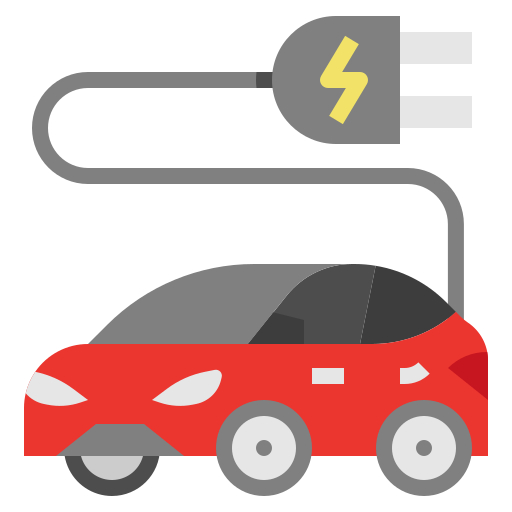
\includegraphics[width=.4\textwidth]{figures/electric-car.png}
	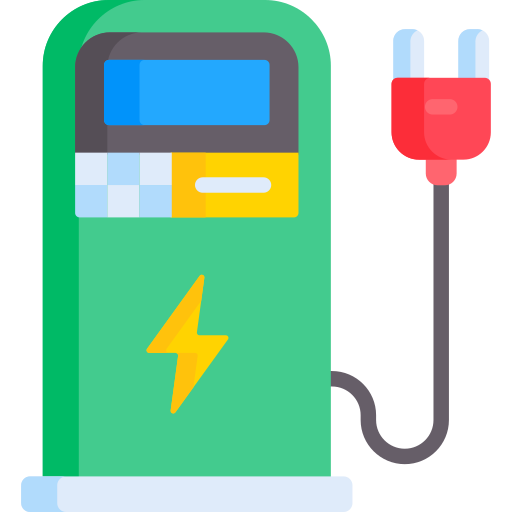
\includegraphics[width=.4\textwidth]{figures/charging.png}
    \end{figure}
\end{column}
\begin{column}{.78\linewidth}
\begin{itemize}
    \item Ex: SkuadCityModel, SmartCityModel
    \item Schematic representation of reality in order to study and to understand it
    \item Composed of a set of autonomous entities (agents) located in environments and interacting according to relationships
    \item \alert{Space} and \alert{organization} are modeled as \alert{environments} : allows the exchange of spatial and social information
    \item Agent behavioural cycle: perception, decision, action/influence 
\end{itemize}
\end{column}
\end{columns}
\end{block}
\begin{block}{Simulation platform}
\end{block}


\note{
Une simulation multi-agents peut se diviser en deux grandes parties: la plateforme de simulation et le modèle de simulation. Le modèle de simulation propose une représentation schématique de la réalité en vue de l’étudier et de la comprendre. Il est composé des agents, des environnements ainsi que des relations qui les permettent d'interagir. Dans la plupart des modèles, l’environnement est soit un environnement spatial, soit un environnement de communication dont un cas particulier est l’environnement social. Ces environnements permettent aux agent d'échanger des données relatives aux contextes d’activation spatiales et sociales. La relation entre l’agent et son environnement se traduit par le fait que l’agent agit ou exerce une influence sur son environnement et le perçoit.  Le cycle comportemental classique d’un agent se résume alors en trois phases: une phase de perception où il récolte des informations contenues au niveau de l’environnement, une phase de délibération où l’agent active son processus de raisonnement et choisi un comportement à exécuter en fonction des percepts qu’il aura récolté et de son état interne et une phase d'action ou d’influence où l’agent agit ou essaie d’agir sur son environnement.
}
\end{frame}

\begin{frame}{The Multi-agent simulation}
\begin{block}{Simulation model}
\end{block}
\begin{block}{Simulation platform}
\begin{columns}
\begin{column}{.18\linewidth}
    \begin{figure}
	
\includegraphics[width=.4\textwidth]{figures/code.png}
	
\includegraphics[width=.4\textwidth]{figures/calendar.png}
    \end{figure}
\end{column}
\begin{column}{.78\linewidth}
\begin{itemize}
    \item Ex : SimSKUAD, Repast Simphony
    \item Dedicated to multi-agent simulation development
    \item Contain libraries that facilitates the development of multi-agent simulation. Ex: the scheduler
\end{itemize}
\end{column}
\end{columns}
\end{block}


\note{
La plateforme de simulation multi-agents est dédiée au développement de systèmes et simulations multi-agent. Elle peut contenir un ensemble de librairies facilitant le développement d'un modèle de simulation. Plus particulièrement, puisque nous nous intéressons au temps, les plateformes de simulation comme celles que nous utilisons dans le cadre de cette thèse contiennent l'ordonnanceur de la simulation. }
    
\end{frame}

\begin{frame}{The Time management in multi-agent simulation}
\begin{block}{The Scheduler}
\begin{itemize}
        \item Is responsible for the simulation activation cycle
        \item Consists of a mechanism that makes time run out, activates the agents and updates the environments according to a virtual clock (\textbf{simulated time} $\ne$ real time)
        \item Uses time scheduling approaches. Ex : time-stepped, event-driven, hybrid, temporality model
    \end{itemize}
\vspace{.5cm}
\textbf{Main limit}: No access to (no exchange of) information about the agents temporal activation dynamic
\end{block}
    
    \note{
    
    Cet ordonnanceur est responsable de la gestion du temps en terme de cycle d’activation de la simulation. Son fonctionnement consiste en une mécanique qui fait écouler le temps, qui active les agents et met à jour les environnements en fonction d’une horloge virtuelle. Nous parlons notamment de temps simulé qui est le reflet de notre temps réel, astronomique. C'est le temps qui est mesuré par une horloge virtuelle intégrée dans le simulateur. Pour gérer ce temps simulé, l’ordonnanceur utilise différentes approches d’ordonnancement : à pas de temps constant, événementielle, hybride, etc. La manière dont le temps est géré est différent selon l’approche utilisé, ainsi chaque approche peut avoir ses avantages et ses limites. Cependant celle que nous retiendrons est le fait qu'aucune approche ne permet aux agents, l'accès aux informations sur leurs dynamique d'activation temporelle.
    
    }
\end{frame}

\begin{frame}{The Time management in multi-agent simulation}
%flèche dans les deux sens ambigüe
\begin{columns}
\begin{column}{.18\linewidth}
    \begin{figure}
	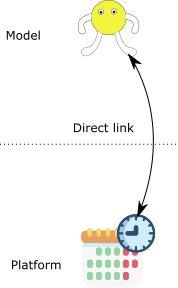
\includegraphics[width=1.2\textwidth]{figures/agentsVSscheduler.png}
    \end{figure}
\end{column}
\begin{column}{.78\linewidth}
\textbf{Process}:
\begin{itemize}
    \item The agent or the simulation model determines the activation rythm and communicates it to the scheduler
    \item The scheduler activates the agents based on this information.
\end{itemize}
    \vspace{1cm}
\par \textbf{Main limit}: no exchange of information about the agents temporal activation dynamics
        \begin{itemize}
            \item  Sharing temporal activation dynamics information is possible
            \item Access to temporal activation dynamics information is not possible (a key smart cities effectiveness)
            \item Taking into into account \say{non-existent} information in the agents reasoning is not possible
        \end{itemize}

\end{column}
\end{columns}
    
\note{
De manière générale, la relation entre l’agent et l’ordonnanceur se fait par lien direct. En fonction de l'approche d'ordonnancement utilisé, l'agent ou le modèle de simulation détermine le rythme d’activation et le communique à l'ordonnanceur de la simulation, au niveau de la plateforme de simulation. L’ordonnanceur active donc les agents en fonction de ces informations. Le traitement de l’information se fait dans un seul sens : aucun échange d’informations ne peut être effectué au niveau de la dimension temporelle: l'agent partage des informations sur sa dynamique temporlle mais n'a pas accès à ces informations partagées donc impossible de les prendre en compte au niveau du raisonnement. Voyons plus en détails comment nos propositions permettent de nous affranchir de ces limites.


}
\end{frame}

%\section{Contributions}
\section{Time Representation}
\begin{frame}{Time, space and organization representation in multi-agent simulation}
\begin{columns}
\visible<1->{\begin{column}{.50\linewidth}
\vspace{.6cm}
\begin{figure}
    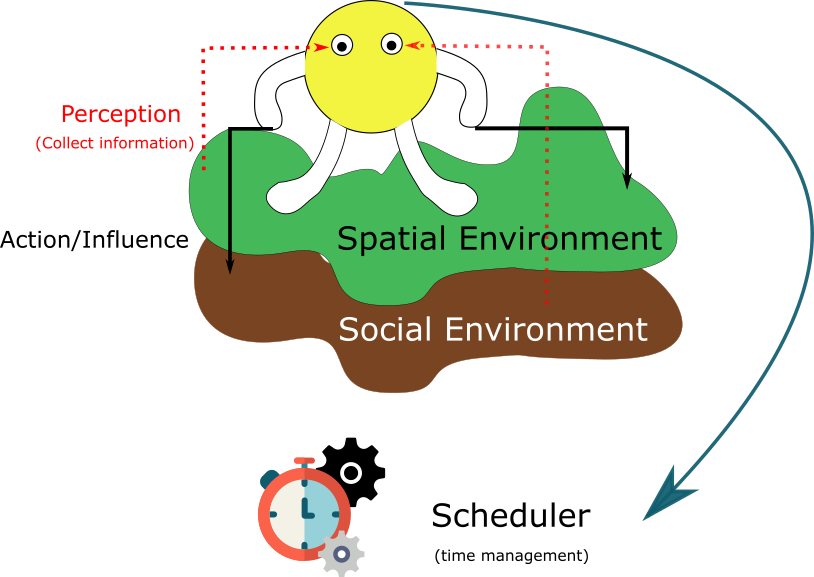
\includegraphics[width=.85\linewidth]{figures/before.png}
    \caption{MAS classical approach}
\end{figure}
\end{column}}
\visible<2->{
\begin{column}{.50\linewidth}
\begin{figure}
    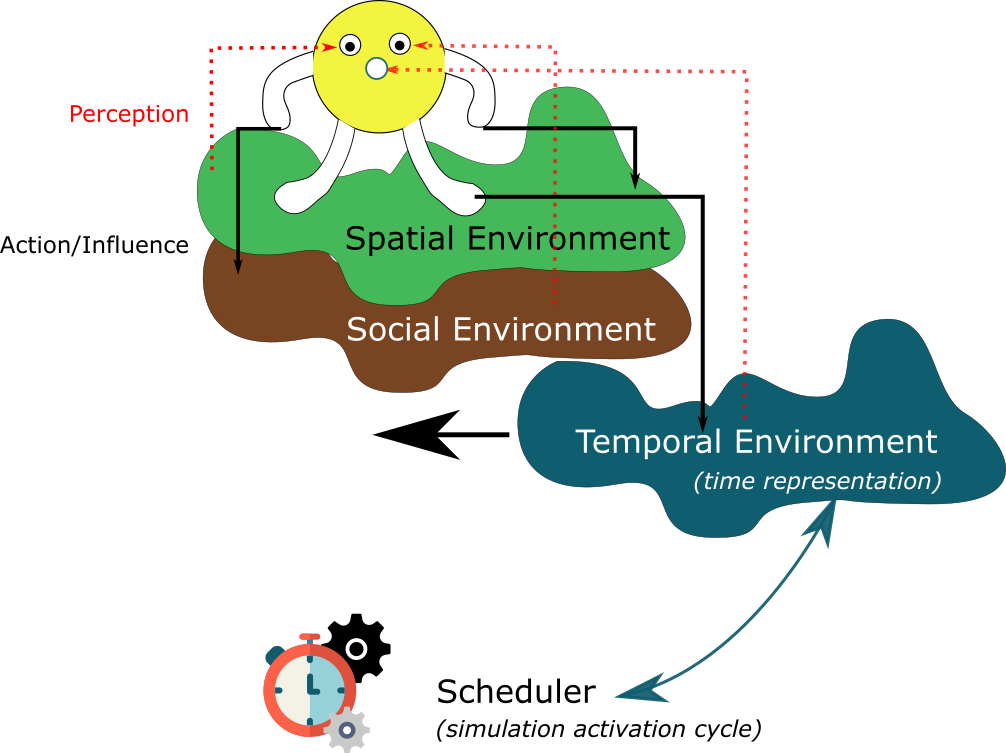
\includegraphics[width=\linewidth]{figures/after.png}
     \caption{Our proposition}
\end{figure}
\end{column}}
\end{columns}
\note{
\par Dans beaucoup d'approches dans les simulations multi-agents, l'espace comme les organisations sont modélisé sous la forme d'environnements. Ces environnements spatiales et sociales permettent aux agents de partager et d'accéder à des informations sur leur contexte d'activation spatial et social.
\par Contrairement à cela, de manière générale, le temps est abordé uniquement sous l'angle technique, en tant que mécanique de la simulation. Il est géré au niveau d'une entité de la plateforme de simulation appelé ordonnanceur. Le fonctionnement de l'ordonnanceur consiste à gérer le cycle d'activation de la simulation, en faisant s'écouler virtuellement le temps. L'ensemble des connaissances concernant le comportement temporel des agents est alors accessible et exploité uniquement par l'ordonnanceur de la simulation. 
\par Afin de permettre aux agents d'avoir une visibilité sur cette dynamique d'activation temporelle et de l'exploiter, nous proposons de compléter le fonctionnement de l'ordonnanceur de la simulation par un milieu d'interaction que nous appelons l'environnement temporel. Désormais, la gestion du temps au niveau de la simulation multi-agents se faire sur deux niveaux:
\begin{itemize}
    \item Au niveau de l'environnement temporel : qui sert de support permettant aux agents de partager et de percevoir les informations sur leur comportement temporel
    \item Au niveau de l'ordonnanceur de la simulation : qui gère l'écoulement du temps et le cycle d'activation de la simulation
\end{itemize}
}
    
\end{frame}

\begin{frame}{The Temporal Environment}{General architecture}
\par \textbf{Objective}: evolve multi-agent simulations in such a way as to consider time as a medium of interaction, in the same way as space or organisations.
\vspace{1cm}
\par \textbf{Proposition}:

\begin{columns}
\begin{column}{.3\linewidth}
\begin{figure}
    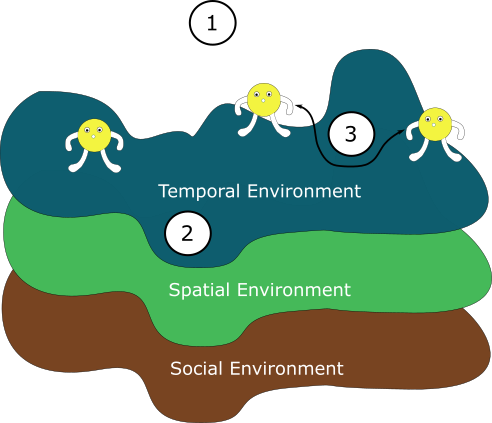
\includegraphics[width=\linewidth]{figures/temporalRepresentation.png}
\end{figure}
\end{column}
\begin{column}{.7\linewidth}
\begin{enumerate}
    \item The \textbf{Agent-Group-Role-Environment-Time (AGRET)} model
    \item The \textbf{temporal environment}\footnote{RALITERA, Tahina, PAYET, Denis, et COURDIER, Rémy. Toward a Temporal Environment for Multi-Agent Simulation. Journal of Communications, 2019, vol. 14, no 7.}
    \item The Influence-Reaction Model For Simulation (IRM4S) \footnote{MICHEL, Fabien. The IRM4S model: the influence/reaction principle for multiagent based simulation. In : Proceedings of the 6th international joint conference on Autonomous agents and multiagent systems. 2007. p. 1-3.}
\end{enumerate}
\end{column}
\end{columns}
\note{
Notre objectif est de faire évoluer les simulations multi-agents de manière à considérer le temps comme un milieu d'interaction, au même titre que l'espace ou les organisations. Ce nouveau milieu d'interaction s'appelle l'environnement temporel et peut se définir de manière très simple comme un espace dont la métrique est le temps. L'agent est capable de percevoir et d'agir sur son environnement temporel selon le modèle IRM4S, un modèle d'interaction de type influence/réaction spécialement conçu pour la simulation.
\par Pour mettre en place ce nouvel environnement au sein du système existant, nous proposons une méthodologie de conception permettant d’articuler les 3 dimensions spatiale, organisationnelle et temporelle. Nous appelons cette approche AGRET. AGRET étend l'approche AGRE en y rajoutant la prise en compte de l'environnement temporelle au même titre que les environnements spatiales et sociales. AGRE est elle même une extension du modèle générique d'organisation AGR qui rajoute la prise en compte de l'environnement spatiale à la prise en compte de la dimensions sociale qui est faite au niveau d'AGR.
}  
\end{frame}

\begin{frame}{The temporal Environment}{Structure}
\begin{columns}
\visible<1->{
\begin{column}{.33\linewidth}
\begin{figure}
    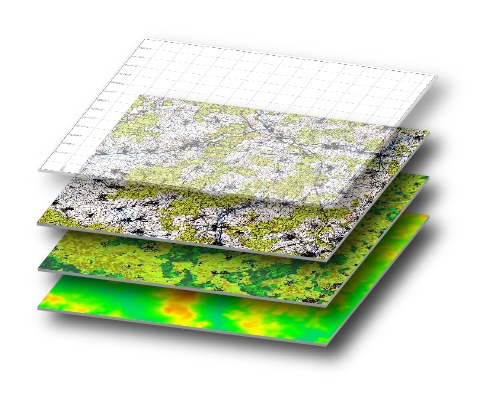
\includegraphics[width=\linewidth]{figures/space.png}
    \caption{The \textbf{spatial} environment structure.\medbreak \textit{Ex: GIS, grid, continuous space, etc.}}
\end{figure}
\end{column}
\begin{column}{.33\linewidth}
\begin{figure}
    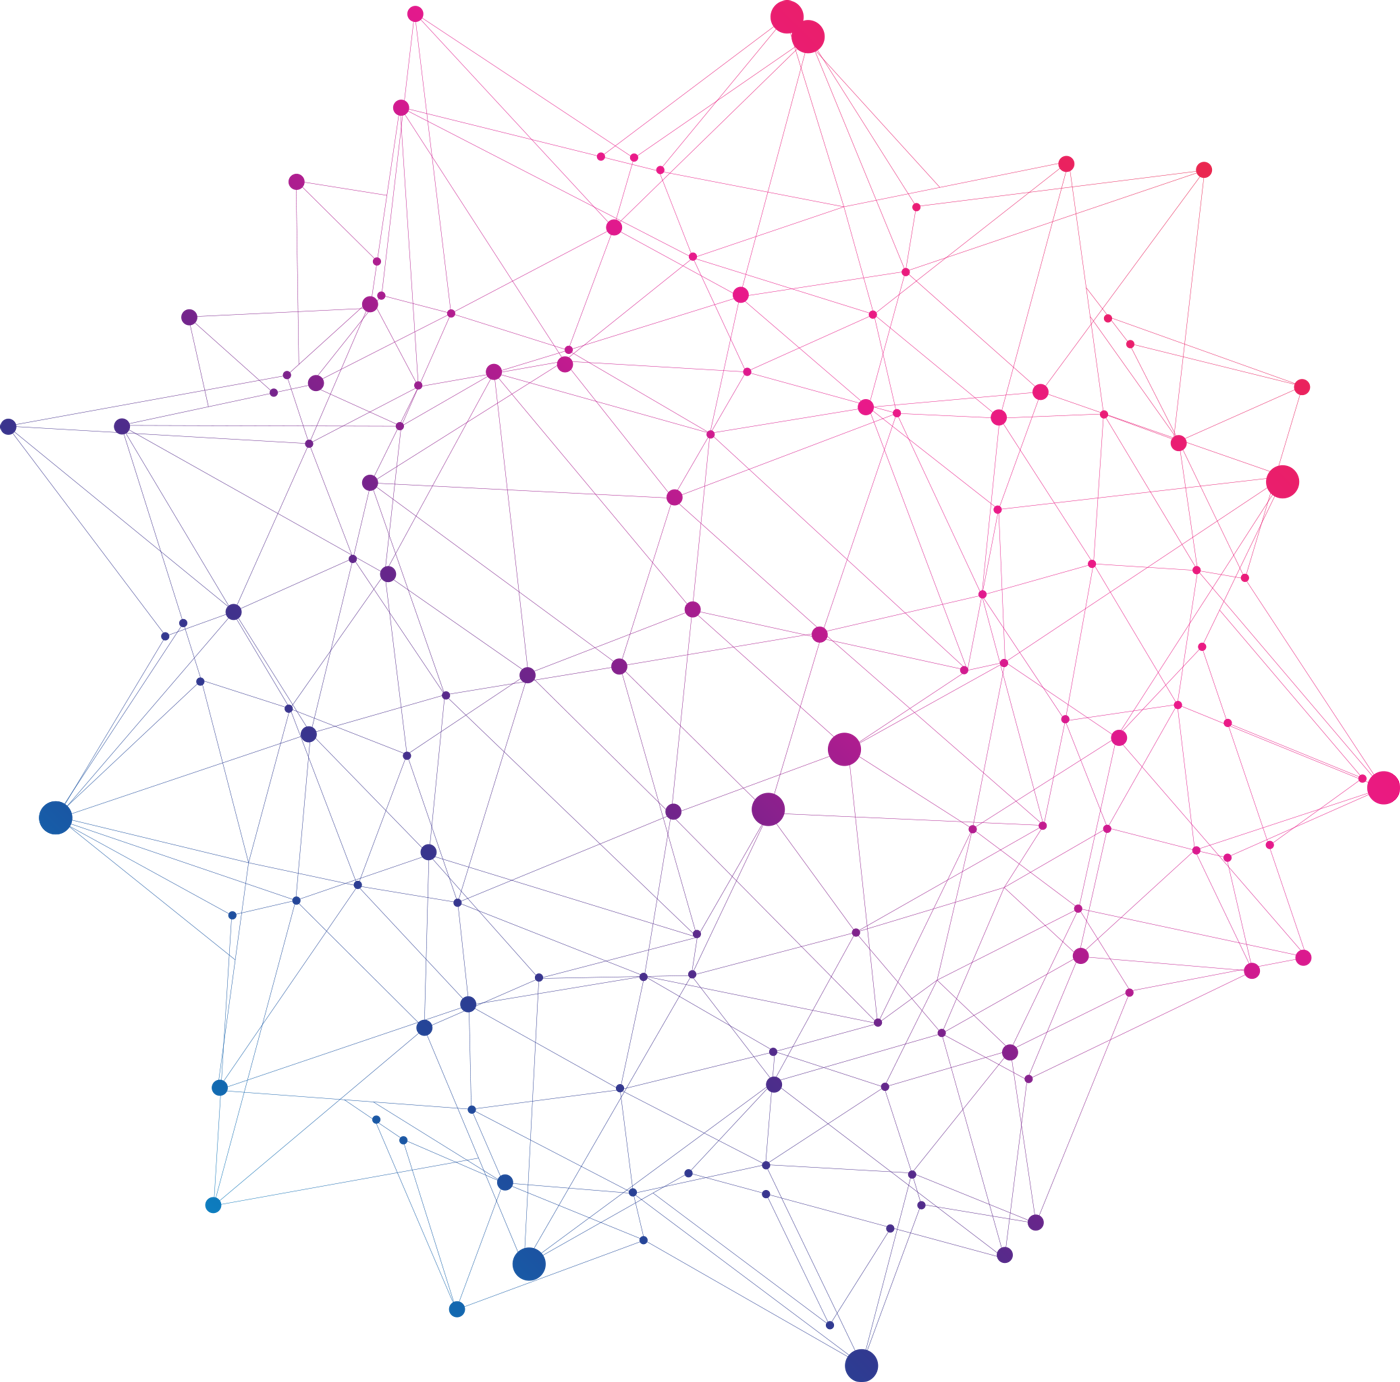
\includegraphics[width=.75\linewidth]{figures/social.png}
    \caption{The \textbf{social} environment structure.\medbreak \textit{Ex: Network}}
\end{figure}
\end{column}}
\visible<2->{\begin{column}{.33\linewidth}
\vspace{1cm}
\begin{figure}
    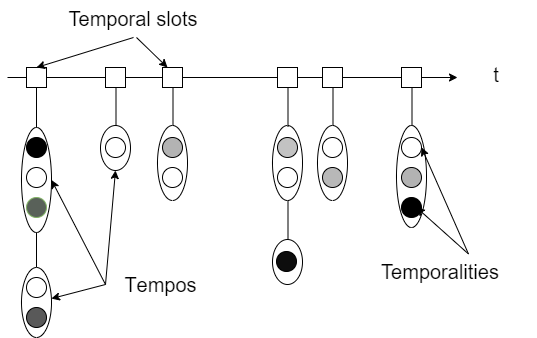
\includegraphics[width=\linewidth]{figures/temporalityModel.png}
    \caption{The \textbf{temporal} environment structure.\medbreak \textit{\alert{The temporality model}}}
\end{figure}
\vspace{.5cm}
\end{column}}
\end{columns}

\note{
Chaque environnement possède une structure et des mécaniques qui lui sont propre. Par exemple, l'environnement spatial peut être structuré à partir de données SIG, de grilles, d'espace continu, l'environnement social peut être structuré à partir de réseaux. Dans notre proposition, l'environnement temporel est structuré sur la base d'une approche appelée modèle à Temporalité.
\par Le modèle à temporalité est une approche qui à l'origine a été conçu pour l'ordonnancement de la simulation, au même titre que l'approche à pas de temps constant ou l'approche événementielle. Il permet aux agents d'exprimer leur dynamique d'activation temporelle et de les partager à l'ordonnanceur de la simulation. Au niveau de l'ordonnanceur, cette dynamique est représentée sous la forme de temporalité, agrégé à travers des tempos. Ces tempos sont rattachées à des slots temporels qui ponctuent l'axe temporel de la simulation. Une explication détaillée peut peut être lues dans nos contributions
}
    
\end{frame}

\begin{frame}{The Temporal Environment}{The Temporality Model}
\begin{figure}
    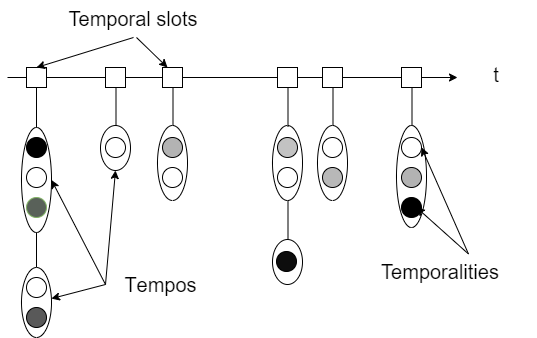
\includegraphics[width=.4\linewidth]{figures/temporalityModel.png}
    \caption{The temporality model\footnote{
PAYET, Denis, COURDIER, Rémy, RALAMBONDRAINY, Tiana, et al. Le modèle à Temporalité: pour un équilibre entre adéquation et optimisation du temps dans les simulations agent. In : JFSMA. 2006. p. 63-76.
\medbreak
RALITERA, Tahina, PAYET, Denis, AKY, Nathan, et al. The Temporality Model Time Scheduling Approach: A Practical Application. In : International Workshop on Multi-Agent Systems and Agent-Based Simulation. Springer, Cham, 2018. p. 115-125.} time axis.}
\end{figure}
\par \textbf{Model evolution} for the use in the context of the temporal environment: \alert{storage and perception} of information about the past and the future
\note{
\par Nous reprenons alors ces bases afin de structurer l'environnement temporel. Cependant, nous procédons à une extension du modèle de manière à permettre le stockage et la perception des informations sur le passé et sur le futur qui n'existait pas dans l'approche original du modèle à temporalité car cela n'était pas nécessaire compte tenu de l'objectif pour lequel il a été conçu. 
\par En effet, comme il s'agit d'une approche d'ordonnancement, l'axe temporel est située au niveau de l'ordonnanceur qui est le seul à l'exploiter. Par conséquent, seul les informations nécessaires à l'activation des agents y sont représentés et stockés. C'est à dire que les informations passées sont automatiquement effacés car elles ne servent plus à l'activation de la simulation et les informations futures sont calculées à chaque avancement du temps. Ce fonctionnement permet l'optimisation du mécanisme d'ordonnancement de la simulation.
\par Cependant, le stockage et la perception des comportements temporels passés et futurs sont indispensable dans l'usage que nous en faisons. Nous effectuons alors une refonte du modèle afin d'y intégrer ces fonctionnalités.
}
    
\end{frame}

\begin{frame}{The Temporal Environment}{Temporal information storage and perception}
\begin{figure}
    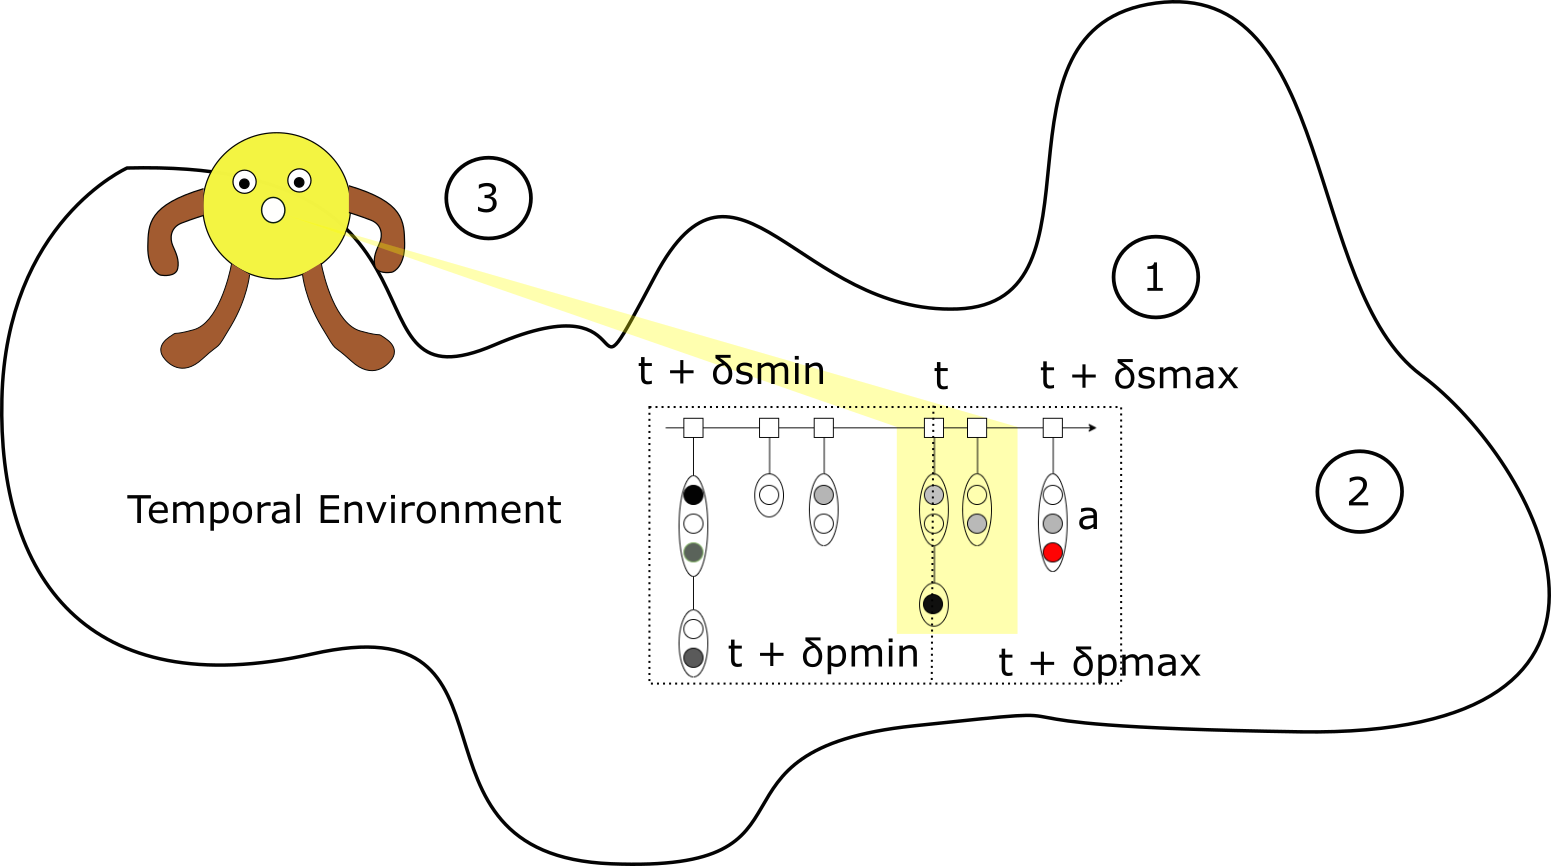
\includegraphics[width=.7\linewidth]{figures/horizon.png}
    \caption{The temporal environment: Storage and perception}
\end{figure}
\begin{enumerate}
     \item Absolute time horizon or storage time horizon of the temporal environment
     \item Accessibility rules. \textit{Ex: public or private}
    \item Relative time horizon or time horizon of perception of the agents
\end{enumerate}

\note{
Afin de gérer le stockage et la perception des informations temporelles, nous mettons en oeuvre deux contraintes:
\begin{itemize}
    \item L'horizon temporel absolu ou horizon temporel de stockage de l'environnement : elle définie une portée de stockage des informations temporelles qui est commune à tous les agents de la simulation. En effet, la pertinence de ces informations varie en fonction du temps, du modèle et du type d'information. Une information passée peut avoir une durée de vie au-delà de laquelle elle devient obsolète. De même, au-delà d'une certaine limite dans le temps, une information future n'est pas forcément pertinente. L'horizon temporel absolue permet d'optimiser le stockage en ne gardant uniquement que les informations pertinentes. La valeur de ses bornes sont définies arbitrairement par l'utilisateur ou le concepteur du modèle. Dans le modèle à temporalité, au niveau de l'ordonnanceur, la valeur de l'horizon temporel absolue est nulle. Ce qui équivaut au faut que l'axe temporel ne stocke que les informations présentes. Contrairement à cela, dans l'environnement temporel, la valeur de l'horizon temporel absolu est non nulle.
    \item L'horizon temporel relative ou horizon temporel de perception des agents : elle est propre aux caractéristiques de chaque agent et contraint sa perception. Son équivalent spatiale est le champ de vision.
\end{itemize}
}
    
\end{frame}


\begin{frame}{The Temporal Environment}{Example and implementation}
\begin{figure}
    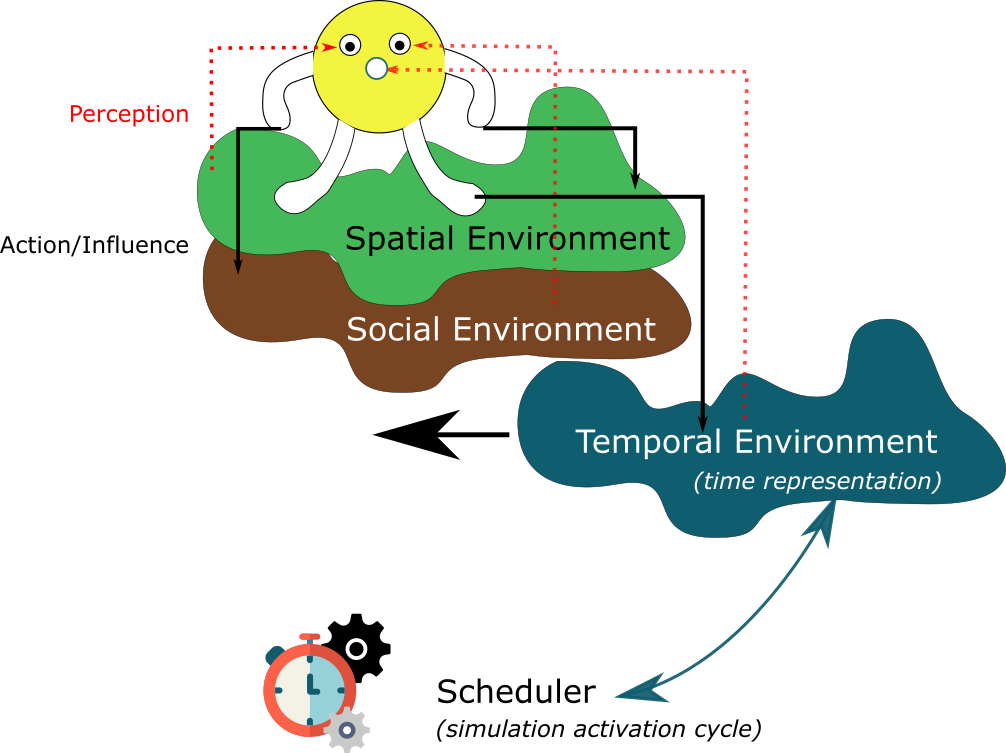
\includegraphics[width=.6\linewidth]{figures/after.png}
    \caption{Implementation of the temporal environment}
\end{figure}
\note{

\par Un autre changement, que j'ai déjà mentionné précédemment se situe au niveau du lien direct qui existait auparavant entre les agent et l'ordonnanceur de la simulation. Chaque agent communiquait directement son planning d'activité à l'ordonnanceur de la simulation qui utilisait ces informations pour activer chaque agent au moment souhaité. L'environnement temporel vient s'interfacer entre l'agent et l'ordonnanceur cassant le lien direct qui existait avant entre eux. Avant l'agent exprimait sa dynamique d'activation temporelle. Celle-ci était directement traitée au niveau de l'ordonnanceur de la simulation. Ce dernier était donc le seul à avoir accès à ces informations et l'utilisait uniquement pour la gestion de l'activation des agents et plus généralement pour la gestion du cycle d'activation de la simulation. Désormais, l'agent exprime sa dynamique d'activation temporelle, cette dernière est stockée au niveau de l'environnement temporel qui permet son accès non seulement par l'ordonnanceur de la simulation comme ce qui était déjà le cas avant mais également par les agents en fonction des horizons temporelles (absolue et relative) et d'autres règles d'accessibilité qui peuvent être définies par le modélisateur.
\par Désormais, les agents partagent leur planning au niveau de l'environnement temporel. Ce planning devient alors accessible non seulement par l'ordonnanceur mais également par les autres agents du système. Maintenant que les agents ont accès à cette information partagée sur le comportement temporel des autres agents, ils peuvent l'exploiter dans le cadre de son raisonnement. Ce qui constitue notre deuxième contribution qui consiste en l'exploitation de ces informations afin d'enrichir ceux utilisées au niveau du raisonnement anticipatif de l'agent.}

\end{frame}


\begin{frame}{The Temporal Environment}{Example and implementation}
\begin{columns}
\visible<1->{
\begin{column}{.4\linewidth}
\vspace{.3cm}
\begin{figure}
    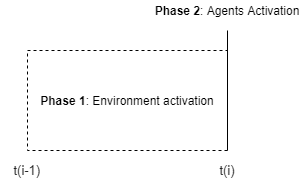
\includegraphics[width=\linewidth]{figures/old_cycle.png}
    \caption{Classical simulation activation cycle}
\end{figure}
\end{column}}
\visible<2->{
\begin{column}{.6\linewidth}
\begin{figure}
    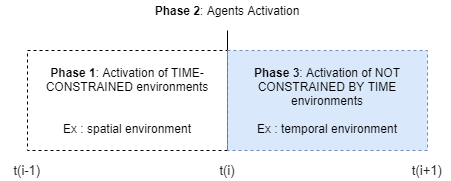
\includegraphics[width=\linewidth]{figures/new_cycle.png}
    \caption{New simulation activation cycle}
\end{figure}
\end{column}}
\end{columns}
\note{
\scriptsize{
\par La mise en place de l'environnement temporel au sein du système existant apporte de nouveaux changement. Un changement qui nous semble intéressant concerne le cycle d'activation de la simulation utilisant une approche d'interaction de type influence/réaction. Si le cycle d'activation classique consiste en 2 phases : 
\begin{itemize}
   \item Une phase d’activation de l’environnement durant laquelle le simulateur doit mettre à jour l’horloge virtuelle, initialiser le prochain cycle, etc.;
    \item Une phase d'activation des agents durant laquelle l'agent applique le processus itératif : perception, mémorisation, décision. 
\end{itemize}
L'introduction de l'environnement temporel vient chambouler ce cycle d'activation classique en scindant l'activation des environnements en deux:
\begin{itemize}
    \item L'activation des environnements contraints par le temps
    \item L'activation des environnements non contraints par le temps.
\end{itemize}
Dans la plupart des simulateurs, la phase d'activation de l'environnement se déroule en début du cycle d'activité de la simulation. Cela est dû au fait que la plupart des environnements a besoin de calculer son nouvel état en début d'un cycle (instant $t$), avant l'activation des agents. Ces calculs doivent  s'établir sur l'intervalle de temps qui s'est écoulé depuis la dernière activation. Ces environnements ont des états qui évoluent dans le temps en fonction des lois inertielles qui leur sont propres, et des influences qu'exercent les agents. Ce sont donc, en quelque sorte, des environnements contraints par le temps. Des exemple sont les environnements spatiales.
\par Dans notre contexte, par définition, l'état de l'environnement temporel détermine la dynamique d'écoulement du temps. Par conséquent, son état évolue hors du temps. \textbf{L'environnement temporel n'est donc pas un environnement contraint par le temps}. 
\par Ainsi, les 3 nouvelles phases du cycle d'activation de la simulation utilisant une approche de type influence/réaction:
\begin{enumerate}
    \item la phase d'activation des environnements contraints par le temps sur l'intervalle de temps $] ]t(i-1), t(i)]$; 
    \item la phase d'activation des agents sur le slot temporel courant $t$;
    \item la phase d'activation des environnements non contraints par le temps sur la considération que $t$ vient d'être passé.
\end{enumerate}
}
}
\end{frame}



\section{Temporal reasoning}
\begin{frame}{Anticipatory Reasoning in multi-agent simulations}
\begin{columns}
\visible<1->{
\begin{column}{.5\linewidth}
\vspace{.3cm}
\begin{figure}
    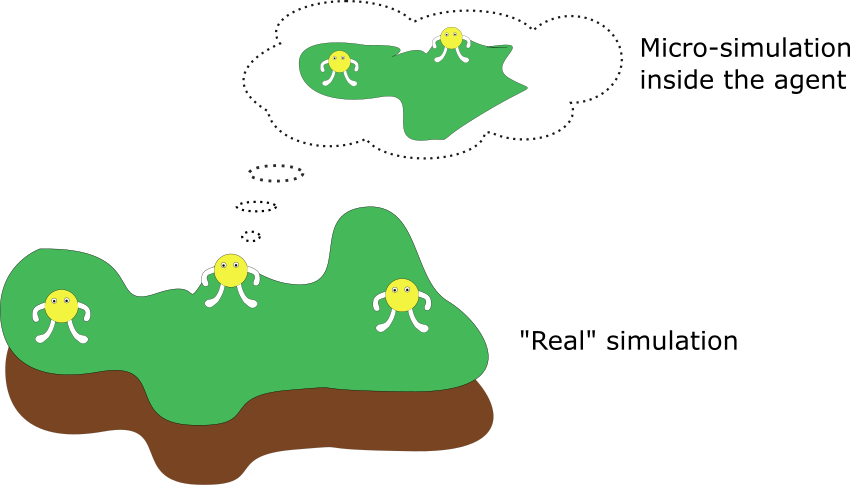
\includegraphics[width=\linewidth]{figures/classic_anticipation.png}
    \caption{Classical anticipatory reasoning}
\end{figure}

\end{column}
}
\visible<2->{
\begin{column}{.5\linewidth}
\begin{figure}
    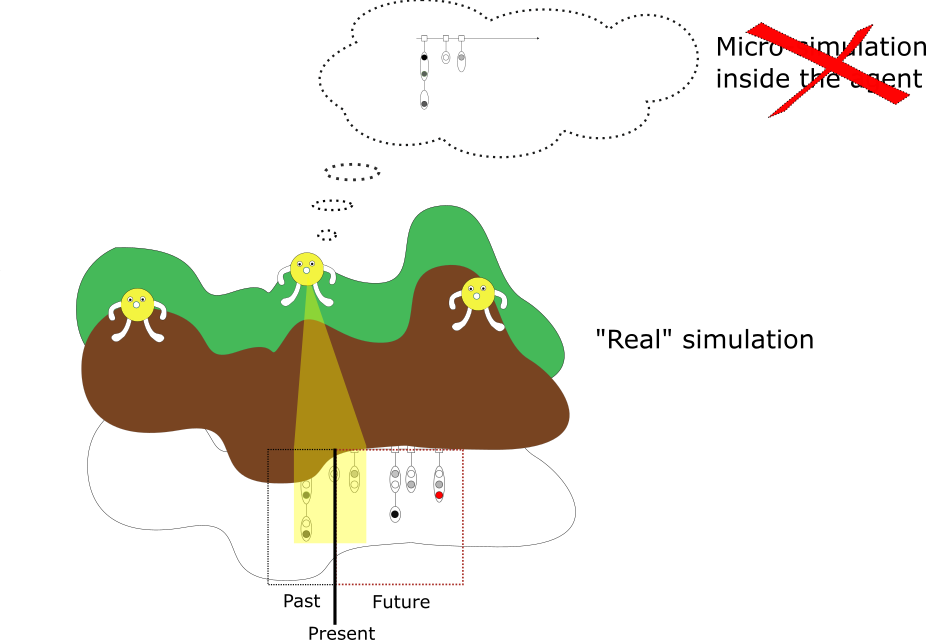
\includegraphics[width=\linewidth]{figures/new_anticipation.png}
    \caption{Anticipatory reasoning using the temporal environment perception}
\end{figure}
\end{column}
}
\end{columns}
\note{
\par Dans la plupart des approches classiques d'anticipation dans les sma, le raisonnement anticipatif prend en compte uniquement les informations sur la dimension passée et la dimension présente du temps. Dans ces types d'approches, l'agent est contraint de deviner ce qui va se passer dans le futur, car ils n'a aucune information sur le planning d'activités des autres agents. Pour se faire, les agents lancent en interne des microsimulations qui génèrent des prédictions. Dans beaucoup d'approches, ces microsimulations reproduisent tout une une partie du modèle de simulation véritablement utilisé.
\par Nous proposons donc une amélioration de ce raisonnement anticipatif par l'intégration de l'environnement temporel qui offre une nouvelle dimension d'expression et de partage entre les agents. La nature temporelle de cette nouvelle dimension permet de capter les projets individuels de chaque agent et de les diffuser sur le collectif. L'analyse prédictive réalisée par les agents peut alors opérer par perception dans ce nouvel environnement commun, plutôt que par des calculs de simulation reproduits par chacun d'eux.
}
\end{frame}

\begin{frame}{A consideration of the future}
\begin{figure}
    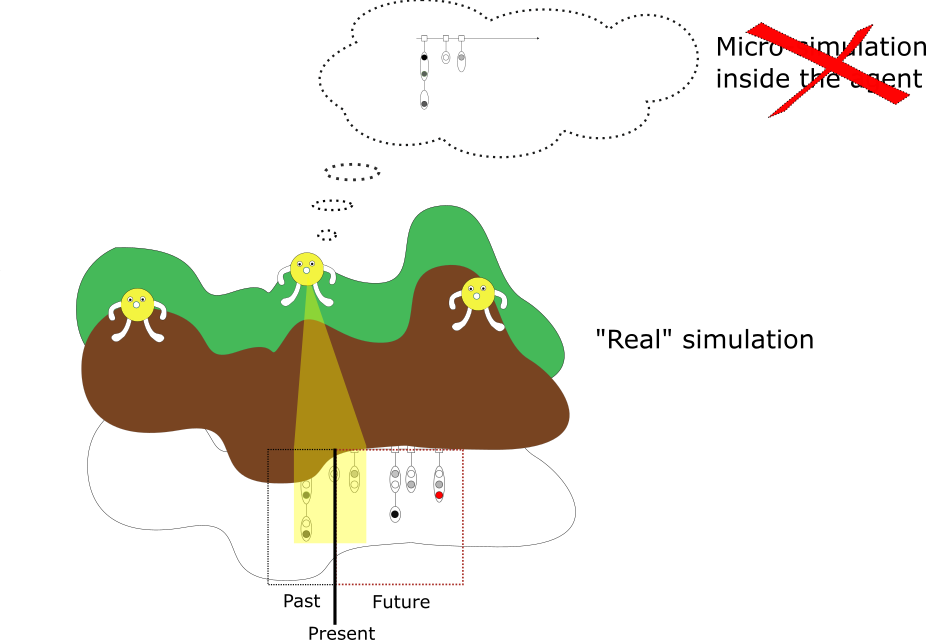
\includegraphics[width=.8\linewidth]{figures/new_anticipation.png}
    \caption{Anticipatory reasoning using the temporal environment perception}
\end{figure}
\note{
\par Nous construisons nos prédiction à partir de la perception des comportements temporels dont l'accès est rendu possible grace à la mise en place de l'environnement temporel. 
\par De plus, contrairement à la plupart des approches classiques qui construisent leur prédisction sur la base des informations passées et présentes, la visibilité sur la dimension future offerte par l'environnement temporel permet à nos agents de prendre en compte les informations temporels positionnées sur le futur.
\par En effet, cette nouvelle dimension d'expression et de partage qui est de nature temporelle permet aux agents de partager leurs projets individuels et de les diffuser sur le collectif. L'analyse prédictive réalisée par les agents se base alors sur la perception de ce nouvel environnement commun, plutôt que par des calculs de simulation reproduits par chacun d'eux.
\par L'état prévisionnel de l'environnement temporel est directement obtenu par perception d'une partie de l'axe temporel contenu dans l'environnement temporel. Cet état prévisionnel est d'autant plus intéressant en ce qui concerne sa précision, car il permet de raisonner sur des informations réelles partagées, au lieu de se baser sur des hypothèses. C'est-à-dire que l'agent n'essaye plus de deviner ce que les autres prévoient de faire comme ce qui est le cas dans la plupart des approches. Dans l'approche que nous proposons, l'agent perçoit les projets individuels des autres agents qui les diffusent sur le collectif, à travers l'environnement temporel.
\par Cela permet à l'agent d'enrichir les informations prises en compte au niveau de son raisonnement anticipatif par des informations sur la dimension future du temps.
}
    
\end{frame}

\begin{frame}{A consideration of the future}{Application}
\par Question agents activity schedule
\par \textbf{Objectives}:
\begin{itemize}
    \item Assess or reassess the feasibility of carrying out an activity
    \item Select the most relevant activity to be carried out
    \item Enrich and bring more precision to the agent's activity planning
\end{itemize}
\begin{figure}
    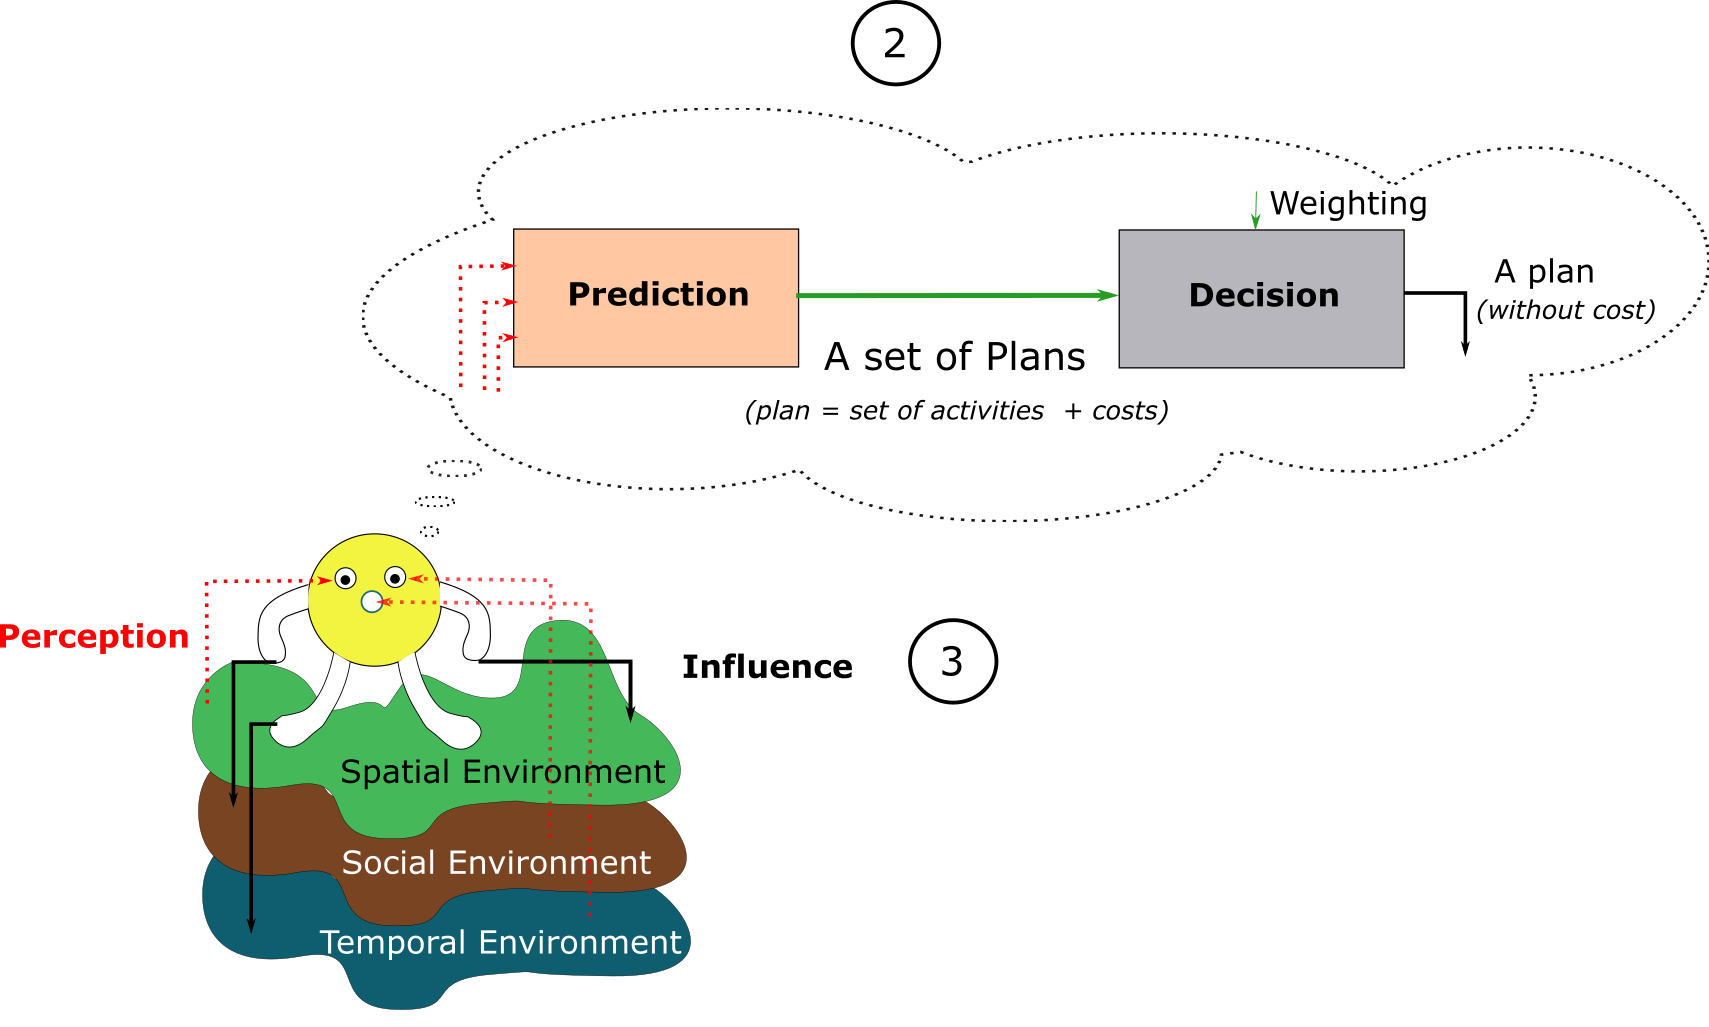
\includegraphics[width=.5\linewidth]{figures/anticipation_cycle.png}
    \caption{Anticipatory reasoning}
\end{figure}
\note{
Dans le raisonnement anticipatif que nous mettons en place au sein des agents du système, nous exploitons les informations que l'agent récolte sous forme de percepts au niveau des différents environnements du système afin de lui permettre de remettre en question son planning d'activités. Les objectifs sont :
\begin{itemize}
    \item évaluer ou réévaluer la possibilité d'exécution d'une activité;
    \item choisir l'activité la plus pertinente à exécuter;
    \item enrichir et apporter plus de précision au planning d'activités de l'agent.
\end{itemize}
\par Le fonctionnement du raisonnement anticipatif consiste en:
\begin{itemize}
    \item L'agent perçoit son contexte d'activation spacial, social et temporel. Plus particulièrement la perception de l'environnement temporel permet de récolter des informations sur le planning d'activité des agents du systèmes, en fonction des horizons temporels (absolues et relatifs) et des règles d'accessibilité. Ce planning contient des informations comportements temporels passées, présentes mais également les projets futurs des agents.
    \item Ces informations sont prises en compte pour générer des prédictions. Ces prédictions prennent la forme d'un ensemble de déclinaison de plan. Ces plans consistement en un enchaînement d'activités avec des coûts. Par exemple: aller travailler à son lieu de travail à 8h avec un cout énergétique de 0.5 sur une échelle de 0 à 1 puis se recharger sur une borne près du lieu de travail avec un coût énergétique de 0 et un coût de longueur prévisionnel de la file de 0.9. ou aller travailler se recharger à 6h sur une borne à proximité du logement du conducteur avec un coût énergétique de 0.1 et un coût en longueur prévisionnel de la file d'attente de 0.1 puis aller travaillet à 8h avec un coût énergétique de 0.5. 
    \item L'agent choisi ensuite le plan le plus pertinent. Pour ce faire, il applique un ensemble de pondération au niveau des coûts. Cela permet de prendre en compte le fait que chaque critère de coût peut avoir une importance différente vis à vis de l'agent et/ou du modélisateur et/ou de l'usager de la simulation. Le choix se base donc sur une minimisation des coûts pondérés. En d'autres termes le plan le plus pertinent est celui donc la somme des coûts pondérée est minimale.
\end{itemize}
}

\end{frame}

\begin{frame}{Temporal reasoning}{Example and implementation}
\begin{columns}
\visible<1->{
\begin{column}{.33\linewidth}
\begin{figure}
    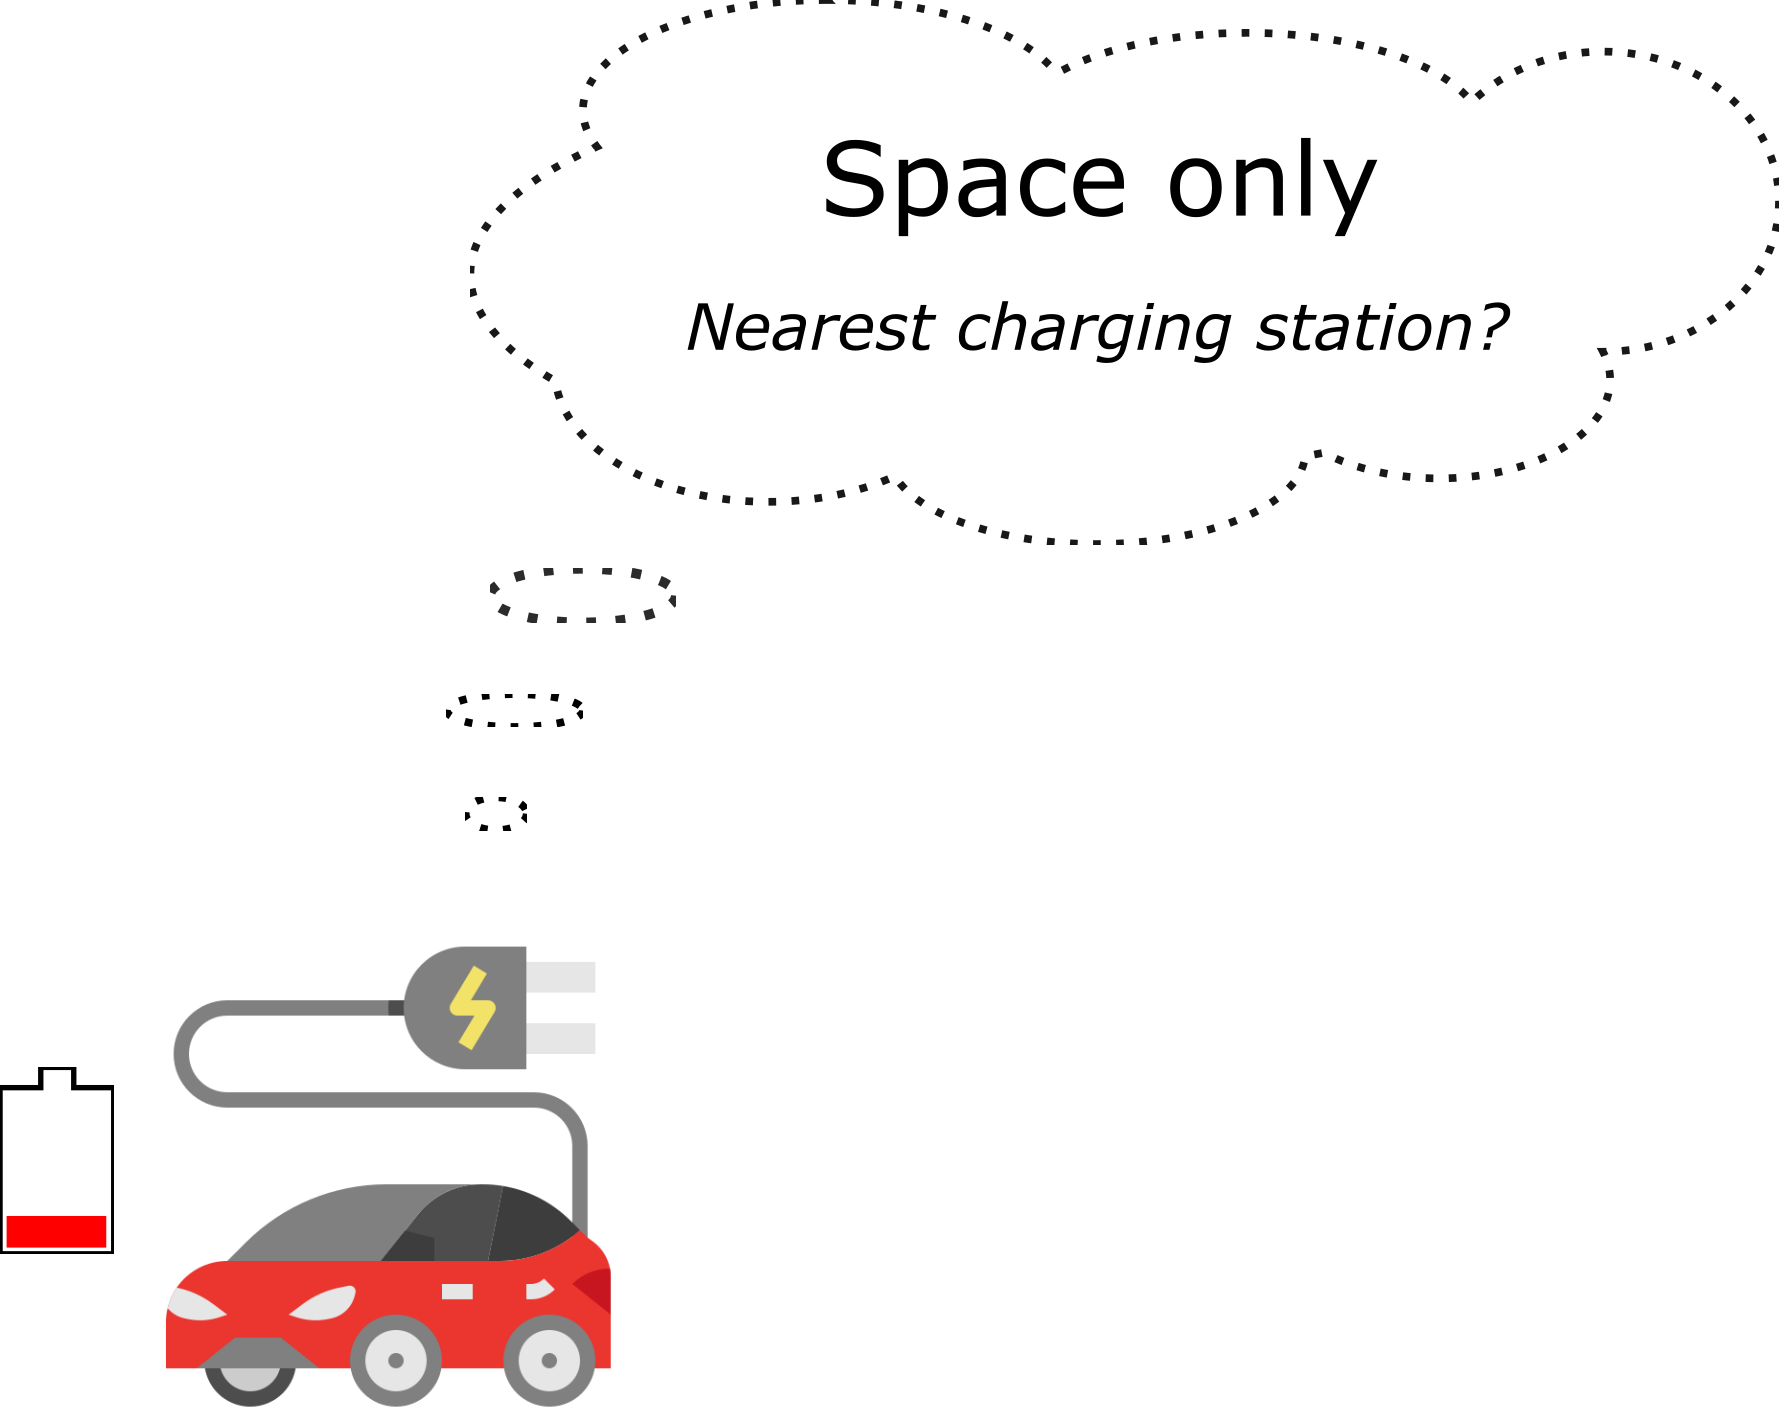
\includegraphics[width=.85\linewidth]{figures/one.png}
   \caption{Classical approach}
\end{figure}
\end{column}
}
\visible<2->{
\begin{column}{.33\linewidth}
\vspace{.3cm}
\begin{figure}
    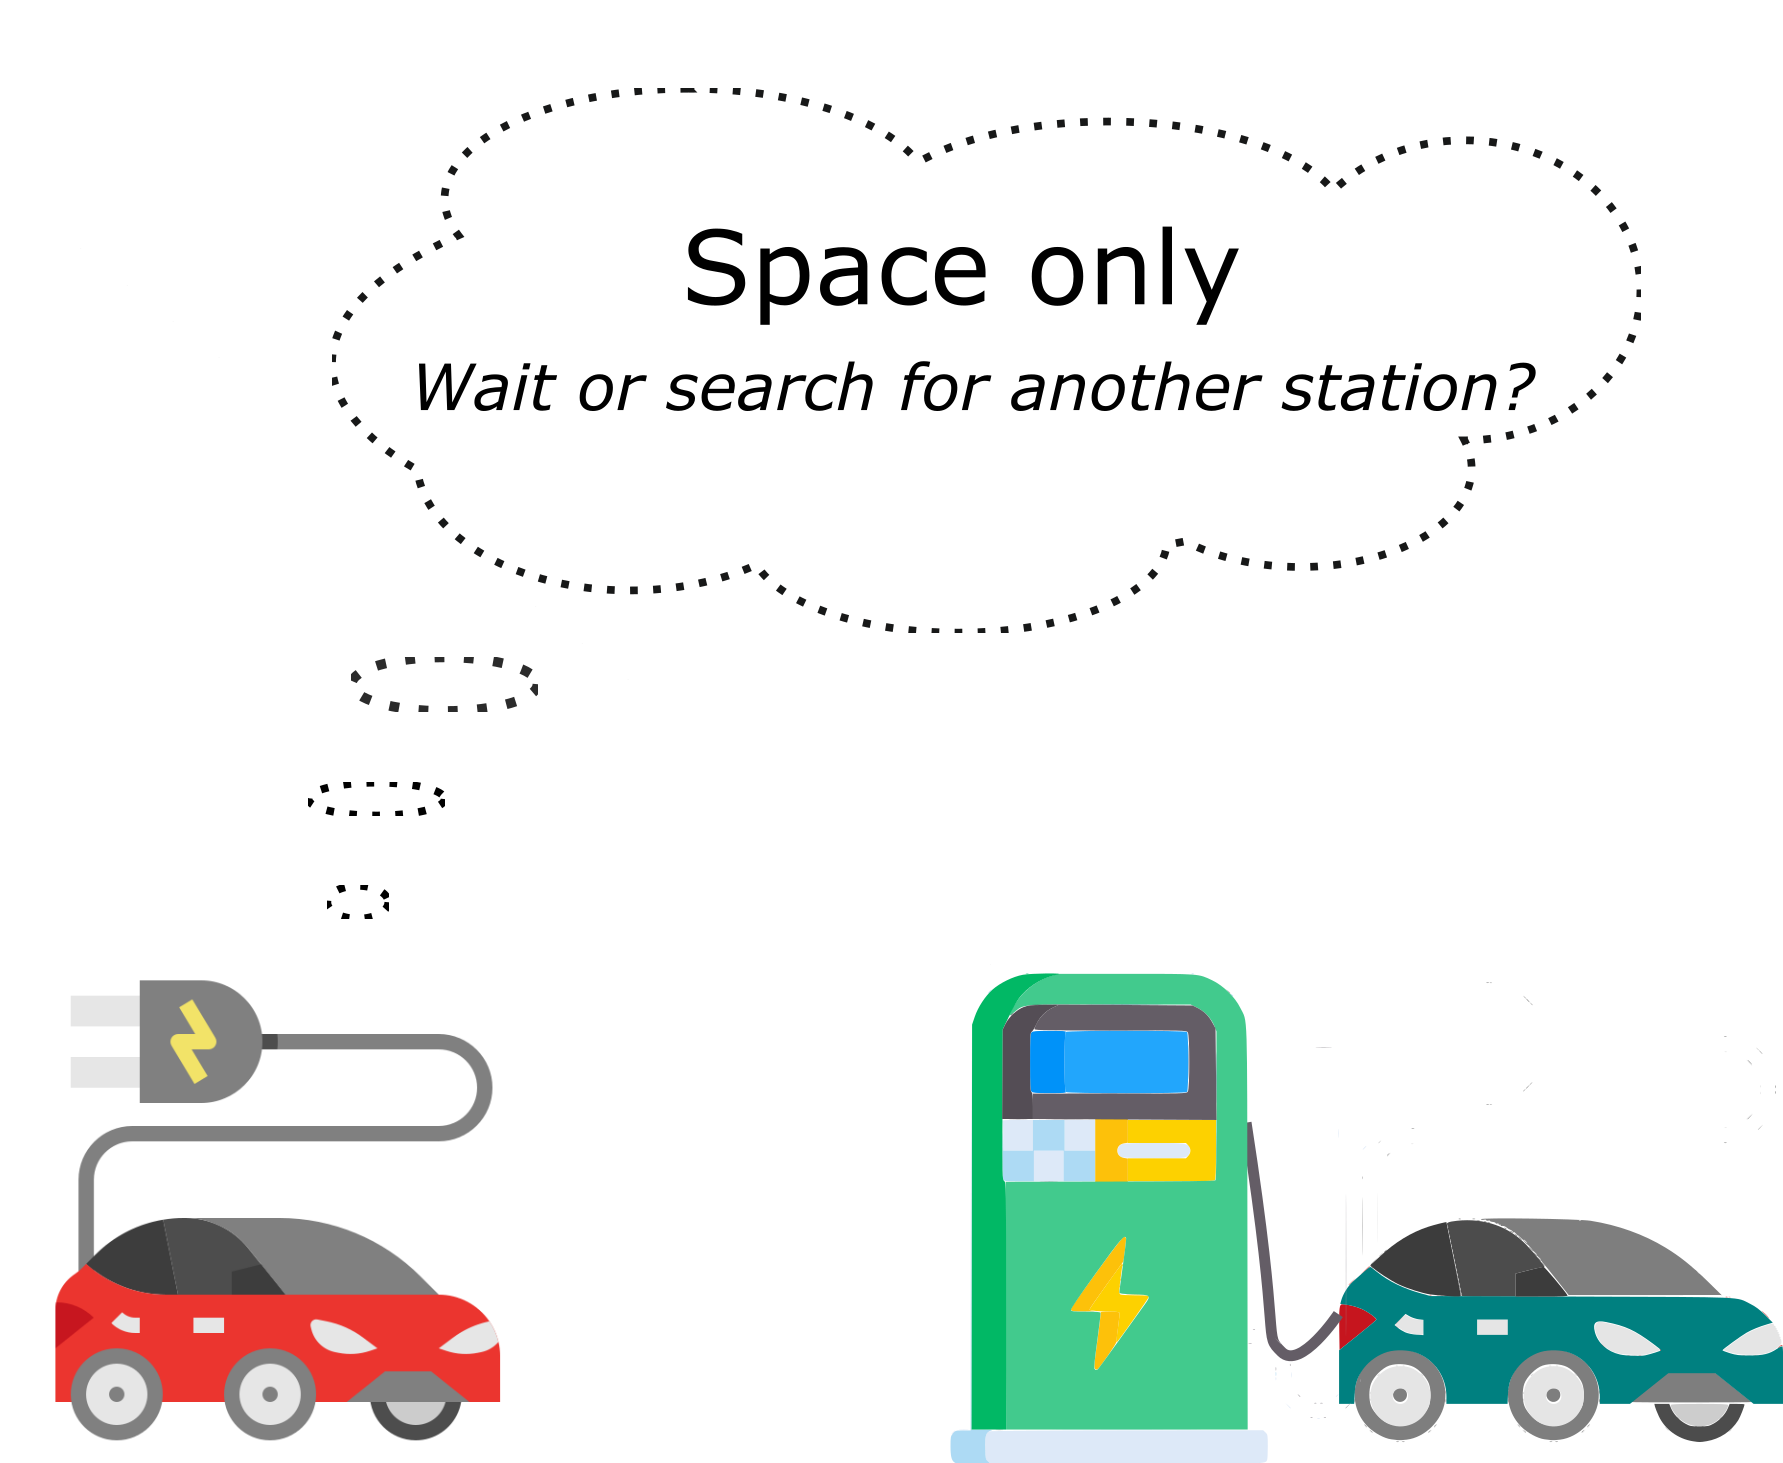
\includegraphics[width=.85\linewidth]{figures/two.png}
\end{figure}
\end{column}
}
\visible<3->{
\begin{column}{.33\linewidth}
\vspace{.4cm}
\begin{figure}
    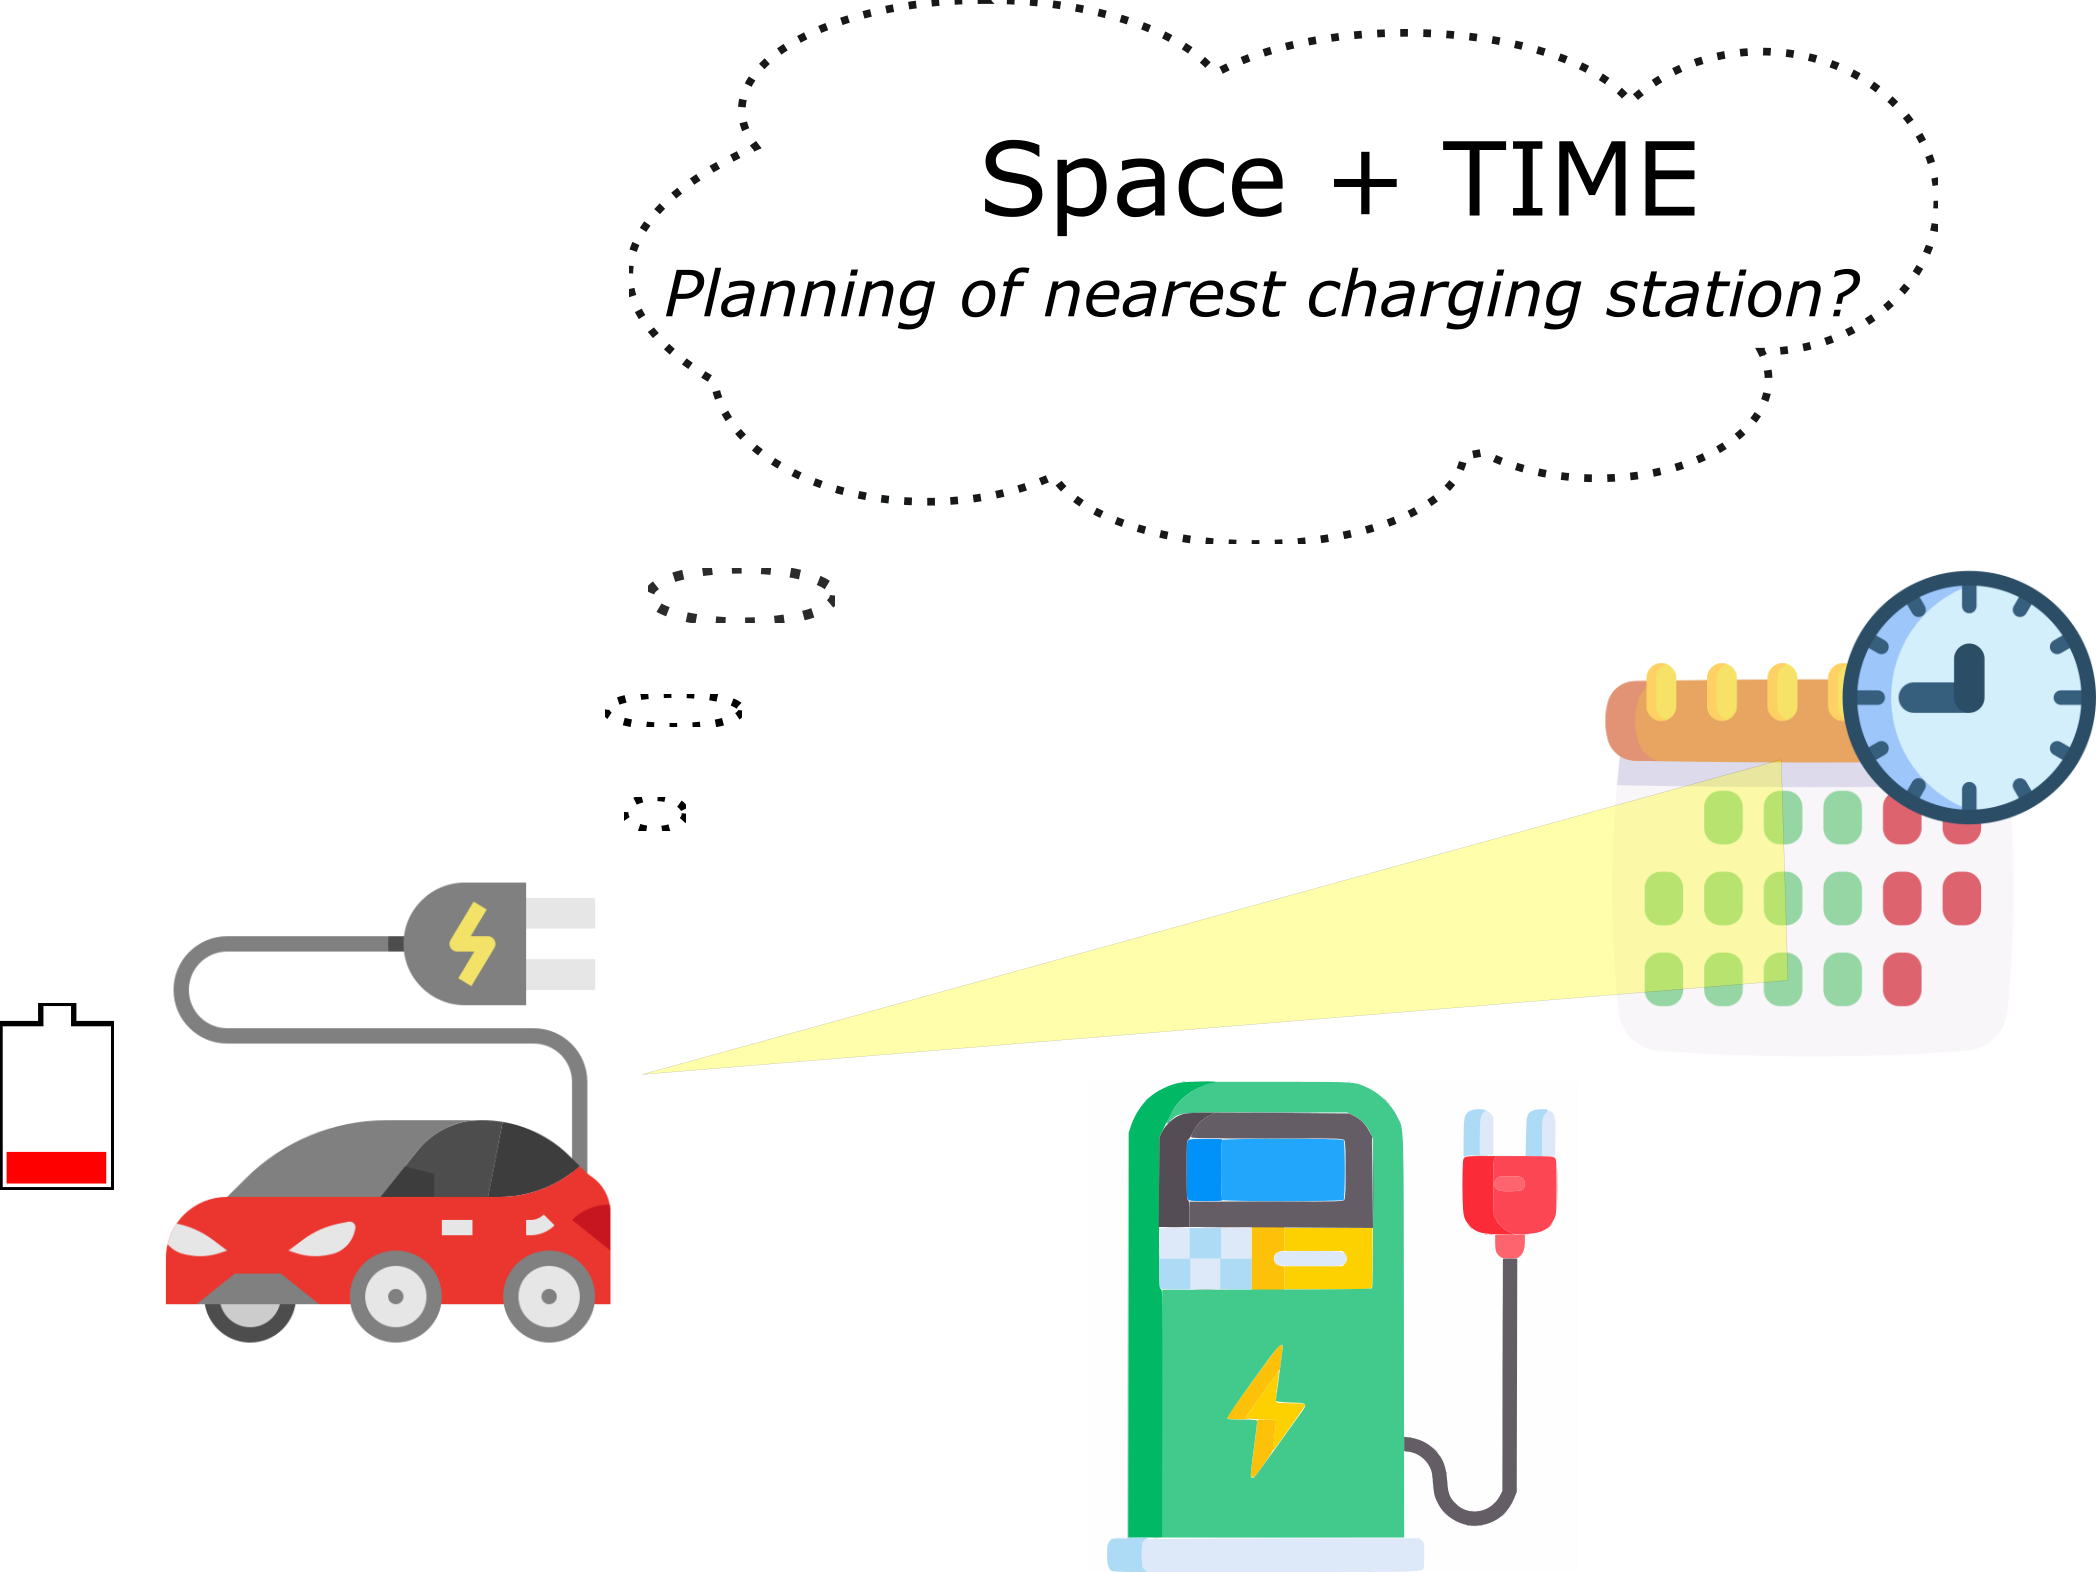
\includegraphics[width=\linewidth]{figures/three.png}
    \caption{Anticipatory reasoning using the temporal environment perception}
\end{figure}
\end{column}
}
\end{columns}


\note{
\par Avant l'intégration de notre contribution, le raisonnement de l'agent se basait uniquement sur le spatial. Par exemple, lorqu'un conducteur de véhicule électrique détecte un niveau de batterie faible de son véhicule, il se met à cherche la borne de recharge la plus proche spatialement et se déplace vers cette borne. Une fois arrivé, si la borne est libre, il s'y branche pour se recharger, sinon il se met dans la file d'attente ou cherche une autre borne libre et répète le processus. 
\par Une autre version un peu plus évoluer de ce système consiste à intéroger les bornes de recharges à proximité spatiales de leur état et de choisir d'aller se recharger vers celle qui est libre. Cependant, rien ne garantit que, le temps d'arriver à cette borne, cette dernière sera encore disponible. Il se peut que d'autres agents aient aussi eu l'idée d'aller s'y recharger et y sont arrivés plus tôt.
\par L'intégration de notre première contribution permet à l'agent d'avoir une visibilité sur le planning d'activité des autres agents du système. Ainsi, le conducteur de véhicule électrique peut avoir une visibilité sur une partie du planning prévisionnel de la borne de recharge. Il peut donc connaître à l'avance si un autre conducteur a prévu de se recharger sur la même borne sur le même créneau. Il aura la visibilité sur la longueur prévisionnelle de la file d'attente. Tout cela lui permet de raisonner sur un espace temporel plus large et de  d'anticiper, avant même d'effectuer le déplacement si sa décision lui semble pertinente vis à vis de ses objectifs ou s'il doit remettre en question une partie de son comportement temporel prévisionnel. 
}
    
\end{frame}
\section{Conclusion}
\begin{frame}{Summary}
\par An approach that allows agents to reason equitably on the basis of spatial, social and temporal dimensions
\vspace{.4cm}
\par How to offer agents visibility on the temporal dimension as it is already the case for the spatial and social dimension?
\par \alert{$\rightarrow$ The temporal environment} allows the agent to share, store and perceive temporal information
\par \alert{$\rightarrow$ The Agent-Group-Role-Environment-Time (AGRET)} allows the consideration of the 3 dimensions in the same way
\medbreak
\par How to take into account information about the future in the agent's anticipatory reasoning?
\par \alert{$\rightarrow$ The temporal environment} offers agents accessibility on the future dimension of time
\vspace{.4cm}
\end{frame}

\begin{frame}{Summary}
\par \textbf{Multi-agent level}: 
\begin{itemize}
    \item Evolution of multi-agent simulation to  consider the temporal dimension in the same way as the spatial and the social dimension
    \item Optimisation of the agents behaviours choice relevance
\end{itemize} 
\medbreak
\par \textbf{Smart city level}: 
\begin{itemize}
    \item Taking into account the 3 dimensions of the territorial system (space, organization, time)\footnote{ROLLAND-MAY, Christiane. Évaluation des territoires: concepts, modèle, méthodes. Hermès science publications, 2000.}
    \item Generate higher levels of user engagement: exchange and processing of information 
\end{itemize}
\note{
L'intelligence dont il est sujet dans la ville intelligente est notamment une forme d'intelligence participative qui émerge des interactions entre les citoyens et le système.
}
    
\end{frame}

\begin{frame}{Further work}
\par Are there other non-time-constrained environments?
\par \alert{$\rightarrow$ Observation environments for example}
\vspace{1cm}
\par Could social media be exploited to a greater extent?
\par \alert{$\rightarrow$ Define more advanced visibility and accessibility rules}
\begin{itemize}
    \item Networks: circle of friends, social groups, etc.
\item Popularity: reactions, like, etc.
\end{itemize}

\note{
\par Les contributions de cette thèse donnent lieu à plusieurs pistes de recherches. Nous en sélectionnons quelques unes qui nous paraissent particulièrement interessantes.
\par L'introduction du nouveau type d'environnement de nature temporel nous a fait prendre conscience de l'existance d'au moins deux types d'environnements : les environnements contraints par le temps comme l'environnement spatial et l'environnement social. Les environnements non-contraints par le temps comme l'environnement temporel. Nous nous posons alors la question sur la possibilité d'existance d'autres environnements non contraints par le temps, des environnements, des méta-environnement qui évoluent hors du temps. Nous pensons par exemple aux environnements d'observation dont le fonctionnement nous semble sortir du cadrade limité par le temps.
\par Une autre perspective qui nous semble interessante vis à vis du cadre des systèmes multi-agents et d'une manière plus générale, vis-à-vis des smart cities, consiste en l'exploitation des réseaux sociaux.
\par Une utilisation consisterait à définir des règles de visibilité et d'accessibilité en fonction des réseaux sociaux. Nous citons notamment deux notions utilisées dans les réseaux sociaux qui nous semble interessantes:
\begin{item}
\item Les réseaux d'accointances : cercle d'ami, groupe sociaux
\item La notion de popularité : les réactions, le pouce "j'aime" qui permet de qualifier l'importance d'une information.
\end{item}
}
    
\end{frame}

\begin{frame}{Further work}
\begin{figure}
    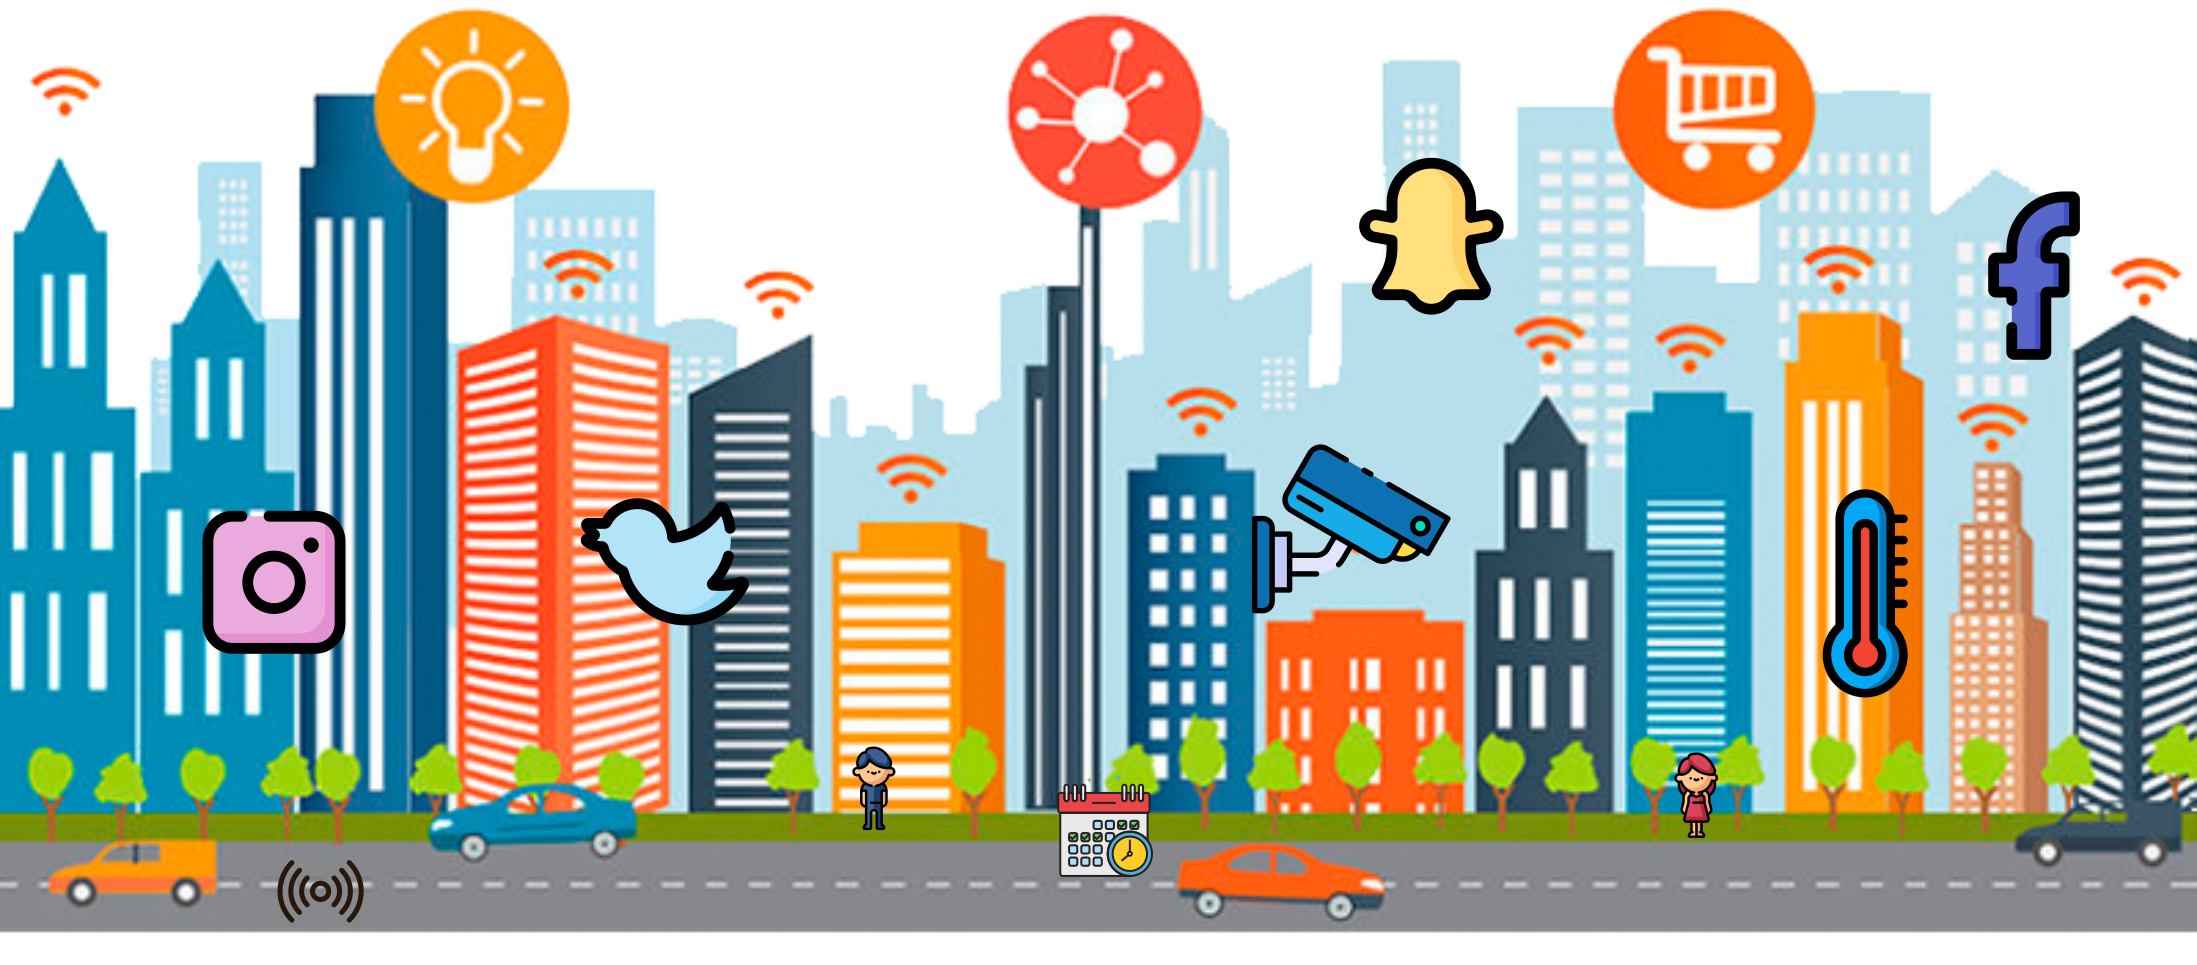
\includegraphics[width=\linewidth]{figures/smartcity.png}
\end{figure}
\centering
Promote the emergence of standards and protocols for smart cities
%reboucler sur les smart cities
\note{Les réseaux sociaux sont notamment très fortement utilisées actuellement dans le villes. Son exploitation devrait nous permettre d'optimiser la participation et l'engagement du citoyen au niveau du système, favorisant encore plus l'émergence des standards et protocoles propres aux villes intelligente}
\end{frame}
\begin{frame}[allowframebreaks]{References}

  \nocite{*}
  \bibliography{demo}
  \bibliographystyle{abbrv}

\end{frame}

%\section{Introduction}

%\subsection{Background (Chapter 1)}
%\begin{frame}{General Background}
\begin{columns}
\begin{column}{.48\linewidth}
\begin{block}{\visible<4->{Pressure on resources management}}
\begin{itemize}
    \visible<1->{\item Growing urbanisation}
    \visible<2->{\item Economical crises}
    \visible<3->{\item Environmental crises}
\end{itemize}
\end{block}
\end{column}
\begin{column}{.48\linewidth}
\visible<6->{
\begin{block}{\visible<6->{Contributions of ICT}}
\begin{itemize}
    \visible<7->{\item Changes in multiple level}
    \visible<8->{\item Digitalization}
    \visible<9->{\item Importance of information}
\end{itemize}
\end{block}
}
\end{column}
\end{columns}
\vspace{.3cm}
\visible<5->{
\begin{figure}
\centering
	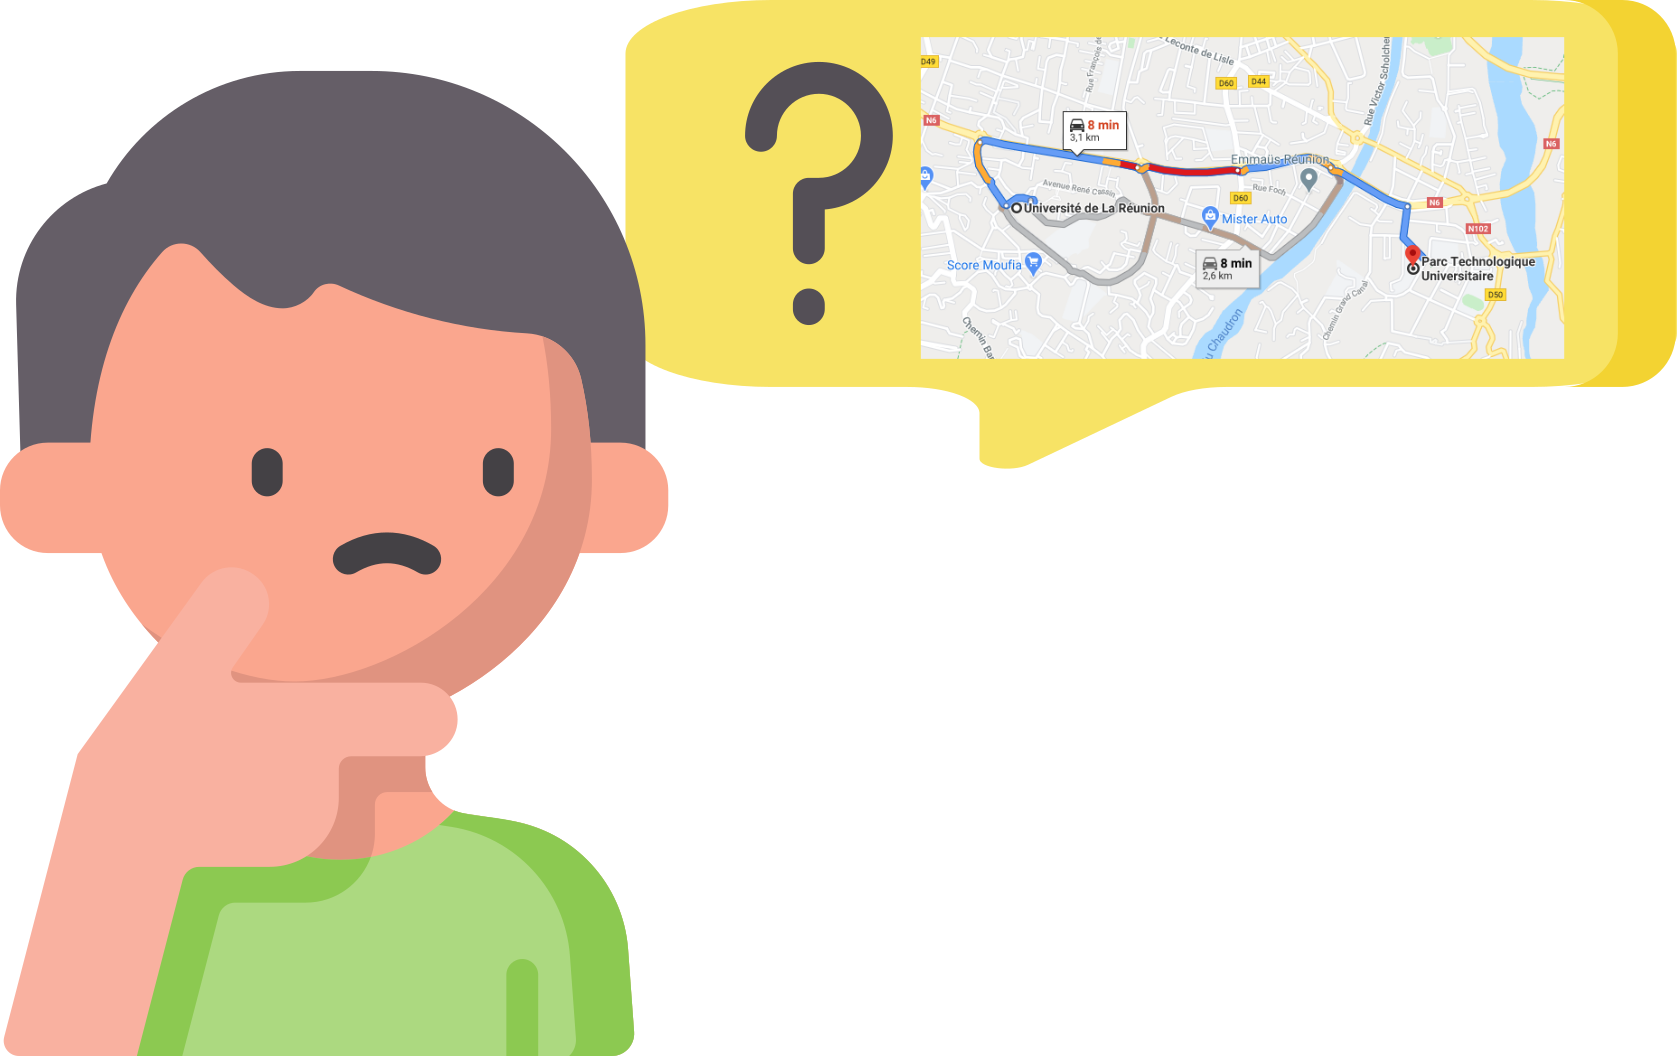
\includegraphics[width=.2\textwidth]{figures/question.png}
\end{figure}
}
\vspace{.3cm}
\centering \visible<10->{\alert{\huge{SMART CITY}}}
\note{
Nous faisons face à un phénomène d'urbanisation croissante accompagné de différentes crises économiques et environnementales qui engendrent d'autres crises comme la crise sanitaire que nous affrontons actuellement. Ces crises mettent une énorme pression sur la structure des villes et sur la gestion des ressources. Nous sommes alors contraints à chercher des solutions pratiques, techniques à ces différents problèmes, tout en prêtant uneattention particulière à l’environnement et au développement durable. En parallèle à cela, nous assistons, depuis ces dernières décennies à la montée en puissance des TIC qui contribue fortement à de grands changements au niveau de la ville, sur tous ses aspects : économique, culturel, transport, communication, etc. Les villes deviennent de plus en plus numériques et basées sur l’information.  Ces tendances ont conduit à la popularité du concept de ville intelligente ou smart city qui est considéré comme une solution aux problèmes évoquées précédemment.}
\end{frame}

%%%%%%%%%%%%%%%%%%%%%%%%%%%%%%%%%%%%%%%%%%%%%%%%%%%%%%%%%%%%%%%%%
\begin{frame}{General Background}{Smart City}
\begin{columns}
\begin{column}[l]{.48\linewidth}
\begin{figure}
	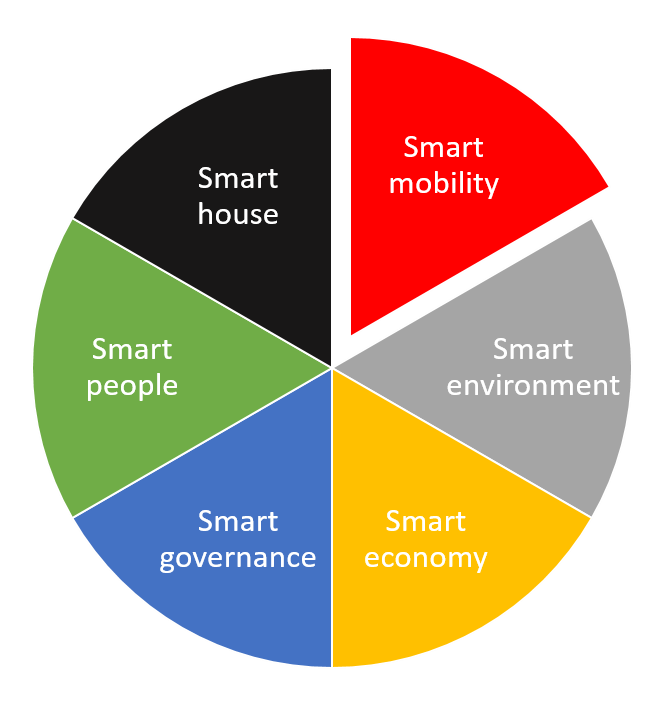
\includegraphics[width=\textwidth]{figures/smart_city.png}
\end{figure}
\end{column}
\begin{column}{.48\linewidth}
\visible<2->{\begin{block}{Criteria}
\begin{itemize}
    \item A bottom-up approach
    \item A more inclusive approach to citizens
    \item A participatory intelligence that emerges from the interactions between citizens and the system
\end{itemize}
\medbreak
\centering
\visible<3->{\alert{MULTI-AGENT SIMULATION}}
\end{block}}
\end{column}
\end{columns}
\note{\only<1>{Il n'existe pas encore de standard permettant de définir ce qu'est une ville intelligente. Plusieurs définitions peuvent se retrouver dans la littérature, mettant en valeur une ou plusieurs aspects de la ville. Celle que nous pensons la plus complète est celle de Giffinger. Giffinger défini une ville intelligente comme une ville qui est performante en 6 caractéristiques : l'environnement, l'économie, la mobilité, l'habitat, la gouvernance et le citoyen. Nous nous intéressons particulièrement à la mobilité intelligente. Cependant, nous pensons que nos solutions sont assez génériques pour être applicable aux autres domaines. Je reviendrai plus en détail sur notre cadre applicatif autour de la mobilité intelligente plus tard.}

\only<2>{Contrairement à beaucoup d'autres définitions qui ont tendance à négliger la place du citoyen ou aux mieux à les prendre en compte de façon marginale: en tant que consommateurs, dont les habitudes sont scrutées et régentées par des systèmes techniques, nous pensons que les citoyens occupent une place centrale dans la mise en oeuvre d'une ville intelligente. L'intelligence dont il est sujet ici est notamment une forme d'intelligence collective qui émerge des interactions entre le citoyen et le système. Dans ce contexte, les nouveaux outils du numérique facilitent grandement la participation des citoyens à l'élaboration des politiques, à la planification, etc. Ces citoyens échangent des informations et adoptent des comportements qui tendent à satisfaire des objectifs collectifs.}

\only<3>{L'approche multi-agent est une approche prometteuse permettant de modéliser ces types de systèmes. C'est une approche ascendante. Elle fait l'objet depuis longue date de recherches en intelligence artificielle distribuée. Appliqués au système de la ville, les sma permettent de décomposer cette dernière en plusieurs sous-ensembles plus simples, gérés par plusieurs entités autonomes, sociales, réactives et pro-actives appelées agents. Les sma permettent également de modéliser la non-linéarité et favorisent l’émergence des normes et des protocoles nécessaires pour les villes intelligentes.
\medbreak
Le domaine des sma mobilise des scientifiques issus majoritairement de l’informatique, des sciences cognitives et des systèmes complexes. Il produit un large spectre de solutions dans des champs d'applications tels que le développement de systèmes informatiques décentralisés, la résolution collective de problème, le développement de systèmes médiatisés ou encore la simulation de phénomènes complexes. C'est ce dernier champ d'application qui nous intéresse dans le cadre de nos travaux. Nous nous focalisons particulièrement sur les modèles de simulation multi-agent. Ces modèles de simulation servent à analyser le fonctionnement de scénario choisi, afin de déduire des enseignements pratiques de gestion opérationnelle dans le cadre de la conception et de la planification de villes intelligentes.}
}
\end{frame}

%%%%%%%%%%%%%%%%%%%%%%%%%%%%%%%%%%%%%%%%%%%%%%%%%%%%%%%%%%%%%%%%

\begin{frame}{Application Context}
\begin{itemize}
    \item Collective Adaptative System working group
    \item Multi-agent System :
    \begin{itemize}
        \item Focus on multi-agent simulation
        \item Hybrid approaches
    \end{itemize}
\end{itemize}


\note{
Cette thèse s’inscrit dans la continuité des travaux étudiés précédemment par le groupe de travail SCA du LIM. Notre équipe de recherche est spécialisée dans le paradigme des SMA, avec un accent particulier sur les aspects de simulations. Néanmoins, la politique actuelle de l’équipe s’oriente plus vers les approches de type hybrides. Cela veut dire qu’elle ne s’intéresse plus uniquement à la simulation, mais aussi à l’application dans un environnement réel. 
}
\end{frame}
%%%%%%%%%%%%%%%%%%%%%%%%%%%%%%%%%%%%%%%%%%
\begin{frame}{Application Context}
\begin{columns}
\begin{column}{.10\linewidth}
\begin{figure}
	
\includegraphics[width=\textwidth]{assets/icl.png}
\end{figure}
\begin{figure}
	
\includegraphics[width=\textwidth]{assets/saintDenis.png}
\end{figure}
\end{column}
\begin{column}[l]{.68\linewidth}
\begin{itemize}
    \item Multi-agent simulation of smart city and smart island : Smart mobility
    \item Multi-agent simulation of electric vehicle travel flows:
    \begin{itemize}
        \item SkuadCityModel
        \item SmartCityModel
    \end{itemize}
\end{itemize}
\vspace{1cm}
\textbf{Problem : } management of shared resources, limited in space and time
\end{column}
\end{columns}
\note{
Un des sous-thèmes développés consiste en l’application des simulations multi-agent dans le domaine des villes intelligentes et des îles intelligentes. Il s’agit d’un domaine en émergence dans notre équipe et sur lequel nous travaillons en collaboration avec des chercheurs de l'ICL et avec la mairie de Saint-Denis, La Réunion. Les problématiques abordées sont en lien avec la mobilité intelligente. Nous appliquons notre approche sur un modèle de simulation multi-agent de flux de déplacement de véhicules électriques sur un territoire que nous développons au sein même de notre équipe. Ce modèle s’appelle SkuadCityModel. Il se base sur un modèle développé par les chercheurs de l’ICL appelé SmartCityModel, sur lequel nous avons également contribué et qui a fait l'objet de deux contributions. Les problématiques abordées dans le cadre de cette thèse découlent des limites détectées lors de ces expérimentations. Nous nous intéressons notamment à des problématiques liées à la gestion de ressources partagées et limitées dans l’espace et dans le temps. Cette dernière fait partie des problèmes à l’origine même de la création du concept de ville intelligente. L’exemple sur lequel nous nous basons est celui du rechargement des véhicules électriques avec des bornes de recharge publiques.}
    
\end{frame}


%%%%%%%%%%%%%%%%%%%%%%%%%%%%%%%%%%%%%%%%%%
\begin{frame}{Application Context}{The example of the electric vehicle flow simulation}
\begin{columns}
\begin{column}{.48\linewidth}
\begin{figure}
	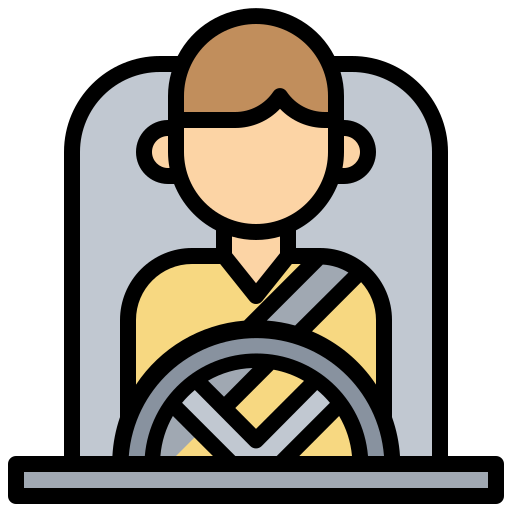
\includegraphics[width=.7\textwidth]{figures/driver.png}
\end{figure}
\centering {\Large Driver}
\end{column}
\begin{column}{.48\linewidth}
\begin{figure}
	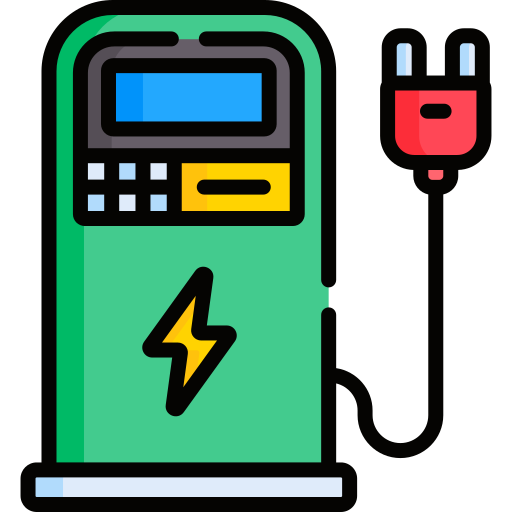
\includegraphics[width=.7\textwidth]{figures/electric-charge.png}
\end{figure}
\centering {\Large Charging point}
\end{column}
\end{columns}
\note{La recharge de véhicules électriques implique principalement deux entités : le conducteur de voiture électrique et la borne de recharge. Ces deux entités sont autonomes et indépendantes.}
\end{frame}


%%%%%%%%%%%%%%%%%%%%%%%%%%%%%%%%%%%%%%%%%%%%%%%%%%%%%%%%%%%%%%%%%%%%%%%%%%%%%%%
\begin{frame}{Application Context}{The example of the electric vehicle flow simulation}
\alt<1-6>{
\begin{block}{Driver}
\begin{columns}
\begin{column}{.18\linewidth}
\begin{figure}
	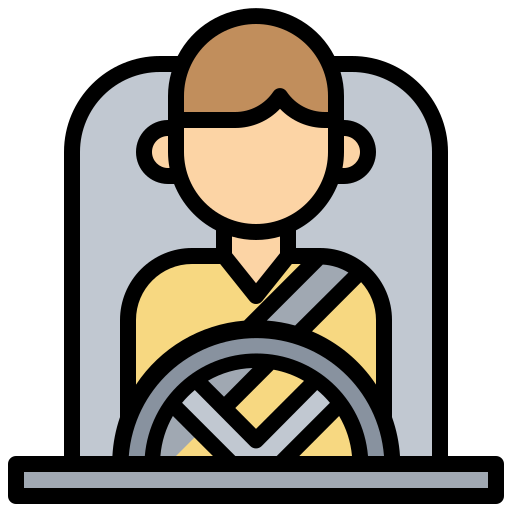
\includegraphics[width=\textwidth]{figures/driver.png}
\end{figure}
\end{column}
\begin{column}{.78\linewidth}
\begin{itemize}
    \visible<2->{\item Own a schedule composed of daily life activities that require travel}
    \visible<3->{\item The activities are situated in time and space}
    \visible<4->{\item \textbf{Main objective}: to accomplish all his planned activities}
    \visible<5->{\item \textbf{Main constraint}: recharging}
    \visible<6->{\item \textbf{Main strategy}: optimizing recharging
    \begin{itemize}
        \item Choosing the right time
        \item Minimise the recharging duration
    \end{itemize}
    
    }
\end{itemize}
\end{column}
\end{columns}
\end{block}
}{
\begin{block}{Charging point}
\begin{columns}
\begin{column}{.18\linewidth}
\begin{figure}
	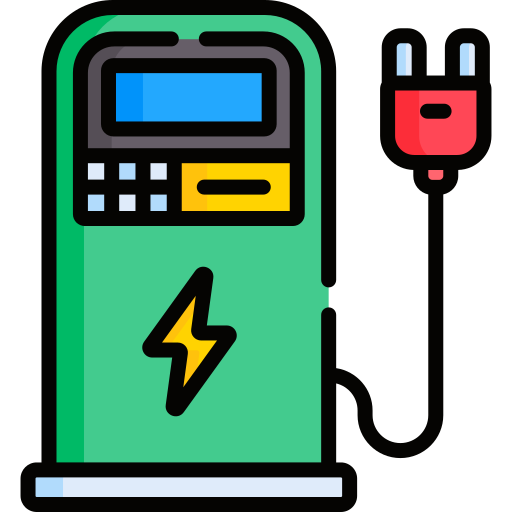
\includegraphics[width=\textwidth]{figures/electric-charge.png}
\end{figure}
\end{column}
\begin{column}{.78\linewidth}
\begin{itemize}
    \visible<7->{\item Limited number}
    \visible<8->{\item The availability is not guaranteed at any time or place}
    \visible<9->{\item \textbf{Main objective}: optimize its occupancy rate}
    \visible<10->{\item \textbf{Main constraint}: queue length}
    \visible<11->{\item \textbf{Main strategy}: optimize the distribution of electric vehicle recharging in its queue}
\end{itemize}
\end{column}
\end{columns}
\end{block}
}

\note{
\alt<1-6>{Dans SkuadCityModel, comme dans la réalité, un automobiliste possède un planning d'activité plus ou moins défini à l'avance. Ce planning se compose de différentes activités de la vie quotidienne nécessitant des déplacements : aller travailler, aller se divertir, rentrer chez soi ou faire ses courses. Ces activités sont situées dans le temps et dans l'espace. Cela revient à dire qu'à chaque activité, nous pouvons associer une composante spatiale (le conducteur va travailler à un endroit précis), et une composante temporelle (le conducteur part travailler à une heure précise).
\medbreak
L'objectif principal de l'automobiliste est d'accomplir l'ensemble des activités qu'il a prévues dans son planning. Pour ce faire, il se déplace en utilisant son véhicule électrique. Cependant, ce dernier possède une autonomie de batterie limitée. Par conséquent, le rechargement devient une contrainte. Le conducteur optimise alors au maximum le rechargement, de manière à ce qu'il puisse respecter son planning. Cette optimisation consiste à choisir le bon moment pour se recharger et à minimiser la durée du rechargement. Cette durée de rechargement inclut la durée d'attente au niveau de la borne de recharge.}
{
Le nombre de bornes de recharge est limité. En France par exemple, le ratio de véhicules par point de charge est de 5,7. Ce nombre peut varier en fonction de la situation géographique de la borne. Par conséquent, la disponibilité d'une borne n'est garantie ni à tout moment ni à tout endroit, car d'autres véhicules peuvent l'utiliser. Son objectif principal est d'optimiser son taux d'occupation. 
Cette situation a des répercussions tant au niveau de la borne qu'au niveau de l'automobiliste. Pour la borne, une forte demande de rechargement augmente le nombre de véhicules en attente (la longueur de la file d'attente). Elle est donc contrainte à trouver un moyen de bien gérer la répartition du rechargement des véhicules dans sa file d'attente. }
}
\end{frame}

\begin{frame}{Application Context}{The example of the electric vehicle flow simulation}
\textbf{Problem}: Management of a shared and limited resource in space and time.
\begin{itemize}
    \item lack of information for more precise reasoning.
    \item the charging point is not aware of the state of each vehicle or the schedule of the driver.
    \item no support is provided so that the driver can access all the information held by the charging point.
\end{itemize}

\note{ Ceci illustre donc un problème de gestion de ressources partagée et limitée dans l'espace et dans le temps.
\par La borne est contrainte à trouver un moyen de bien gérer la répartition du rechargement des véhicules dans sa file d'attente. Cependant, il s'agit d'une tâche difficile, car elle n'a connaissance ni de l'état de chaque véhicule ni du planning de l'automobiliste qui le conduit. Elle ne connaît donc pas la disponibilité de leur conducteur. Du côté de l'automobiliste, l'occupation des bornes et l'augmentation de la longueur de la file d'attente multiplient le temps nécessaire pour effectuer le rechargement. Elle réduit également le nombre de créneaux de rechargement disponibles. Cela constitue une contrainte qui pourrait perturber son planning et l'empêcher d'atteindre son objectif. L'automobiliste devra donc prendre en compte les informations concernant le planning et l'état de la borne dans ses décisions. Cependant, tout comme pour la borne, aucun support n'est prévu pour que l'automobiliste puisse accéder à la totalité des informations qui sont détenues par la borne.}
    
\end{frame}
%\subsection{Problem (Chapter 1)}
%\begin{frame}{Problems}
\begin{block}{Management of a shared and limited resource in space and time}
\begin{itemize}

\item The need for \alert{interaction support} to exchange spatial, social and temporal information

\item The need for \alert{reasoning} that takes into account the spatial dimension, the temporal dimension and the social dimension

\end{itemize}
\end{block}

\note{Cet exemple fait alors ressortir deux besoins sur lesquels nous apportons notre contribution :
\begin{itemize}
    \item Le besoin en support interaction spatial, social, et temporel
    \item Le besoin en raisonnement qui prenne en compte les informations partagées par le biais du support interaction. Ces informations concernent les trois (3) dimensions : spatiale, temporelle et sociale .
\end{itemize}}
\end{frame}

\begin{frame}{Contributions}
Our contributions deal with the 2 dimensions of time:
\begin{itemize}
    \item \textbf{The time representation}: topology, structure as well as the approaches that allow to model it;
    \item \textbf{The temporal reasoning}: manipulation of these representations in order to make calculations, to conduct reasoning based on them. \textbf{Anticipation}
\end{itemize}	
    
\note{Pour répondre à ces deux besoins, nous nous concentrons particulièrement sur la dimension temporelle dans les SMA. Nos contributions portent sur deux aspects de cette dimension temporelle : la représentation du temps et le raisonnement temporel. 
\par La représentation du temps peut être implicite ou explicite et traite de sa topologie, de sa structure ainsi que des approches qui permettent de le modéliser. 
Le raisonnement temporel quant à lui est lié à la manipulation de ces représentations afin d'effectuer  des calculs, conduire des raisonnements à partir de celles-ci. En intelligence artificielle, le raisonnement temporel équivaut à un raisonnement sur ce qui change au cours du temps. Cela correspond au raisonnement sur le temps. Cependant, il convient également de souligner l'existence dans des domaines spécifiques et spécialisés (systèmes temps réel, parallélisme, etc.) d'un raisonnement dans le temps qui s'intéresse au temps nécessaire pour le calcul. Cela ne nous intéresse pas puisque le temps de calcul n'est pas la préoccupation primordiale des systèmes sur lesquels nous nous penchons. Différents problèmes très souvent issus du milieu industriel sont associés au raisonnement temporel : la planification, l'ordonnancement de tâches, le suivi de processus, le diagnostic, la prédiction. Dans notre contexte, nous choisissons de nous focaliser sur l'anticipation.

Avant d’entrer plus en détails dans ces contributions, pour une meilleure compréhension, je vais expliquer brièvement comment le temps est pris en compte actuellement dans les SMA
}
\end{frame}

\begin{frame}{Taking time into account in multi-agent simulation}
\visible<1->{
\begin{block}{Multi-agent simulation model}
\visible<2->{Schematic representation of reality with a view to studying and understanding it}
\begin{itemize}
    \visible<3->{\item A set of agents}
    \begin{itemize}
        \visible<11->{\item Behavioural cycle: perception, deliberation, action/influence}
    \end{itemize}
    \visible<4->{\item An environment}
    \begin{itemize}
        \visible<7->{\item spatial and/or social}
        \visible<8->{\item contain spatial and social activation contexts data}
    \end{itemize}
    \visible<5->{\item A set of objects}
    \visible<6->{\item A set of relation}
        \begin{itemize}
        \visible<9->{\item Agents act or exert an influence on their environment}
        \visible<10->{\item Agents perceive their environment}
    \end{itemize}
\end{itemize}
\end{block}
}
\visible<1->{
\begin{block}{Simulation platform}
\end{block}
}

\note{Une simulation multi-agents peut se diviser en deux grandes parties: la plateforme de simulation ou simulateur, le modèle de simulation. Le modèles de simulation proposent une représentation schématique de la réalité en vue de l’étudier, de la comprendre. Un modèle simulation multi-agent est  composé d’un ensemble d’entités autonomes, que l’on appelle agents, situés dans un certain environnement et interagissant selon certaines relations. D’une manière plus formelle Ferber caractérise un système multi-agent par un environnement (E), un ensemble d’objets (O) situés dans E. Ces objets peuvent être perçus, créés, détruits et modifiés par les, un ensemble d’agents (A), qui sont des objets particuliers, lesquels représentent les entités actives du système, un ensemble de relations (R) qui unissent des objets (et donc des agents) entre eux.
\par Dans la plupart des modèles, l’environnement est soit un environnement spatial, soit un environnement de communication dont un cas particulier est l’environnement social. Ces environnements contiennent les données relatives aux contextes d’activation spatiales et sociales de l’agent. La relation entre l’agent et son environnement se traduit par le fait que l’agent agit ou exerce une influence sur son environnement et le perçoit. 
\par Le cycle comportemental classique d’un agent se résume alors en trois phases: une phase de perception où il récolte des informations contenues au niveau de l’environnement, une phase de délibération où l’agent active son processus de raisonnement et choisi un comportement à exécuter en fonction des percepts qu’il aura récolté et de son état interne et une phase d'action ou d’influence où l’agent agit ou essaie d’agir sur son environnement.
}
\end{frame}

\begin{frame}{Taking time into account in multi-agent simulation}
\begin{block}{Multi-agent simulation model}
\end{block}
\begin{block}{Simulation platform}
\begin{itemize}
    \item Dedicated to the multi-agent simulation model development
    \item Contain the \alert{scheduler}
    \begin{itemize}
        \item Time management : simulation activation cycle
        \item Simulated time (virtual watch) $\ne$ real time (real watch)
    \end{itemize}
    \item \textbf{Main limit }: no access to information about the temporal activation dynamics hold by the scheduler
\end{itemize}
\end{block}

\note{
La plateforme de simulation multi-agents est dédiée au développement de systèmes et simulations multi-agent. Elle peut contenir un ensemble de librairie facilitant le développement d'un modèle de simulation. Plus particulièrement, puisque nous nous intéressons au temps, les plateforme de simulations comme celles que nous utilisons dans le cadre de cette thèse contiennent une entité appelée ordonnanceur. Cet ordonnanceur est responsable de la gestion du temps en terme de cycle d’activation de la simulation. Son fonctionnement consiste en une mécanique qui fait écouler le temps, qui active les agents et met à jour les environnements en fonction d’une horloge virtuelle . Nous parlons notamment de temps simulé qui est différent du temps réel qui est notre temps astronomique. Le temps simulé est le reflet de notre temps, c'est le temps qui est mesuré par une horloge virtuelle intégrée dans le simulateur. Ce temps simulé est géré par l'ordonnanceur. Pour cela, l’ordonnanceur utilise différents approches d’ordonnancement : à pas de temps constant, événementielle, hybride, etc. La manière dont le temps est géré est différent selon l’approche utilisé, ainsi chaque approche peut avoir ses avantages et ses limites. Cependant celle que nous retiendrons est le fait que l'agent n'a pas accès aux informations sur la dynamique d'activation temporelle contenues au niveau de l'ordonnanceur de la simulation.
}
\end{frame}

\begin{frame}{Taking time into account in multi-agent simulation}
\begin{itemize}
    \item Relation between agent and scheduler
        \begin{itemize}
            \item direct link
            \item no exchange of information about the temporal activation dynamic : it is possible to share information however it is not possible to access to it.
    \end{itemize}
    \item The agent cannot take time information into account in his reasoning
    \item Accessing or perceiving contextual data and extracting relevant information from it is always the key to advancing the effectiveness of smart city functionalities.
    \item Requirements :
    \begin{itemize}
        \item medium for information exchange
        \item taking into account the temporal dimension in the agent's reasoning
    \end{itemize}
\end{itemize}




\note{
En effet La relation entre l’agent et l’ordonnanceur se fait par lien direct. En fonction de l'approche d'ordonnancement utilisé, l'agent ou le modèle de simulation détermine le rythme d’activation et le communique à l'ordonnanceur de la simulation, au niveau de la plateforme de simulation. L’ordonnanceur active donc les agents en fonction de ces informations. Nous constatons alors qu’aucun échange d’informations ne peut être effectué au niveau de la dimension temporelle. Par exemple, il n’est pas possible pour un agent d'avoir la visibilité concernant le cycle d’activation d’un autre agent. En effet, le traitement de l’information se fait dans un seul sens : en fonction de l’approche d’ordonnancement utilisé, l’agent peut avoir la possibilité de partager des informations sur son contexte d’activation et sa dynamique d’activation temporelle. Cependant, aucun support n’est prévu pour la consultation de ces données. Il peut donc y avoir partage d'information mais pas échange. Car échange signifie partage et accès. Par conséquent, il est également impossible pour l’agent de prendre en compte dans son raisonnement des informations auxquelles il n’a pas accès : c’est-à-dire des informations sur le contexte d'activation temporel. Pourtant, selon Nigonet al. , les différentes caractéristiques des villes intelligentes partagent un trait commun : elles dépendent toutes du contexte. L’accès ou la perception de données contextuelles et l’extraction d’informations pertinentes à partir de celles-ci sont toujours la clé pour faire progresser l’efficacité des fonctionnalités des villes intelligentes. 

\par Nous constatons alors un réel besoin de support permettant non seulement le partage mais également l’accès au contexte et à la dynamique d’activation temporelle, comme c’est déjà le cas pour le contexte spatial et le contexte social. Ce support doit permettre aux agents d’avoir une visibilité sur la dimension temporelle pour prendre en compte les informations du contexte d’activation temporel dans son processus de raisonnement.pre Voyons plus en détails comment nos propositions permettent de nous affranchir de ces limites.}
\end{frame}


%\section{State of the art (Chapter 2)}
%\subsection{Interaction support}
%\input{slides/state_of_the_art_1}
%\subsection{Reasoning}
%\input{slides/state_of_the_art_2}

%\section{Contributions}
%\subsection{AGRET : Agent-Group-Role-Environment-Time (Chapter 3)}
%\begin{frame}{Time representation}
\par \textbf{Objective}: Evolve multi-agent systems in order to naturally take into account the temporal dimension in the same way as the spatial and organisational dimensions
\vspace{.5cm}
\par \textbf{Proposition}:
\begin{itemize}
    \item A medium that allows the agents share and to access to information about the temporal activation dynamics
    \item \textbf{\st{A temporal knowledge representation model}
}
\end{itemize}
    
\note{
Notre première contribution concerne la représentation du temps dans les simulations multi-agent.
Notre objectif est de faire évoluer les simulations multi-agents de manière à prendre en compte naturellement la dimension temporelle au même titre que les dimensions spatiale et organisationnelle. Dans ce cadre, nous tenons à bien souligner que nous ne nous intéressons pas aux modèles de représentation de connaissances temporelles. Nous proposons un support permettant aux agents de partager et de percevoir des informations sur la dynamique temporelle.
}
\end{frame}

\begin{frame}{Time representation}{Proposition}
\begin{columns}
\begin{column}{.30\linewidth}
    \begin{figure}
	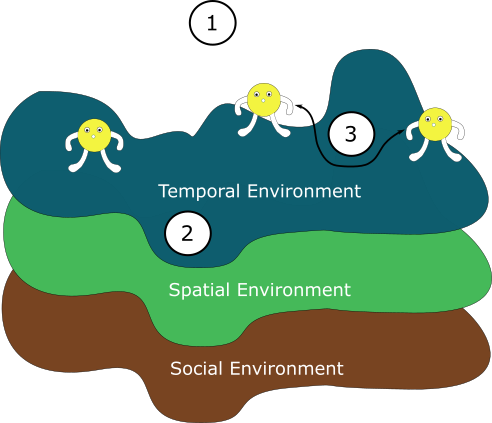
\includegraphics[width=1.2\textwidth]{figures/temporalRepresentation.png}
    \end{figure}
\end{column}
\begin{column}{.60\linewidth}
\begin{enumerate}
    \item The \textbf{Agent-Group-Role-Environment-Time (AGRET)} model : a MAS design methodology that articulates the spatial, organizational and temporal dimension
    \medbreak
    \item The \textbf{temporal environment} : an interaction environment for sharing, storing and perceiving temporal information
    \medbreak
    \item The \textbf{Influence-Reaction Model For Simulation (IRM4S)}: an interaction model that links the agents and the temporal environment
\end{enumerate}
\end{column}
\end{columns}
    
\note{
Pour mettre en place ce nouveau support au sein du système existant, nous proposons un ensemble de solutions axé sur trois points:
\begin{enumerate}
    \item une méthodologie de conception permettant d’articuler les 3 dimensions spatiale, organisationnelle et temporelle. Nous appelons cette approche AGRET.
    \item Un milieu d’interaction qui permet le stockage et l’accès aux informations temporelles. Nous appelons ce milieu environnement temporel.
    \item un modèle d’interaction qui permet le lien entre les agents et le milieu d’interaction. Nous utilisons un modèle existant : IRM4S, que nous appliquons à l'environnement temporel.
\end{enumerate}
Je vais donc présenter brièvement chaque solution.
}
    
\end{frame}

\begin{frame}{1. Agent-Group-Role-Environment-Time (AGRET)}
\par \textbf{Objective}: naturally and equally take the spatial, temporal and organizational dimensions into account

\par \textbf{Proposition}: The AGRET model consists of an extension and an enrichment of one of the most well-known and widely used organizational approaches in MAS: AGR and its extension AGRE.
\begin{itemize}
    \item AGR takes into account only the organizational dimension
    \item AGRE adds the \say{located in space} aspect to AGR: takes into account both the organisational and the spatial dimension equally
    \item AGRET adds the \say{located in time} aspect to AGRE: takes into account the organisational, spatial and temporal dimensions in the same way

\end{itemize}
    
\note{
Agent-Groupe-Rôle-Environnement-Temps est une approche qui prend en compte naturellement et au même titre les dimensions spatiale, temporelle et organisationnelle.
Elle se base sur une des approches organisationnelles les plus connus et la plus communément utilisée dans les SMA : AGR et de sa variante AGRE, que nous étendons et enrichissons. Il rajoute l'aspect situé dans le temps aux deux aspects situés dans l'espace et dans la dimension sociale d'\gls{agre}. \gls{agre} est elle-même une extension du modèle générique d'organisation \gls{agr}. Il ajoute la prise en compte de l'environnement spatial au modèle \gls{agr} qui ne considère que les organisations.
}
\end{frame}

\begin{frame}{1. Agent-Group-Role-Environment-Time (AGRET)}
\begin{figure}
	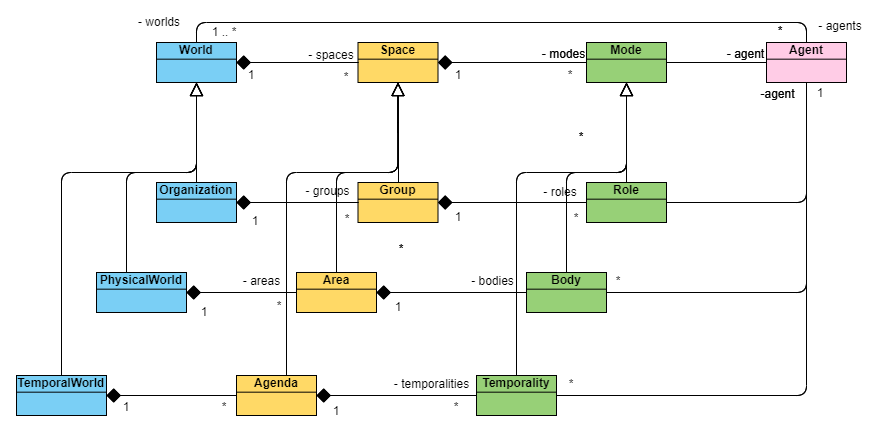
\includegraphics[width=\textwidth]{figures/agret.PNG}
\end{figure}
\note{
Voici le diagramme UML correspondant à notre modèle AGRET. Je vais vous montrer petit à petit l'évolution de ce modèle jusqu'à ce que nous proposons AGRET.
}
\end{frame}

\begin{frame}{1. Agent-Group-Role-Environment-Time (AGRET)}{AGR}
\begin{figure}
	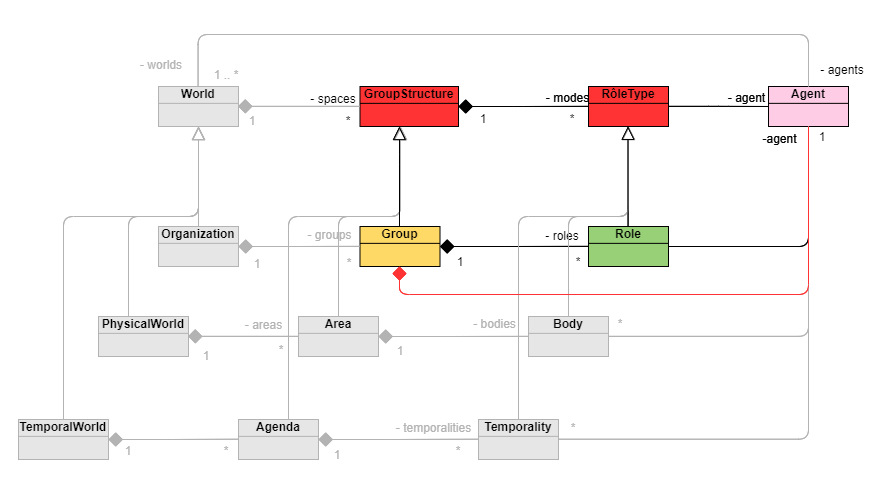
\includegraphics[width=\textwidth]{figures/agr.png}
\end{figure}

\note{
\par Le diagramme UML correspondant à AGR est celui qui n'est pas grisé. Le lien en rouge est propre à AGR. L’organisation d’AGR s'articule autour de trois notions : Agent, Groupe, Rôle
\begin{enumerate}
    \item Un agent est une entité active et communicante. 
    \item Un groupe est un ensemble d'agents partageant des caractéristiques communes. 
    \item Un rôle est la représentation abstraite d'une position fonctionnelle d'un agent dans un groupe.
\end{enumerate}
Un agent joue un rôle dans un ou plusieurs groupes, peut tenir plusieurs rôles et peut être membre de plusieurs groupes.
}
\end{frame}

\begin{frame}{1. Agent-Group-Role-Environment-Time (AGRET)}{AGRE}
\begin{figure}
	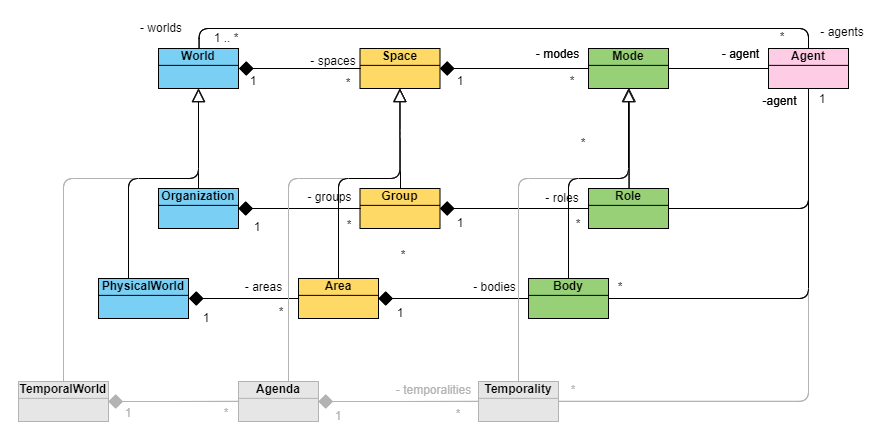
\includegraphics[width=\textwidth]{figures/agre.png}
\end{figure}

\note{
AGRE vient alors compléter l’aspect situé corporel à l’aspect situé social d'AGR. AGRE défini, en plus du concept d'agent, trois concepts généraux qui se déclinent en concepts spécifiques selon le type d'environnement (organisationnel ou spatial) :
\begin{enumerate}
    \item Un espace est un domaine dans lesquels les agents sont situés.
    \item Un mode est la manifestation d'un agent dans un domaine spécifique, son mode d'existence et son apparence dans un espace. Un mode décrit la position de l'agent et la manière dont il perçoit et agit dans un space.
    \item Un monde est une collection de spaces de même type. 
\end{enumerate}
AGRE définit deux types de mondes : les organisations qui représentent l'environnement social et qui sont composées de groupes et le monde physique qui représente l'environnement physique et qui est composé de zones. Les agents sont alors situés dans les spaces et peuvent y agir à travers les modes. Un mode dans une zone est appelé corps (body) tandis qu'un mode dans un groupe est appelé rôle (role).
Dans leur article  Ferber et al. considèrent uniquement deux types de monde. Néanmoins, ils évoquent la possibilité d'existence d'autres types de monde et d'autres types d'espace qu'ils ne décrivent pas dans leur article. 

}
\end{frame}

\begin{frame}{1. Agent-Group-Role-Environment-Time (AGRET)}
\begin{figure}
	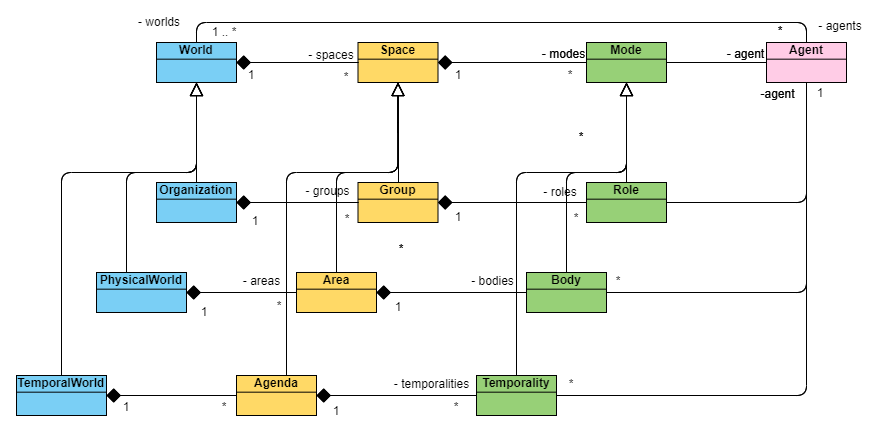
\includegraphics[width=\textwidth]{figures/agret.PNG}
\end{figure}
\medbreak
\par \textbf{Originality}: Consideration of the temporal dimension as a medium of interaction, \alert{the temporal environment}
    
\note{
Dans AGRET, nous reprenons les principes de base d'AGRE et nous ajoutons la dimension temps. Nous définissons alors un nouveau type d'espace qui est de type temporel et que nous appelons agenda. Comme dans AGR et AGRE, les agents sont situés dans les espaces et peuvent y agir à travers les modes. Si un mode dans une zone est appelé corps (body), un mode dans un groupe est appelé rôle (role), nous appelons un mode dans un agenda une  temporalité (temporality). Un nouveau type de monde vient également s'ajouter à ces deux types de monde déjà existants dans AGRE: le monde temporel (temporal world).
La figure montre un diagramme UML simplifié qui représente les relations entre mondes, espaces, zones, groupes, agendas, modes, corps, rôles et temporalités.

\par Une des originalités de notre proposition, comparée à d'autres approches de gestion du temps est la représentation du temps simulé comme un milieu d'interaction. Nous avons appelé ce milieu d'interaction environnement temporel. Cet environnement temporel vient en complément à l'ordonnanceur de la simulation. 
}
\end{frame}

\begin{frame}{2. The Temporal Environment}{An interaction medium}
\par \textbf{Observation}: Most of the time, the spatial and organizational dimensions are modeled as environments
\medbreak
\par \textbf{Proposition} : modelling the temporal dimension as an environment called the \textbf{temporal environment} 
\medbreak
\begin{block}{Remarks}
The temporal environment does not replace the scheduler but complements its role
\begin{itemize}
    \item It comes between the scheduler and the agent
    \item It breaks the direct link between the agent and the scheduler
\end{itemize}
\vspace{.3cm}
\par The the temporal dimension management is done on two levels
\begin{itemize}
    \item \textbf{Temporal environment}: representation of temporal dynamics, exchange
    \item \textbf{Scheduler}: management of the simulation activation cycle
\end{itemize}
\end{block}
    
\note{
En partant du constat que les dimensions spatiale et organisationnelle sont modélisé, la plupart du temps, sous forme d’environnements, nous proposons une modélisation du temps sous forme d’environnement. Nous appelons cet environnement : l’environnement temporel. Il s’agit d’un espace dont la métrique est le temps.
Nous tenons tout de même à noter que l’environnement temporel ne remplace pas l’ordonnanceur de la simulation, il  vient compléter son rôle. L’environnement temporel vient s’interfacer entre l’agent et l’ordonnanceur cassant le lien direct entre ces derniers.
La gestion de la dimension temporelle se fait alors sur deux niveaux:
\par L’environnement temporel gère la représentation de la dynamique d’activation temporelle des agents ainsi que les échanges d’informations sur cette dimension temporelle
\par L’ordonnanceur gère le cycle d’activation de la simulation
Nous reviendrons plus en détails sur ces deux niveaux lorsque nous aborderons l’aspect modèle d’interaction.
}
\end{frame}

\begin{frame}{2. The Temporal Environment}{An Interaction Medium}
\par \textbf{Structure and mechanics} based on the Temporality Model
\vspace{.5cm}
\begin{block}{Temporality Model}
\begin{itemize}
    \item  A time scheduling approach (used only by the scheduler)
    \item Research work of our CAS working group (Dr. Payet)
\end{itemize}
\end{block}
\vspace{.5 cm}
\par \textbf{Proposition}: redesign the temporality model in order to reuse its basic principles in the structuring and the implementation of the temporal environment mechanics
\medbreak
\Centering{
\par Use of the temporality model in the level of:\\
the scheduler (Dr Payet) \alert{$\ne$} the temporal environment (My thesis)}


\note{
Un environnement possède une structure, un ensemble de mécaniques et une dynamique qui lui sont propre. La structure et les mécaniques propres à l’environnement temporel se basent sur les principes du modèle à temporalité. Le modèle à temporalité est une approche qui à l’origine était utilisé uniquement au niveau de l’ordonnancement de la simulation, au même titre que l’approche à pas de temps constant, l’approche événementielle ou l’approche hybride. Elle fait partie des contributions de notre équipe de recherche, plus précisément des travaux de Mr Payet. Dans cette thèse, je procède à une refonte du modèle pour une réutilisation de ses principes de base dans la structuration et la mise en place des mécaniques de l’environnement temporel. Il est donc très important de bien distinguer l’utilisation de l’approche de type modèle à temporalité pour l’ordonnancement de la simulation et de sa réutilisation pour la structuration et la mise en place des mécaniques de l’environnement temporel. Cette deuxième fait partie des contributions de cette thèse.
}
    
\end{frame}

\begin{frame}{2. The Temporal Environment}{An Interaction Medium}
\textbf{Use of the temporality model at the level of the \alert{scheduler}}
\begin{itemize}
    \item A particular type of time scheduling approach
    \item An expressive approach: allows the agent to describe his own temporal dynamics (sharing of temporal information)
    \item Integrates a support that allow representing this dynamic in the form of:
\end{itemize}

\begin{figure}
	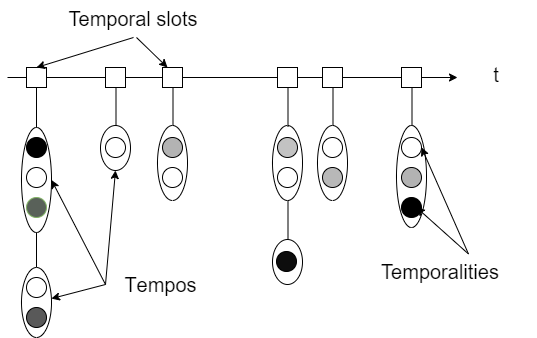
\includegraphics[width=.5\textwidth]{figures/temporalityModel.png}
\end{figure} 
\par \textbf{Limit}: allows neither the storage of temporal information nor its access
\note{
\footnotesize{Comparée aux autres approches d'ordonnancement du temps, nous pensons que le modèle à temporalité est intéressante pour la structuration de l'environnement temporelle car
\par C'est une approche expressive: ie, elle permet aux agents de définir eux-mêmes et de partager leur dynamique d'activation temporelle.
\par De plus , elle intègre également un support permettant de représenter cette dynamique sous forme de temporalités, tempos, d'axe temporel et de slots temporels. Dans le modèle à temporalité, l'agent indique à l’ordonnanceur de la simulation à quelle moment il souhaite être réveillé ou activé en définissant une structure de donnée appelée temporalité. Le traitement interne des temporalités par l'ordonnanceur fait intervenir deux structures de données: le slot temporel et le tempo. L’ordonnanceur fait progresser  le temps simulé  en l’emmenant successivement sur chacune des positions signalées par un slot temporel.
\par Nous avons donc là une approche qui permet le partage et la structuration des informations temporelles. Cependant, cette mécanique ne permet ni le stockage des informations ni leur perception.
\par En effet, les temporalités passées sont supprimés car elles n'interviennent plus dans le cycle d'activation de la simulation et l'ordonnanceur calcule les prochaines dates de déclenchement des temporalités futures avant chaque avancement du temps. Il s'agit d'un comportement tout à fait normal compte tenu de l'objectif qui est l'ordonnancement du temps.
\par Cependant, le stockage et la perception des informations sont indispensables au niveau de l'environnement temporel. Nous procédons alors à une refonte du modèle en intégrant notamment ces possibilités.

}
}
\end{frame}

\begin{frame}{2. The Temporal Environment}{An Interaction Medium}
\textbf{Use of the (modified version of) temporality model at the level of the \alert{temporal Environment}}
\begin{itemize}
    \item Structure : time axis, tempo, temporal slot, etc.
    \item Environmental Mechanics
\end{itemize}
%\vspace{.5cm}
\begin{table}[]
\resizebox{\textwidth}{!}{%
\begin{tabular}{ll}
\hline
\rowcolor[HTML]{34495E} 
{\color[HTML]{FFFFFF} Scheduler}                     & {\color[HTML]{FFFFFF} Temporal Environment}                                                                                                                                                                                     \\ \hline
\multicolumn{1}{|c|}{-}                              & \multicolumn{1}{l|}{\alert{Temporality}: representation of the agent in the temporal environment}                                                                                                                                      \\ \hline
\multicolumn{1}{|l|}{\alert{Temporality} $t=\{id,d,f,p,v\}$} & \multicolumn{1}{l|}{\begin{tabular}[c]{@{}l@{}}\\[.2cm]\alert{Temporal location} $l=\{\underbrace{id,d,f,p,v}_{Mandatory\ parameters} ,\underbrace{...}_{optional\  parameters}\}$\\[1cm] * Optional parameters. Ex: queue, cost, criticality, priority, accessibility, etc.\end{tabular}} \\ \hline
\multicolumn{1}{|l|}{Temporal Slot}                  & \multicolumn{1}{l|}{Temporal Slot}                                                                                                                                                                                              \\ \hline
\multicolumn{1}{|l|}{Tempo}                          & \multicolumn{1}{l|}{Tempo}                                                                                                                                                                                                      \\ \hline
\multicolumn{1}{|l|}{\begin{tabular}[c]{@{}l@{}}No storage:\\ - The next activation dates of future temporalities \\ are calculated before each advance of time\\ - Temporalities are removed after activation\end{tabular}}                          &
\multicolumn{1}{l|}{\begin{tabular}[c]{@{}l@{}}- Storage of past, present and future information\\ - Storage Time Window $\Delta_s=[\delta_{smin}, \delta_{smax}]$\end{tabular}} \\ \hline
\multicolumn{1}{|l|}{
No possibility of collecting information}                                                                                                                                                                              & 
\multicolumn{1}{l|}{Ability to perceive past, present and future information}                                                                                                   \\ \hline
\end{tabular}
}
\caption{Use of the temporality model at the scheduler level and at the level of the temporal environment: comparison and equivalence }
\end{table}


    
\note{\footnotesize{Ce tableau présente les correspondances entre les principes de bases de l’approche de type modèle à temporalité lorsqu’ils sont utilisé pour l’ordonnancement de la simulation et lorsque nous ré-adaptons pour une utilisation dans le cadre de l’environnement temporel.
\par Dans l’environnement temporel, une temporalité est la représentation de l'agent dans l'environnement temporel,  au même titre que le corps de l'agent dans l'environnement spatial ou le rôle dans l'environnement social. Cette notion est propre à l'environnement temporel. Il n'a donc pas d'équivalent au niveau de l'ordonnanceur. Le corps possède une localisation spatiale dans l'environnement physique. Son déplacement se traduit par la modification de sa localisation spatiale. De la même manière, une temporalité possède une localisation temporelle dans l'environnement temporel. Son déplacement se traduit par la modification de sa localisation temporelle. C'est cette notion de localisation temporelle dans l'environnement temporel qui est équivalente à la notion de temporalité dans le modèle à temporalité au niveau de l'ordonnanceur. 
\par Cette localisation temporelle est définie par un ensemble de paramètres obligatoires et des paramètres optionnels qui peuvent être ajoutés en fonction des besoins du modèle. Par exemple, dans notre cadre applicatif, nous ajoutons l'estimation de la longueur de la file d'attente, le cout correspondant, etc. comme paramètre optionnel.
\par Les notions de tempo et de slot temporels quant à eux restent les mêmes.
\par Nous mettons également en place un le stockage et la perception des information positionnées sur le passé, sur le présent et sur le futur. 
\par Par ailleurs, la pertinence de ces informations varie en fonction du temps, du modèle et du type d'information. Une information passée peut avoir une durée de vie au-delà de laquelle elle devient obsolète. De même, au-delà d'une certaine limite dans le temps, une information future n'est pas forcément pertinente. Nous mettons en place un horizon temporel de stockage  dont les valeurs des bornes sont définies arbitrairement par l'utilisateur ou le concepteur du modèle.
\par
}
}
\end{frame}

\begin{frame}{2. The Temporal Environment}{An Interaction Medium}
\alert{Remarks:}
\begin{itemize}
    \item The readaptation of the basic principles of the temporal model for use in the temporal environment is \textbf{completely independent} of the scheduling approach used in the scheduler of the simulation
    \item We can set up a temporal environment that can be coupled with a scheduler that uses another type of approach: time-stepped, event-driven, etc.

\end{itemize}
\note{
Il est important de noter que la ré-adaptation des principes de bases du modèle à temporalité pour une utilisation au niveau de l’environnement temporel est tout à fait indépendante de l’approche d’ordonnancement utilisé au niveau de l’ordonnanceur de la simulation. Ainsi, il est tout à fait possible de mettre en place un environnement temporel que l’on couple avec un ordonnanceur qui utilise un autre type d’approche : à pas de temps constant, événementielle, etc.

}
\end{frame}

\begin{frame}{3. IRM4S}{An Interaction Model}
2 types of interaction models:
\begin{itemize}
    \item Action/Reaction: \footnote{$Behaviour_a$ describes the activation cycle of the agent $a$ : perception, deliberation, action or influence }$Behaviour_a :\footnote{$\Sigma$ is the environment state}\Sigma \mapsto \Sigma$
    \item Influence/Reaction: $Behaviour_a: \footnote{$\Gamma$ is an influence : does not directly change the state of the environment. It represents an agent's desire to see it changed in some way}\Gamma \mapsto \Gamma$
\begin{itemize}
    \item Compliance with the environmental integrity constraint
    \item Respect for the autonomy of the agents
    \item Reduction of the agent-action-environment coupling: the simulation is less sensitive to the way it is implemented
    \item Clearly distinguishes between agent and environment
\end{itemize}
\end{itemize}
\textbf{IRM4S}: $ Behaviour_a: \Sigma \times \Gamma \mapsto \Gamma$
\begin{itemize}
    \item Approach adapted to multi-agent simulation
    \item Takes into account an agent's local and subjective perception of his environment
\end{itemize}
\note{

Maintenant, je vais vous introduire le modèle d’interaction qui permet de définir le lien entre l’agent et l’environnement. Ce lien se traduit par le fait que l’agent perçoit son environnement et agit sur ce dernier. 
\par Nous choisissons d'utiliser IRM4S qui 
simplification” et une clarification du modèle influence/réactio dans le cadre de la simulation multi-agent. Comme dans toute approche de type i/r, le cycle comportemental de l'agent, traduit par la fonction behaviour, aboutit à la production d'influences. Cependant, dans le modèle i/r, les agents perçoivent ce qui les influence, mais ne sont pas influencés par l'état de l'environnement.
\par Contrairement à cela, IRM4S prend en compte la perception locale et subjective de son environnement par un agent. Nous utilisons IRM4S dans le cadre de la mise en place de l’environnement temporel.

%Il existe deux types de modèles d’interactions communément utilisé dans les SMA. Nous choisissons de nous pencher sur un modèle i/r car il respecte la contrainte d’intégrité environnementale et la propriété d’autonomie des agents du système. Il permet donc de réduire le couplage entre agent-action-environnement. Ainsi, le modèle est moins sensible à la manière dont il est implémenté. 
%\par Le cycle comportemental classique d’un agent se résume en trois phases: perception, délibération, action ou influence. Ce cycle est traduit par une fonction $Behaviour_a$. Dans l'approche a/r, il aboutit à une transformation directe de l’environnement. Contrairement à cela, dans le modèle i/r, il aboutit à une influence. L'influence diffère de l’action dans le sens où elle ne modifie pas directement l'environnement. Elle représente le souhait d'un agent de le voir modifié d'une certaine façon. Ce modèle distingue alors bien tout ce qui relève de l’agent de tout ce qui relève de l’environnement. En d'autres termes, un agent ne peut que décider de l'action suivante à faire. C'est à son environnement de déterminer les conséquences de cette dernière. Par exemple : un agent décide de faire déplacer un objet de l’environnement, mais c'est son environnement (son corps et son environnement extérieur) qui exécute le déplacement.
%\par Ferber et al. proposent une “simplification” et une clarification du modèle i/r dans le cadre de la simulation multi-agent. Le modèle s'appelle IRM4S. Il s'agit d'une approche adaptée dans un contexte de simulation multi-agent.
%\par Comme dans toute approche de type i/r, dans IRM4S le cycle comportemental de l'agent aboutit à la production d'influences. Cependant, dans le modèle i/r, les agents perçoivent ce qui les influence, mais ne sont pas influencés par l'état de l'environnement. \par Contrairement à cela, IRM4S prend en compte la perception locale et subjective de son environnement par un agent. Nous utilisons IRM4S dans le cadre de la mise en place de l’environnement temporel.
}

\end{frame}

\begin{frame}{3. IRM4S}{An Interaction Model}
\pa The introduction of the temporal environment induces consequences on 2 levels:
\begin{enumerate}
    \item The agent activation cycle
    \item The simulation activation cycle
\end{enumerate}

\begin{block}{The agent activation cycle}
\par Perception time window $\Delta_{pt}=[\delta_{ptmin},\delta_{ptmax}]$ (the agent has a limited perception of its environment)
\vspace{.5cm}
\begin{equation*}
    Perception:\Sigma \times \Gamma \times  \footnote{Temporal, spatial, social perception window}\alert{\Delta_p} \mapsto P
\end{equation*}

\end{block}

\note{

\par L'introduction de l'environnement temporel induit des conséquences au niveau du modèle d'intéraction sur 2 niveaux:
\begin{enumerate}
    \item Au niveau du cycle d'activation des agents
    \item Au niveau du cycle d'activation de la simulation
\end{enumerate}
\par Au niveau du cycle d'activation des agents: pour chaque agent ou chaque type d'agent, nous définissons une fenêtre temporelle ou horizon temporel de perception noté $\Delta_p=[\delta_{pmin},\delta_{pmax}]$ . Cette horizon temporelle contraint la perception et traduit une propriété de l'agent : celle d'avoir une perception limitée de son environnement temporel. Il s'agit de l'équivalent temporel du champ de vision dans l'environnement spatial. 
La perception est donc donnée par la fonction suivante
où $\Sigma$ est l'état de l'environnement, $\Gamma$ est un ensemble d'influences, $\Delta_p$ est la fenêtre temporelle de perception et $P$ est un ensemble de percepts. 
\par Nous pouvons notamment noter la prise en compte, de manière explicite, de les horizons de perception dans la formalisation de la perception.
}
\end{frame}

\begin{frame}{3. IRM4S}{An Interaction Model}
\begin{block}{The simulation activation cycle}

\par \alert{Classical} simulation activation cycle:
\begin{enumerate}
    \item \textbf{environments activation}: These environments have states that evolve over time according to their own inertial laws, and the influences exerted by the agents : \textbf{time constrained environment}
    \item \textbf{agents activation}
\end{enumerate}
\vspace{.5cm}
\par \alert{New} simulation activation cycle:
\begin{enumerate}
    \item \textbf{time-constrained environments activation} phase over the time interval $]t-dt; t]$. Example : spatial environment, social environment
    \item \textbf{agents activation} phase on the current time time $t$;
    \item \textbf{non-constrained environments} activation phase on the consideration that $t$ is over. Example : temporal environment
    \begin{itemize}
        \item The temporal environment state determines the temporal dynamics
        \item The state of the temporal environment evolves out of time
    \end{itemize}
\end{enumerate}

\end{block}

\note{
\par Au niveau du cycle d'activation de la simulation: Dans la plupart des simulateurs, la phase d'activation de l'environnement se déroule en début du cycle d'activité de la simulation. Cela est dû au fait que la plupart des environnements a besoin de calculer son nouvel état en début d'un cycle (instant $t$), avant l'activation des agents. Ces calculs doivent  s'établir sur l'intervalle de temps qui s'est écoulé depuis la dernière activation. Ces environnements ont des états qui évoluent dans le temps en fonction des lois inertielles qui leur sont propres, et des influences qu'exercent les agents. Ce sont donc, en quelque sorte, des environnements contraints par le temps.
\par Dans notre contexte, la mise en place d'un nouveau type d'environnement qui est l'environnement temporel vient chambouler le fonctionnement de ce cycle classique d'ordonnancement de la simulation. Par définition, l'état de l'environnement temporel détermine la dynamique d'écoulement du temps. Par conséquent, son état évolue hors du temps. \textbf{L'environnement temporel n'est pas un environnement contraint par le temps}. 
Ainsi, aux deux phases du cycle d'activation classique de la simulation s'ajoute alors une troisième phase : la phase d'activation des environnements non contraints par le temps sur la considération que $t$ vient d'être passé.


}
\end{frame}

\begin{frame}{Summary}
\begin{figure}
	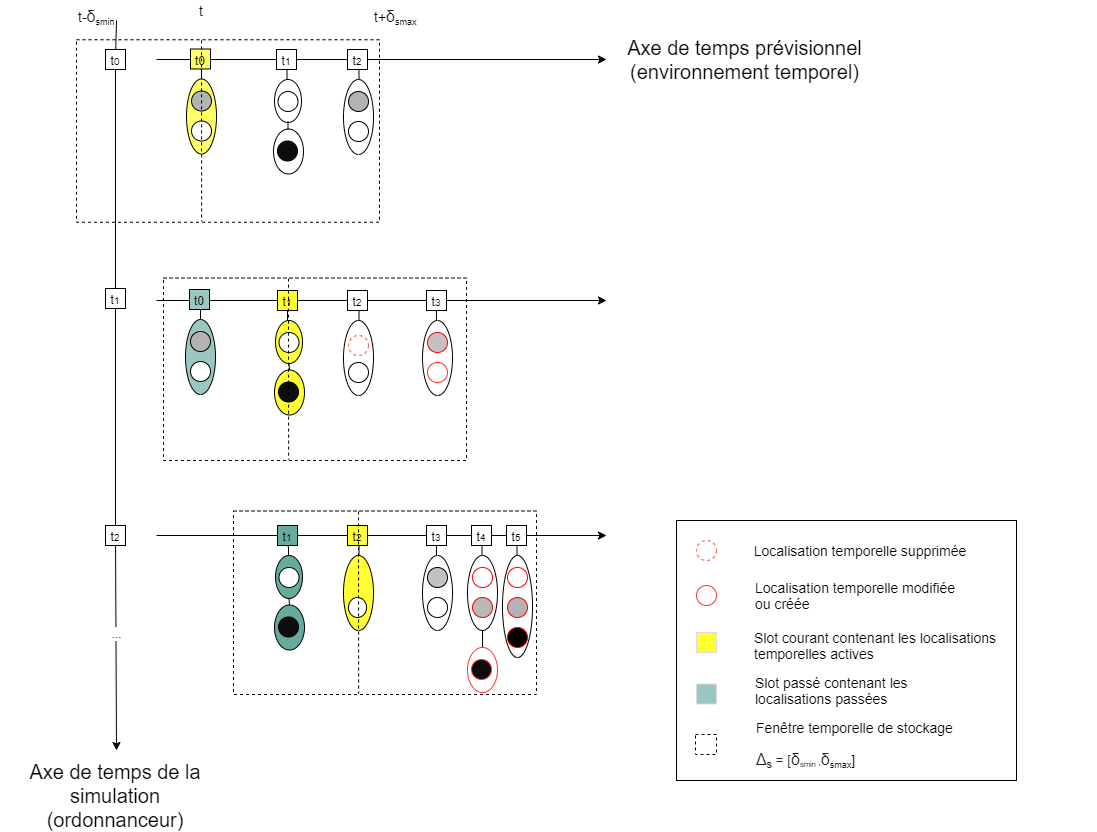
\includegraphics[width=.7\textwidth]{figures/EnvironnementTemporel.png}
	\caption{State of the temporal environment at each advance in time}
	\end{figure}

\note{Pour résumer, le schéma suivant illustre l’état (statique) de l’environnement temporel à chaque avancement du temps simulé: Cet état est donné par l’ensemble des localisations temporelles définies par tous les agents du système.
Nous distinguons notamment deux axes : 
l’axe de temps de la simulation qui correspond à l’horloge globale de la simulation et qui est gérée par l’ordonnanceur,
 l’axe de temps prévisionnel qui est l’axe de temps stocké au niveau de l’environnement temporel et qui traduit la dynamique prévisionnelle d’activation des agents. Cet axe de temps prévisionnel contient des localisations temporelles passées, présentes et futures.
}
\end{frame}

\begin{frame}{Summary}
	\begin{figure}
	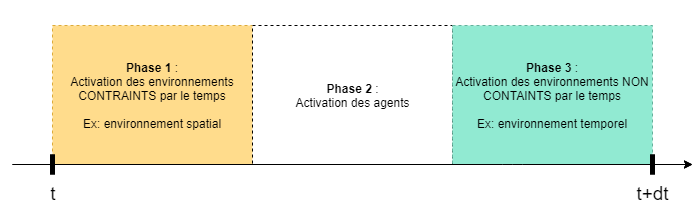
\includegraphics[width=\textwidth]{figures/Cycle_activite.png}
	\caption{New simulation activation cycle}
	\end{figure}
	
\note{
 \par L'introduction de l'environnement temporel conduit à l'ajout d'une 3ème phase au cycle d'activation de la simulation : la phase d'activation des environnements non-contraints par le temps.

}
\end{frame}

\begin{frame}{Implementation}
    \begin{figure}
	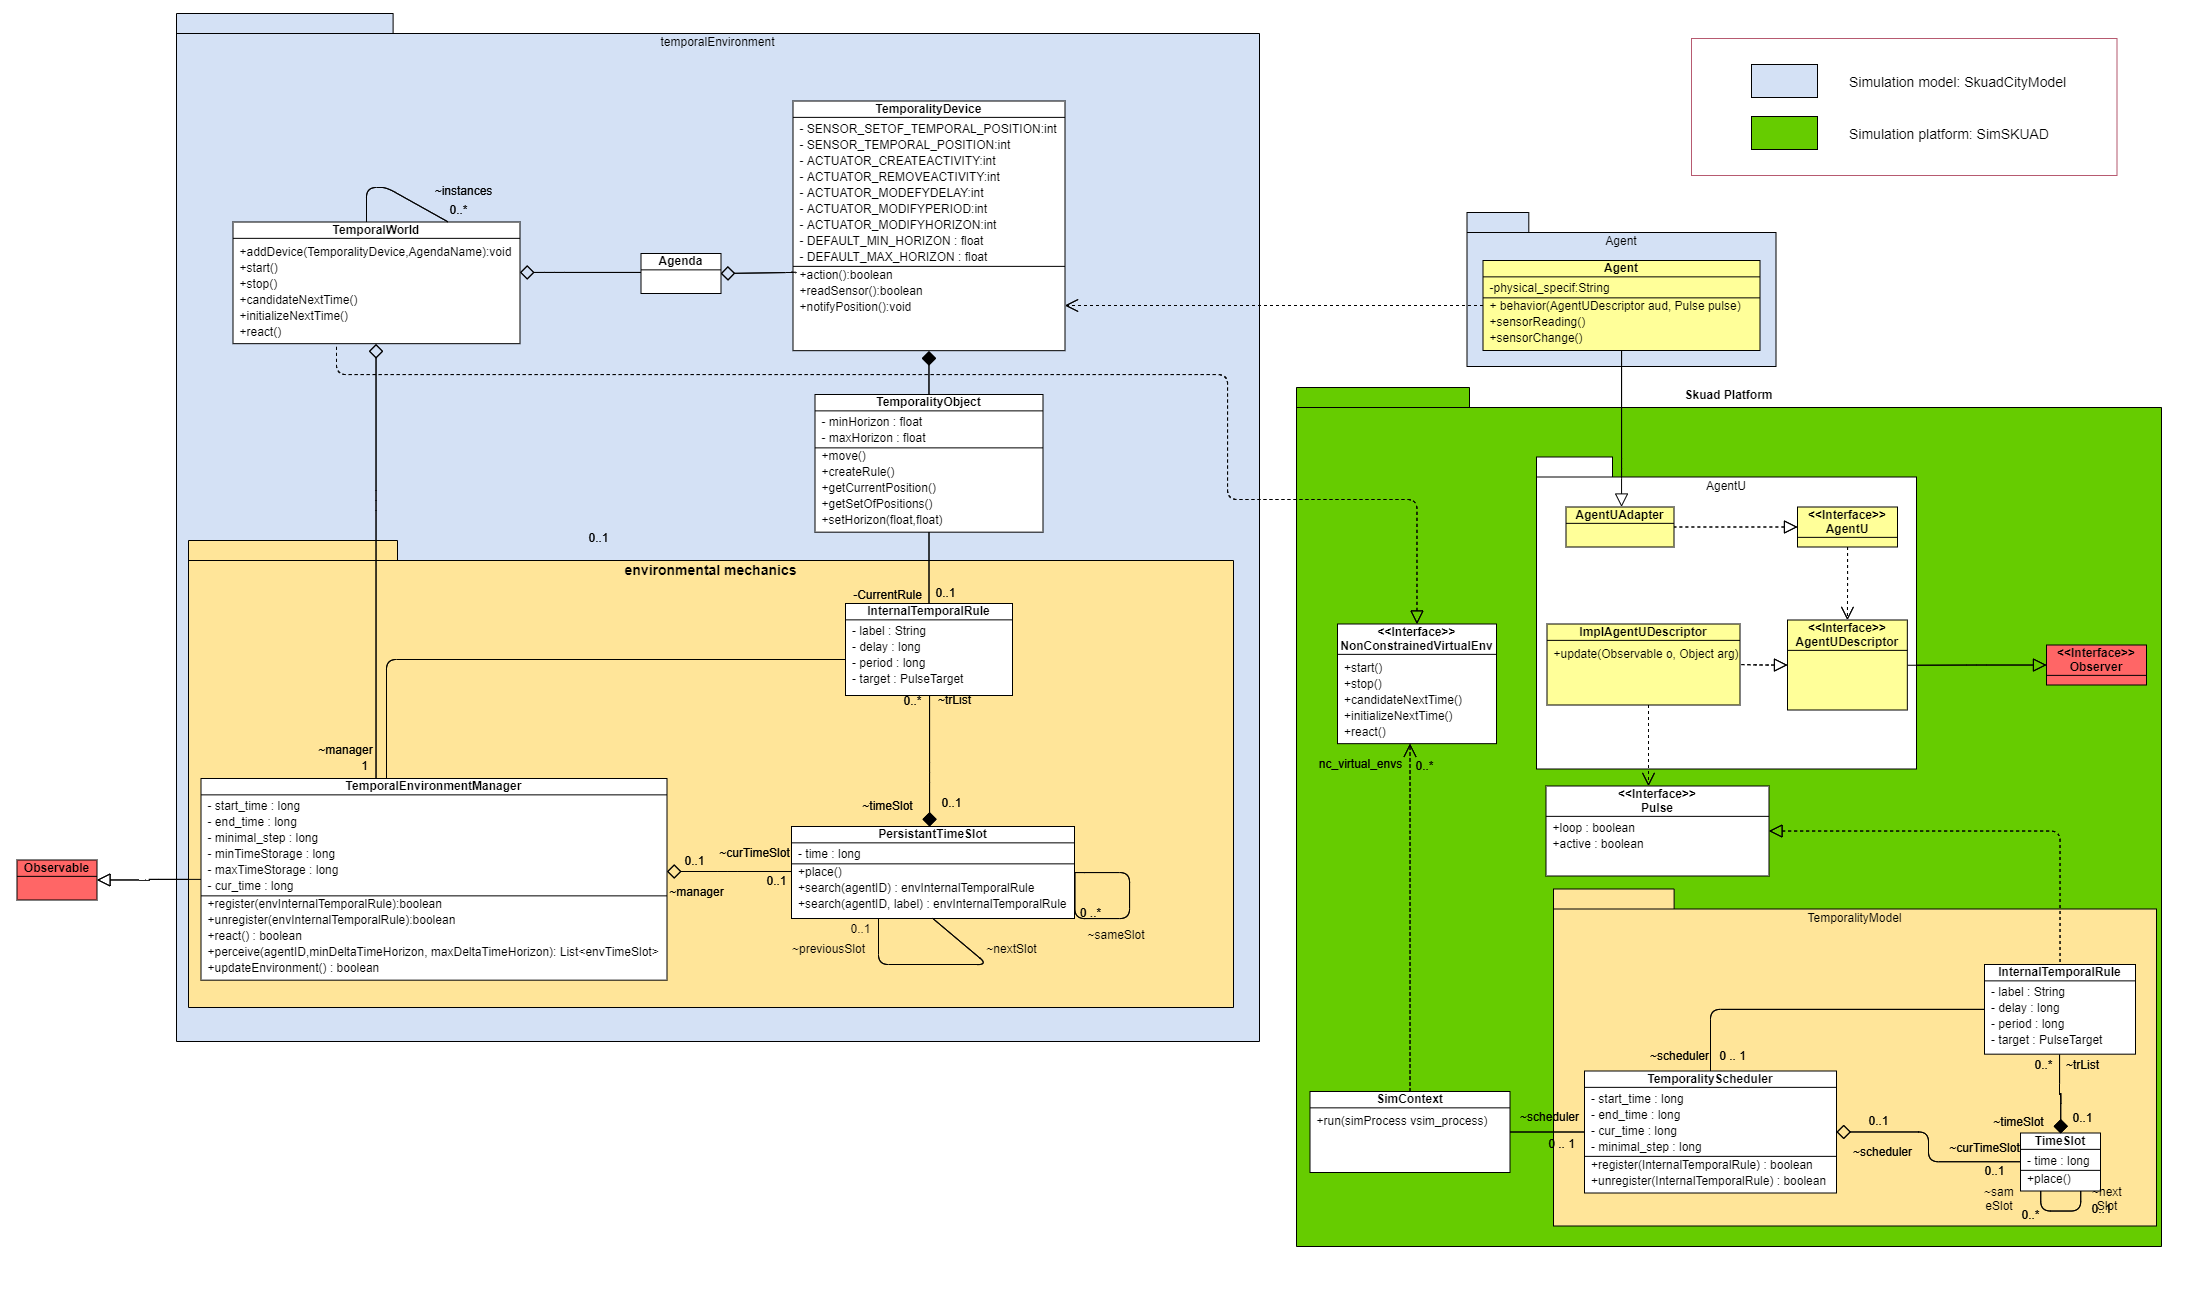
\includegraphics[width=\textwidth]{figures/temporalEnvironmentImpl.png}
	\end{figure}
\note{
Dans SkuadCitymodel, l’implémentation de notre première contribution s’effectue sur deux niveaux:
\begin{itemize}
    \item au niveau du modèle de simulation : implémentation de l’environnement temporel. 
    \item au niveau de la plateforme de simulation : mise à jour du mécanisme de gestion du cycle d’activation de la simulation. La mise en oeuvre au niveau de la plateforme de simulation, plus précisément au niveau de l’ordonnanceur consiste en la modification du cycle d’activation de la simulation afin de respecter les 3 phases que j’ai présenté précédemment: nous avons notamment mis en place la mise à jour des environnements non-contraints par le temps en début de cycle.
\end{itemize}
L’implémentation de l’environnement temporel au niveau du modèle de simulation se divise en deux parties:
\begin{itemize}
    \item la mise en oeuvre de la structure de l’environnement sur la base du modèle AGRET
    \item les mécaniques environnementaux
\end{itemize} 

}
\end{frame}

\begin{frame}{Implementation}{Structure}
2 types of environment in SimSKUAD:
\begin{enumerate}
    \item Physical
    \begin{itemize}
        \item the link between the agent and its representation in the environment is made by cabling using a physical slot
        \item Agent representation: body + device (integrates sensors and actuators)
        \item Ex : spatial environment, \textbf{temporal environment}
    \end{itemize}
    \item Social
    \begin{itemize}
        \item the link between the agent and the environment is made by cabling using a social slot
        \item Agent representation: avatar
        \item Ex : social environment
    \end{itemize}
\end{enumerate}
\vspace{.5cm}
\centering{\alert{The temporal environment} is implemented in the form of a \alert{physical environment.}}

\note{Dans tout modèle de simulation développé sur SimSKUAD, nous distinguons deux types d’environnements : l’environnement physique et l’environnement social. Techniquement parlant, l’environnement est dit physique lorsque le lien entre l’agent et sa représentation dans l’environnement se fait par cablâge via un slot physique. Cela lui permet de disposer d’une représentation physique et d’une entité que nous appelons device. Le device est un objet de l’environnement, des dispositifs matériels intégrant des capteurs et des actionneurs que les agents utilisent pour interagir avec un environnement physique. L’environnement est dit social lorsque le lien entre l’agent et l’environnement se fait par cablâge via un slot social. Cela lui permet de disposer d’une représentation dans l’environnement social appelée avatar. Pour faire simple, un avatar est un objet qui fournit des outils permettant d'opérer des modifications sur la dimension sociale (communiquer par message par exemple). L’environnement temporel est mise en oeuvre sous la forme d’un environnement physique. Cela permet à l’agent de disposer d’une temporalité qui est composé d'un corps et d’une device temporel qui intègre les capteurs et les actionneurs nécessaires à la manipulation de l’environnement temporel par les agents. Nous avons également sur le schéma l’espace qui est l’agenda et le monde temporel.}
    
\end{frame}

\begin{frame}{Implementation}{Environmental mechanics}
    \begin{figure}
	\includegraphics[width=\textwidth]{figures/temporalEnvironmentImpl.png}
	\end{figure}
\note{
Les mécaniques environnementaux qui reprennent les principes de base du modèle à temporalité. Comme vous pouvez le constater sur le schéma nous faisons le parallèle entre les mécaniques du modèle à temporalité utilisé au niveau de l’ordonnanceur et ceux ré-utilisés au niveau de l’environnement temporel. Nous pouvons notamment constater des différences par exemple au niveau de l’environnement temporel la possibilité de naviguer dans les 2 sens (vers le passé et vers le futur), la gestion du stockage, de la mise à jour, la réaction et la perception de l’environnement temporel.
\par Au niveau du modèle de simulation, notre implémentation de l’environnement temporel est assez générique pour être ré-utilisable facilement dans d’autres modèles de simulation tournant sur SimSKUAD.
\par De même les modifications effectuées au niveau de la plateforme de simulation ne devrait avoir aucune incidence sur les modèles de simulation déjà existantes tournant sur SimSKUAD.
}
    
\end{frame}
%\subsection{Anticipatory Reasoning in ABMs: Benefits of the AGRET Model (Chapter 4)}
%\begin{frame}{Anticipatory reasoning}
\textbf{Objectives}:
\begin{itemize}
    \item Assess or reassess the feasibility of carrying out an activity
    \item Select the most relevant activity to be carried out
    \item Enrich and bring more precision to the agent's activity planning
\end{itemize}
\vspace{.3cm}
\par \textbf{Observation}: In most MAS anticipation approaches, the agents
\begin{itemize}
    \item can't get any information about what the other agents are planning to do
    \item are forced to try to predict what is going to happen in the future by performing microsimulations internally
\end{itemize}
\vspace{.3cm}
\par \textbf{Proposition}: Exploit the AGRET model
\begin{itemize}
    \item offers visibility on the future dimension of time
    \item take into account the three positions of time: past, present, and future. \alert{The consideration of the future position of time is original}
\end{itemize}

\note{
Maintenant que le support permettant l’échange d’informations sur les 3 dimensions : espace, temps et organisation est posé, je vais vous montrer comment nous l'exploitons afin d'enrichir les informations prises en compte dans le raisonnement anticipatif de l'agent. Les objectifs sont :
\begin{itemize}
    \item évaluer ou réévaluer la possibilité d'exécution d'une activité;
    \item choisir l'activité la plus pertinente à exécuter;
    \item enrichir et apporter plus de précision au planning d'activités de l'agent.
\end{itemize}
\par Pour se faire, nous exploitons AGRET et plus particulièrement la visibilité qu'il offre sur la position future du temps. Ces informations futures concernent les activités que les agents projettent d'effectuer. En effet, dans la plupart des approches d'anticipation dans les SMA, les agents sont contraints d'essayer de deviner ce qui va se passer dans le futur en réalisant des microsimulations en interne. Cela est dû au fait qu'ils ne peuvent avoir aucune information sur ce que les autres agents prévoient de faire. La mise en place de notre nouveau support qui est l'environnement temporel offre aux agents une visibilité sur cette dimension future du temps. 
\par Cette nouvelle dimension d'expression et de partage qui est de nature temporelle permet aux agents de partager leurs projets individuels et de les diffuser sur le collectif. L'analyse prédictive réalisée par les agents se base alors sur la perception de ce nouvel environnement commun, plutôt que par des calculs de simulation reproduits par chacun d'eux.
\par 
}
\end{frame}

\begin{frame}{Anticipatory reasoning}
\par \textbf{Method}
\begin{itemize}
    \item we consider that agents have a more or less defined activity schedule like in real life
    \item this schedule contains the past, present and future activities that the agent wishes to carry out
    \item this schedule is shared and made accessible by the agents at the level of the temporal environment, according to the rules of accessibility and the extent of the temporal horizon of perception of each agent or each type of agent
    \item We exploit this information that the agent can collect in the form of percepts at the level of the different environments of the system in order to question and improve each agent's activity planning
\end{itemize}
\par \textbf{Proposition} on 2 level
\begin{enumerate}
    \item \textbf{Agent level}: enrichment of the information taken into account at the level of the agent's anticipative reasoning: taking into account the future
    \item \textbf{Multi-agent level}: set up a notification system 
\end{enumerate}

\note{
Concrètement, nous considérons que les agents possèdent un planning d'activité plus ou moins défini comme dans la vie réelle. Ce planning rassemble les activités passées, présentes et futures que l'agent souhaite effectuer. Ce planning est partagé et rendu accessible par les agents au niveau de l'environnement temporel, en fonction des règles d'accessibilité et de l'étendue de l'horizon temporel de perception de chaque agent ou chaque type d'agent. Nous exploitons donc ces informations que l'agent peut récolter sous forme de percepts au niveau des différents environnements du système afin de remettre en question ce planning d'activité.
\par Pour mettre cela en place, nous proposons un ensemble de solution sur 2 niveaux : 
\begin{itemize}
    \item Au niveau de l'agent : nous enrichissons les informations prises en compte au niveau du raisonnement temporel en prenant en compte la dimension future du temps
    \item Afin d'articuler le niveau collectif, nous mettons en place au niveau multi-agents un système de notification
\end{itemize}
}
\end{frame}

\begin{frame}{Anticipatory reasoning}{Agent level}

A system composed of \textbf{3 models}
\begin{enumerate}
    \item A perception model
    \item A predictive model
    \item A decision model
\end{enumerate}
\begin{figure}
	\includegraphics[width=.9\textwidth]{figures/Anticipation_english.png}
\end{figure}

\note{
\par Notre modèle d’agent se compose de 3 modèles:
\begin{enumerate}
    \item Un modèle de perception
    \item Un modèle prédictif
    \item Un modèle de décision
\end{enumerate}
Nous allons détailler le fonctionnement de chacun de ces modèles dans la suite de cette présentation
}
\end{frame}

\begin{frame}{Agent level}{Perception Model}
\par Perception of the agent spatial, social and temporal context
\par \extbf{Constraints}:
\begin{itemize}
    \item At the agent level: perception time window
    \item At the environment level: accessibility rules, storage time window
\end{itemize}
\par Similar to shared information sources checking we do in real life. Ex: agenda, schedule, social networks, etc.

\begin{equation*}
     Perception:\underbrace{\footnote{environment state}\Sigma_t \times \footnote{perception window}\Delta_{pt}}_{time} \times \underbrace{\Sigma_e \times \Delta_{pe}}_{space} \times \underbrace{\Sigma_s \times \Delta_{ps}}_{organisation} \times \footnote{influence}\Gamma \mapsto P
\end{equation*}
\note{
La perception permet à l’agent de prendre en compte les informations concernant son contexte d’activation. La mise en place de AGRET dans notre système permet à l’agent de percevoir son contexte spatial, social et temporel. Dans la pratique, les percepts temporels permettent à l’agent de prendre connaissance de l’ensemble des activités qu’il prévoit d’effectuer à l’instant présent. En fonction de l’étendue de son horizon temporel de perception, il peut également percevoir, l’ensemble des activités qu’il projette d’effectuer dans le futur ou qu’il avait prévu d’effectuer dans le passé. En fonction des règles d’accessibilité, l’agent peut également percevoir des informations concernant la dynamique temporelle des autres agents, que ces derniers partagent au niveau de l’environnement temporel. Ces informations temporelles captées par l’agent découlent des localisations temporelles que chaque agent du système a définies et partagées au niveau de l’environnement temporel. Dans la réalité, ce fonctionnement est similaire à la consultation d’un agenda privé ou partagé, d’un emploi du temps, ou de différentes sources
d’informations partagées comme les réseaux sociaux, par un agent, avant d’effectuer une action ou avant de planifier une future action.
\par Dans IRM4S, la contrainte par un ou plusieurs horizons de perception n'est pas explicitement affichée dans la formule correspondante à la perception. Contrairement à cela, dans notre approche, nous distinguons clairement les horizons de perception : temporel, spatial et social en les rajoutant explicitement dans la description formelle du fonctionnement du module perception. Ces horizons contraignent la perception de l'agent. Les percepts générés en sortie sont alors un ensemble de trois types de percepts différents, mais complémentaires : temporels, spatiaux et sociaux.

}    
\end{frame}

\begin{frame}{Agent level}{Predictive Model}
\begin{block}{Action Model}
\par Features : 
\begin{itemize}
    \item Preconditions
    \item Costs. Ex: energy, queuing, etc.
    \item Influence
    \item Corresponding actuators
\end{itemize}
\vspace{.3cm}
\par 2 types of actions:
\begin{itemize}
    \item elementary action: abstract. Ex: go to work, go to play
    \item concrete action: located. Ex: go to work at the 8:00 A.M. (time location) at the university (space location)
\end{itemize}
\end{block}
\begin{block}{Environment model}
\end{block}

\note{
\footnotesize{
Certaines approches d'anticipation dans les SMA reposent sur la capacité des agents à réaliser des prédictions. Grâce à ces prédictions, l’agent peut s’attendre à la réalisation d’événements futurs, et agir au préalable. Le modèle prédictif prend en compte le contexte d'activation temporel, spatial et social des agents et génère des instanciations de plans d'actions et une estimation de leurs coûts. 
Ce modèle se compose généralement
d’un modèle d’action d’un modèle de l’environnement. Le modèle d’action que nous utilisons est classique. Une action est caractérisée par :
\begin{itemize}
    \item Un ensemble de préconditions qui doivent être remplies  pour que l’action puisse être réalisée. Les préconditions permettent le chaînage des actions en vue de réaliser un but. Si un agent veut obtenir les effets d’une action, mais que les préconditions de cette action ne sont pas remplies, il va chercher un ensemble d’autres actions à effectuer au préalable, et ainsi de suite.
    \item Une influence sur l’agent et/ou sur l’environnement
    \item Des coûts : Nous partons du principe selon lequel les actions peuvent avoir des importances et rôles différents selon les simulations. Nous laissons donc la possibilité au modélisateur de rajouter des critères de coût sur les actions.
    \item Des actionneurs correspondant
\end{itemize}
\par Nous distinguons notamment deux types d’actions:
\begin{itemize}
    \item les actions e qui correspondent à des opérateurs relatifs à une activité. Une action élémentaire est abstraite.
    \item les actions c : instanciation d’une action e dans l'environnement. En d'autres termes la prise en compte de la réalité environnementale concrète dans une action abstraite. Une action concrète est située.
\end{itemize}
}}
    
\end{frame}

\begin{frame}{Agent level}{Predictive Model}
\begin{block}{Action Model}
\end{block}
\begin{block}{Environment Model}
\par \textbf{In classical approaches}: Accelerated simulation of the representation of the environment within the agent himself. It expresses
\begin{itemize}
    \item probabilities of occurrence of events conditioned by the time of the simulation or by the triggering of other events
    \item general facts about the world (locations, opening hours, weather conditions, etc.)
    \item approximations of travel time
\end{itemize}
\medbreak
\par \textbf{In our approach}: generates a set of possible activity plans with their costs
\vspace{.5cm}
\par \textbf{Proposition}: \st{Accelerated simulation of the representation of the environment within the agent himself}
\medbreak
The future state of the world is constructed from the perception of the temporal environment

\end{block}

\note{
\footnotesize{
Maintenant parlons du modèle d’environnement:
En tant qu'humains, nous effectuons des prédictions de manière très naturelle, sans en avoir réellement conscience. Cependant, pour qu’un agent puisse anticiper, même des événements qui peuvent paraître évidents, il est indispensable que ces  derniers soient mentionnés dans le modèle de l’environnement. Dans les approches classiques, ce modèle est capable d’exprimer, par exemple :
des probabilités d’apparition d’événements conditionnées par l’heure de la simulation ou par le déclenchement d’autres événements;
des faits généraux sur le monde (lieux, horaires d’ouverture, conditions météo, etc.);
Des approximations de temps de trajet.
\par Dans notre cas, elle permet d'enrichir cela par la prédiction d'un ensemble de plan d'activité possible. Dans certaines approches, le fonctionnement d'un tel modèle consiste à simuler en accéléré la représentation de l’environnement au sein même de l'agent et ainsi fournir des prédictions.  L'approche que nous proposons est différente de cela car nous construisons différemment nos prédictions externes, c'est-à-dire l'état futur du monde. Notre modèle d'environnement temporel, diffère des modèles classiques :  il est construit à partir de la perception de l'environnement temporel. Plus particulièrement, nous exploitons la perception de la dimension future du temps qui résulte des informations que les agents partagent sous forme de localisations temporelles au niveau de l'environnement temporel. Une partie de l'état prévisionnel du monde est donc obtenu par perception de l'axe temporel prévisionnel contenu dans l'environnement temporel et qui a été illustré par le schéma que j’ai expliqué précédemment. \par Cet axe est alimenté et mis à jour par les agents eux-mêmes. Cela nous permet de nous affranchir des approches classiques qui réalisent, au sein même de chaque agent, des microsimulations pour générer des prédictions. }}
\end{frame}

\begin{frame}{Agent level}{Predictive Model}
\par Composed of 3 blocks
\begin{itemize}
    \item Determination of elementary actions: generates a sequence of elementary actions to be carried out taking into account all temporal perceptions.
    \item Instanciation of plans \footnote{We can plan $OPc$, a sequence of concrete actions $OPc = \{opc_{1}, opc_{2}, ... , opc_{n} \}$}
    \begin{itemize}
        \item situation of an elementary action (declination into concrete actions)
        \item verification of preconditions
    \end{itemize}
    \item Qualification : cost information
\end{itemize}
\par \textbf{Input}: set of spatial, social and temporal perceptions
\par \textbf{Output}: 
A set of concrete action plans with the costs corresponding to each action. Example:
\begin{itemize}
    \item the expected queue length $q_0$
    \item the expected energy cost $e$
    \item the criticality $cr$ (the degree of importance that the agent gives to an action)
\end{itemize}


\note{

Notre modèle prédictif est constitué de trois blocs :
\begin{itemize}
    \item la détermination d’actions élémentaires qui permet à l’agent de générer un enchaînement d’actions élémentaires à réaliser en tenant compte de l’ensemble des percepts temporels qu’il reçoit du module perception et de son état interne. Pour ce faire, il fait correspondre une action élémentaire à une localisation temporelle, selon les informations contenues dans cette dernière.
    \item L’instanciation de plans qui consiste en l’exécution de deux processus : la situation d’une action élémentaire au niveau des environnements (déclinaison en actions concrètes)
    \item La vérification de l’applicabilité d’une action concrète (vérification des préconditions). Cette étape consiste à renseigner l’ensemble des coûts correspondant à chaque déclinaison d’action concrète.
\end{itemize}
Le modèle prédictif prend donc en entrée un ensemble de percepts spatiaux, sociaux et temporels. Il génère à sa sortie un ensemble de déclinaisons de plans d’actions concrètes avec les coûts correspondants à chaque action.
Ces coûts peuvent être par exemple: le coût associé la longueur prévisionnelle de la file d’attente q0 ; le coût énergétique e, la criticité cr (le degré d’importance que l’agent accorde à une action). Plus la valeur de la criticité se rapproche de 0, moins l’agent accorde de l’importance à l’action associée. Contrairement à cela, plus la valeur de la criticité se rapproche de 1, plus l’agent considère l’action comme importante.


}
    
\end{frame}

\begin{frame}{Agent level}{Decision Model}
The decision model:
\begin{itemize}
    \item Includes only an arbitration module 
    \item Proposes a behaviour or action based on the predictions generated by the predictive model
    \item Selects the most relevant plan based on a minimization of weighted costs
\end{itemize}

\vspace{.5cm}
\par Each action that composes the plan is sent to the actuators to be transformed into influences:
    \begin{itemize}
        \item Actions that must be executed immediately are sent to the corresponding actuators
        \item Actions to be executed later are sent to the temporal environment actuators to be transformed into temporal locations. In this way, the agent obtains a richer and more precise activity schedule
    \end{itemize}


\note{
Comme dans un modèle d’agent classique intégrant un raisonnement anticipatif, le modèle de décision propose un comportement ou une action à partir des prédictions générées par le modèle prédictif. Notre modèle de décision procède à la sélection du plan le plus pertinent. Cette sélection s'appuie sur une minimisation des coûts pondérés. En d'autres termes, le plan le plus pertinent est celui dont la somme des coûts pondérés des actions qui le composent est minimale.
\par Le modèle de décision comprend uniquement un module d’arbitrage. Son fonctionnement consiste en une comparaison des instanciations de plan sur la base des coûts correspondants. Notre module décisionnel exploite donc les informations collectées à travers les perceptions spatiale, temporelle et sociale traduites sous forme de coûts par notre modèle prédictif pour l’arbitrage des décisions. Pour ce faire,  il applique une pondération sur chaque coût correspondant à chaque action composant le plan. Le choix repose sur la minimisation des coûts pondérés. Les valeurs des pondérations sont arbitraires. Elles sont définies par le concepteur du modèle ou par l’utilisateur en fonction des objectifs de la simulation. 

Une fois l’instance de plan de coût pondéré minimale choisit, chaque action le composant est envoyée aux actionneurs pour être transformée en influences. Les actions qui doivent être immédiatement exécutées sont envoyées aux actionneurs correspondants. Les actions qui doivent être exécutées plus tard quant à elles sont envoyées aux actionneurs de l’environnement temporel afin qu’elles puissent être transformées en localisations temporelles. De cette manière, l’agent obtient un planning d’activités plus riche et plus précis.


}
    
\end{frame}

\begin{frame}{Multi-agent level}
\par \textbf{Proposition}: A notification system
\begin{itemize}
    \item the agent is notified of events that may affect the execution of an action that it has planned
    \item the agent may then be led to question his wish to carry out this action
\end{itemize}

\par \textbf{Method}:
\begin{itemize}
    \item  The agent programs itself its activation by defining a temporal location in the temporal environment
    \item We influence its behaviour by means of a notification. The aim is to encourage the agent to question its decision.
\end{itemize}

\note{
Comme préciser au tout début de la présentation, notre cadre applicatif qui est le concept de ville intelligente implique le choix d'une approche ascendante, distribué. Une forme d'intelligence participative où chaque entité du système agit de manière pro-active pour la satisfaction d'un objectif en commun. Ainsi, afin d'articuler le niveau multi-agents, nous mettons en place un système de notification. Dans l'approche d'anticipation que nous proposons, l'agent peut être notifié des événements pouvant avoir des conséquences sur l'exécution d'une action qu'il a planifiée dans le futur (sous forme de localisation temporelle). Il peut alors être amené à remettre en question son souhait d'exécution de cette action.
\par En effet, l'agent programme lui même son activation en définissant une localisation temporelle au niveau de l'environnement temporel. Cependant, il est possible d'influencer son comportement par le biais d'une notification. Il peut donc être amené à remettre en question sa décision suite à la réception d'une notification due à un changement au niveau de l'environnement.
\par Dans l'approche d'anticipation que nous proposons, l'agent peut être notifié des événements pouvant avoir des conséquences sur l'exécution d'une action qu'il a planifiée dans le futur (sous forme de localisation temporelle). Il peut alors être amené à remettre en question son souhait d'exécution de cette action. Ces événements concernent la création, la suppression, ou la modification d'une ou d'un ensemble de locations temporelles par d'autres agents. 

}
    
\end{frame}

\begin{frame}{Multi-agent level}
\par \textbf{Set-up}:
\begin{itemize}
    \item By default by the system designer. Example: based on spatial distance
    \item Voluntarily by agents by subscribing to a particular object in the environment Example: a temporal slot, a charging point
\end{itemize}
\vspace{.3cm}
\begin{columns}
\begin{column}{.45\linewidth}
\begin{figure}
	\includegraphics[width=\textwidth]{figures/example1.png}
\end{figure}
\end{column}
\begin{column}{.55\linewidth}
\begin{figure}
	\includegraphics[width=\textwidth]{figures/example2.png}
\end{figure}
\end{column}
\end{columns}

\note{
Cette fonctionnalité peut être mise en place et activée de deux manière:
\begin{itemize}
    \item par défaut par le concepteur du système
    \item volontairement par les agents, sous forme d'abonnement à un slot particulier de l'environnement temporel ou à un objet particulier de l'environnement spatial comme une borne de recharge par exemple.
\end{itemize}
 Dans notre modèle de simulation, lorsqu'un automobiliste réserve une borne, la borne définit une localisation temporelle qui traduit sa volonté de recharger le véhicule à un instant $t$. Dans ce cadre, elle inscrit automatiquement l'automobiliste en tant qu'abonné aux mises à jour concernant les modifications de cette localisation temporelle.  Ainsi, l'automobiliste est tenu au courant, par exemple, d'un changement au niveau de la longueur prévisionnelle de la file d'attente. Il peut par la suite remettre en question son action de se recharger sur cette borne à cet instant. En fonction de ses objectifs, si l'agent suppose que la file d'attente est trop longue, il peut relancer son processus de raisonnement afin de rechercher une autre borne de recharge ou un autre créneau qui lui convienne mieux.
    
    }
\end{frame}

\begin{frame}{Multi-agent level}
\par \textbf{Set-up}:
\begin{itemize}
    \item By default by the system designer. Example: based on spatial distance
    \item Voluntarily by agents by subscribing to a particular object in the environment Example: a temporal slot, a charging point
\end{itemize}
\vspace{.3cm}
\begin{figure}
	\includegraphics[width=.55\textwidth]{figures/example3.png}
\end{figure}
\note{
 Un autre fonctionnement de ce processus de notification consiste à alerter tous les agents à proximité lorsqu'une borne de recharge est disponible. 
    
    }
\end{frame}

\begin{frame}{Implementation}

    \begin{figure}
	\includegraphics[width=.65\textwidth]{figures/Agent_Environnement_SkuadCityModel.png}
	\end{figure}
    
\note{
Le diagramme UML suivant montre un exemple d'implémentation de notre deuxième contribution dans le cadre de l’exemple du rechargement de véhicules électrique avec des bornes de recharges publiques. 
La mise en oeuvre du raisonnement anticipatif se fait uniquement au niveau de l’agent, aucune implémentation n’est alors effectué au niveau de la plateforme de simulation.
Cette mise en oeuvre met en jeu les deux environnements physiques :
\begin{itemize}
    \item L’environnement spatial et l’environnement temporel où nous pouvons voir clairement sur le schéma les représentations de l’agent dans chaque environnement
    \item L’environnement social donc le câblage se fait par la spécification du slot social “social\_specif”
\end{itemize}
}
\end{frame}

\begin{frame}{Implementation}
\begin{figure}
	\includegraphics[width=.65\textwidth]{figures/Agent_Environnement_SkuadCityModel.png}
\end{figure}
\note{
Dans notre scénario nous en rajoutons 3 paramètres optionnels à une localisation temporelle: l'appréciation, la longueur prévisionnelle de la file d'attente et la liste des abonnés. L’appréciation indique pour chaque action passée le niveau de satisfaction global d’un agent par rapport à l'exécution de l'action. Ce niveau de satisfaction est stocké au niveau de la localisation temporelle correspondante. Ce paramètre se renseigne uniquement sur des localisations temporelles passées. Il s'agit d'ailleurs, dans notre cas, de la seule modification qu'un agent peut effectuer sur une localisation temporelle passée. Nous avons choisi une notation simple 0 ou 1. 1 pour dire que l'action a bien été exécutée et 0 si elle n'a pas pu être exécutée. Cependant, il est tout à fait envisageable de définir un système de notation plus détaillé avec des valeurs variant entre 0 et 1. L'appréciation et la liste des abonnés sont des paramètres génériques qui peuvent être réutilisés dans n'importe quel autre modèle de simulations. Par contre, la longueur prévisionnelle de la file d'attente est un paramètre optionnel propre à la gestion de ressource partagée et limitée dans le temps et de l'espace. Sa pertinence dépend donc du contexte applicatif. Ces paramètres facultatifs servent à renseigner le coût des actions et à améliorer l'arbitrage de la décision au niveau du raisonnement anticipatif. Par défaut, ces paramètres prennent une valeur nulle. 
}
    
\end{frame}

\begin{frame}{Implementation}
\begin{figure}
	\includegraphics[width=.65\textwidth]{figures/Agent_Environnement_SkuadCityModel.png}
\end{figure}

\note{

\par \textbf{Mise en oeuvre de la perception}:
Dans SkuadCityModel, la perception des informations au niveau des environnements physiques se fait par le biais des capteurs intégrés dans les devices VehicleDevice et TemporalityDevice. La méthode correspondante est la méthode readSensor. Le recueil des informations au niveau de la dimension sociale quant à lui s'effectue par lecture de message par le biais du système de boîte mail. La méthode correspondante est la méthode receive.
Plus particulièrement, au niveau de l'environnement temporel, comme nous l'avons expliqué, la perception se fait par le biais des capteurs: SENSOR\_TEMPORAL\_POSITION et SENSOR\_SETOF\_TEMPORAL\_POSITION. 
\par \textbf{Mise en oeuvre du modèle prédictif}: La plupart des méthodes relatives à l’implémentation de ce modèle prédictif sont intégrés au niveau de la classe Driver: generateConcreteActionList(), situate(), checkApplicability(), plan (), checkForPriorAction(), qualify(),...
\par \textbf{Mise en oeuvre du modèle de décision}: Les méthodes qui entrent en jeu sont weight() et choose()
}
\end{frame}

%\section{Experiments}
%\subsection{Implementation (Chapter 5)}
%\input{slides/mise_en_oeuvre}
%\subsection{Assessment (Chapter 6)}
%\input{slides/evaluation}

%\section{Conclusions}
%\subsection{Review (Chapter 7)}
%\input{slides/bilan}
%\subsection{Further work (Chapter 7)}
%\input{slides/perspectives}


\begin{frame}
 \centering
 \Huge{\textbf{Thank you for your attention}}
 
\end{frame}

\end{document}